\documentclass[12pt]{article}
\usepackage{graphicx}
\usepackage{hyperref}

\title{Tutorial}

\begin{document}

\maketitle

\section{Intro}

This is a step-by-step walk-through on how to replicate the project design I've been using to start projects that bridges the analysis stage with the writing stage that doesn't naturally flow together. 
In this tutorial, I'm not going to deep dive into how to use the do-file specifically, but show how the do-file in action flows into the writing outputs and what is needed to get started. 
To get the most out of this design, you will need a paid version of Overleaf and a GitHub account to create the synchronization process. 
Otherwise you will still have to use the manual overwrite function in Overleaf to update the project.

\section{Download Template}

The very first step is just to download this template off of my GitHub and onto your local drive. Since you're looking at this, you're probably already there, but if not, go to: \href{https://github.com/gxstorer/project_template}{\underline{github.com/gxstorer/project\_template}}, and select the \textbf{code} tab on the upper-right side. Next click on the \textbf{"Download ZIP"} at the bottom of the pop-up window. \\


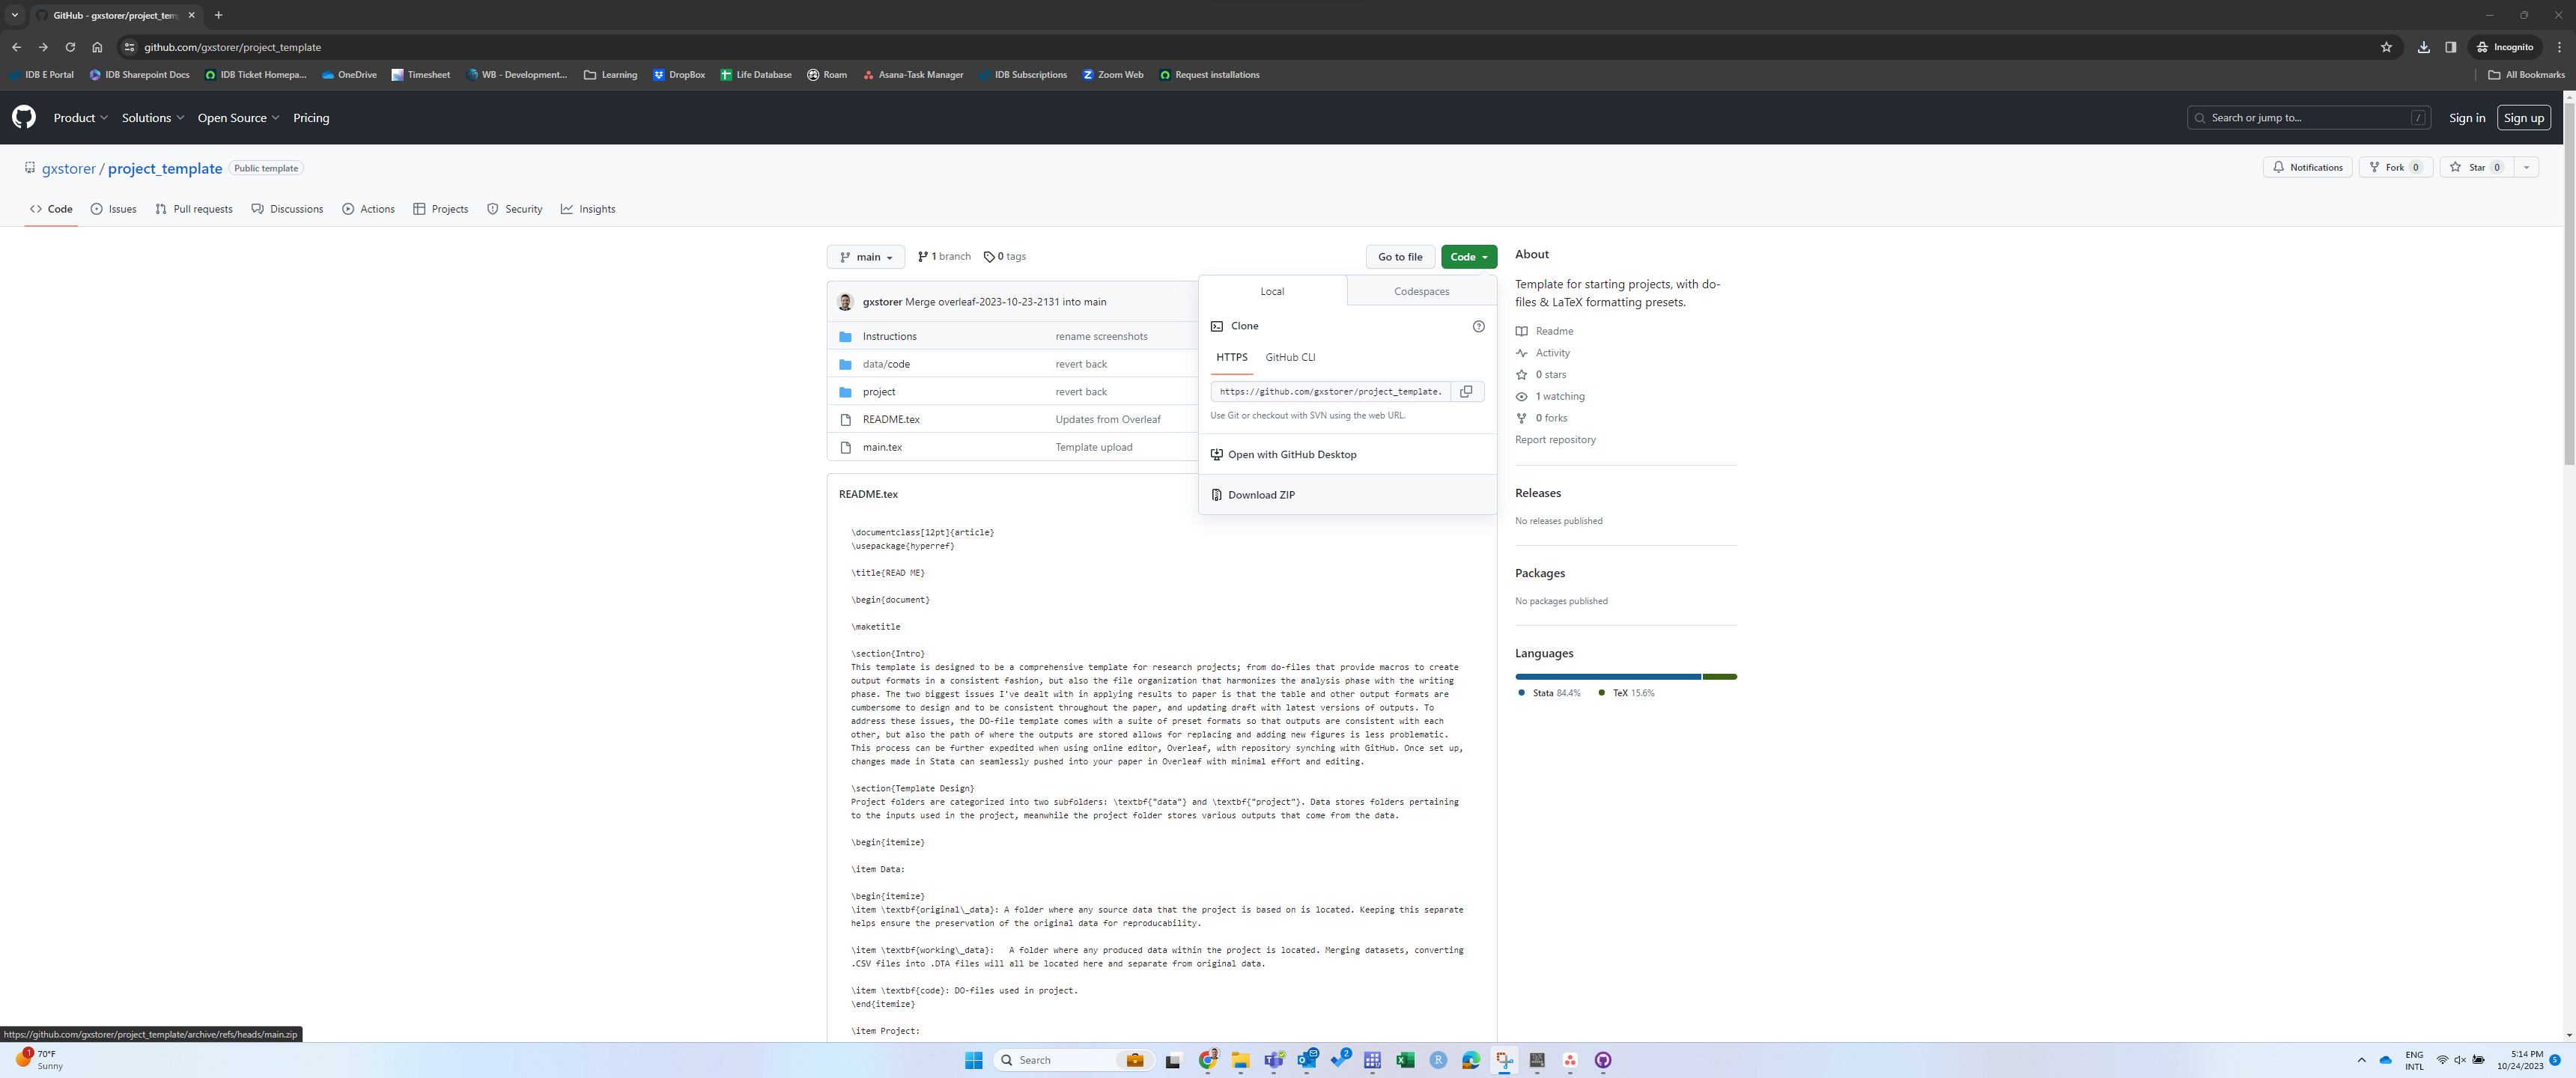
\includegraphics[width=1\linewidth]{Instructions/project_template_screenshots/project_template_001.png} \\

\section{Starting Overleaf Project}

First start by creating a new blank project in Overleaf. 
You could also use the import from GitHub or upload a .zip compressed file of the template folder, but I'll demonstrate with the blank project to be more straightforward. \\


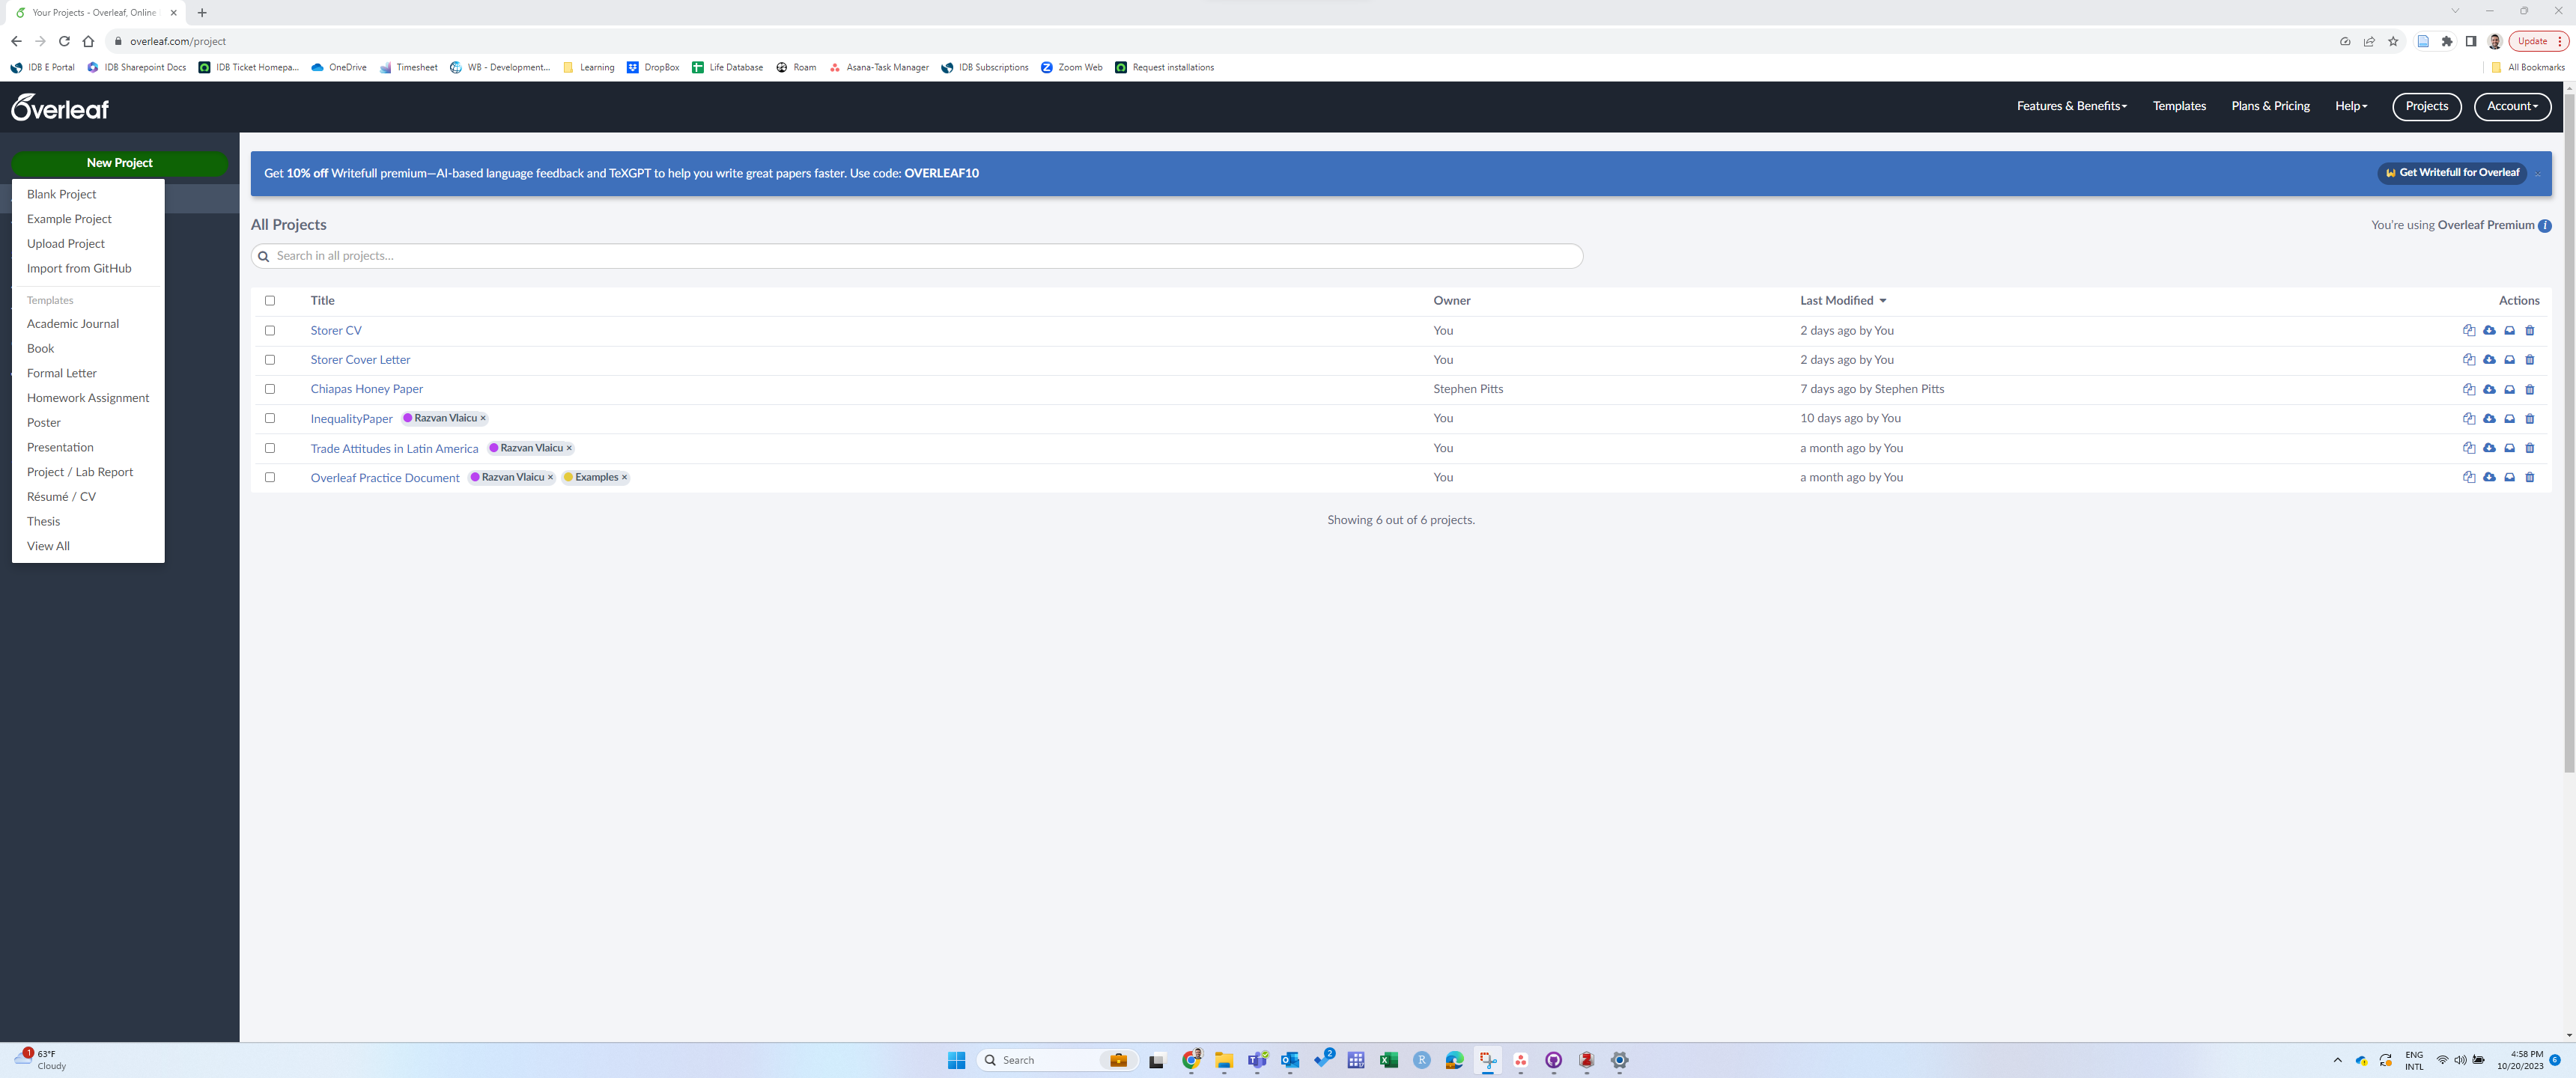
\includegraphics[width=1\textwidth]{Instructions/project_template_screenshots/project_template_01.png} \\

Once you've started a new project, click on the menu tab at the topleft corner of Overleaf, and select \textbf{GitHub}. \\

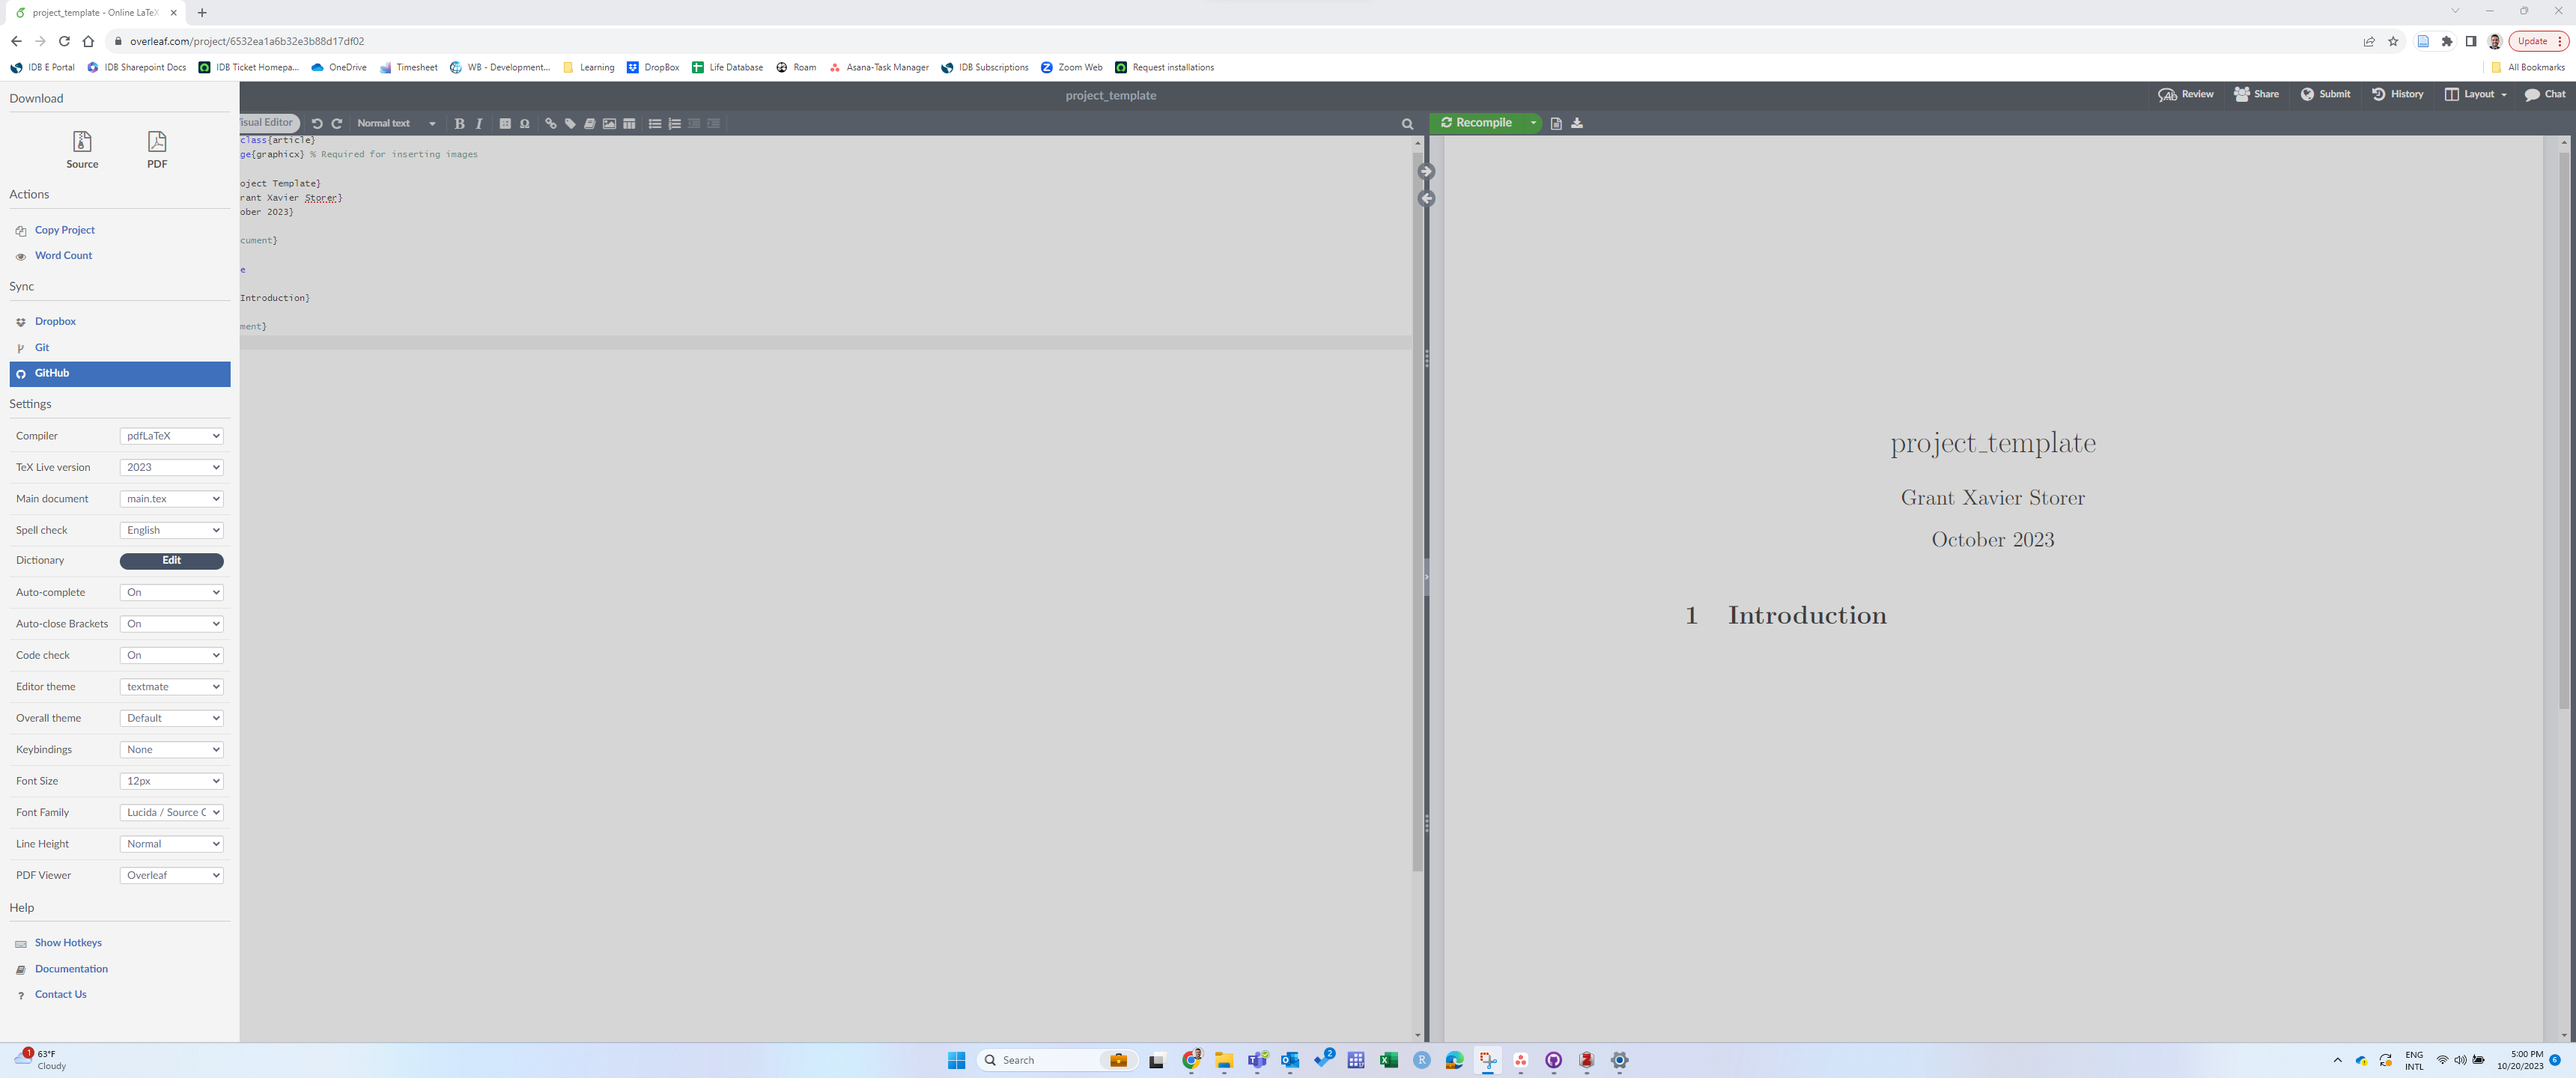
\includegraphics[width=1\textwidth]{Instructions/project_template_screenshots/project_template_02.png} \\

When you first start a project and select GitHub, it will display the menu to export project to GitHub. This will create a new repository on GitHub that is connected to this project on Overleaf. You can use any name you like for the project name, just know that this will be folder name in both GitHub and your local storage. \\

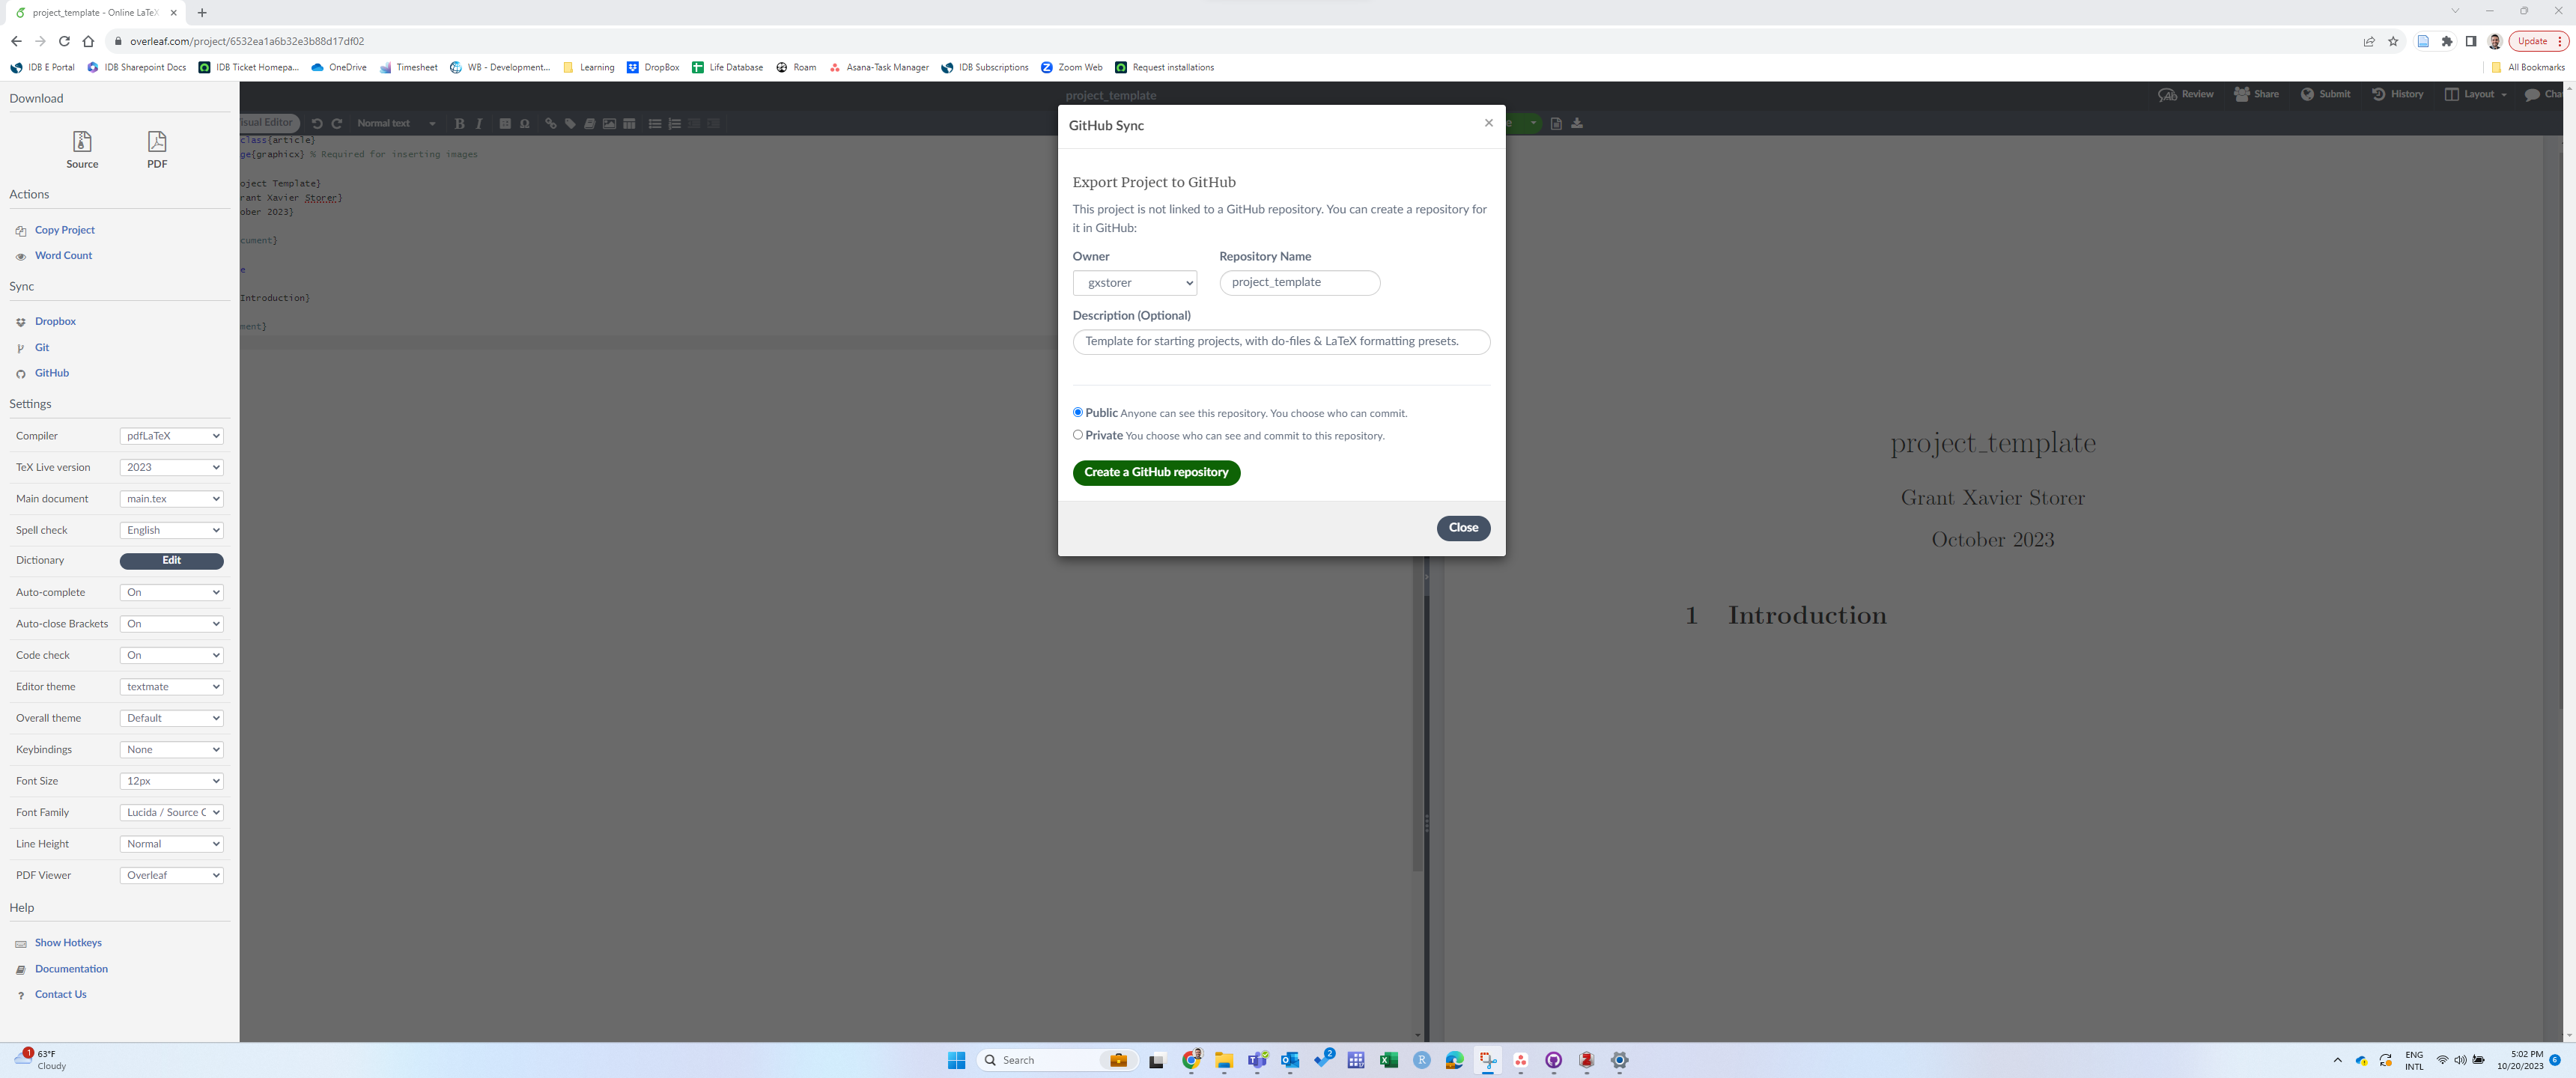
\includegraphics[width=1\textwidth]{Instructions/project_template_screenshots/project_template_03.png}\\


\section{GitHub Remote Repository}

Once you've created a repository through Overleaf, open/download \href{https://desktop.github.com/}{\underline{GitHub Desktop}}. Click on the \textbf{file} tab, and select \textbf{Clone a repository}. A pop-up window will show all repositories in your GitHub account, and select the name of the repository you created in Overleaf. GitHub will default to storing these files in its own folder that is saved on your local drive, but you can manually change the path of where these files are stored. \\

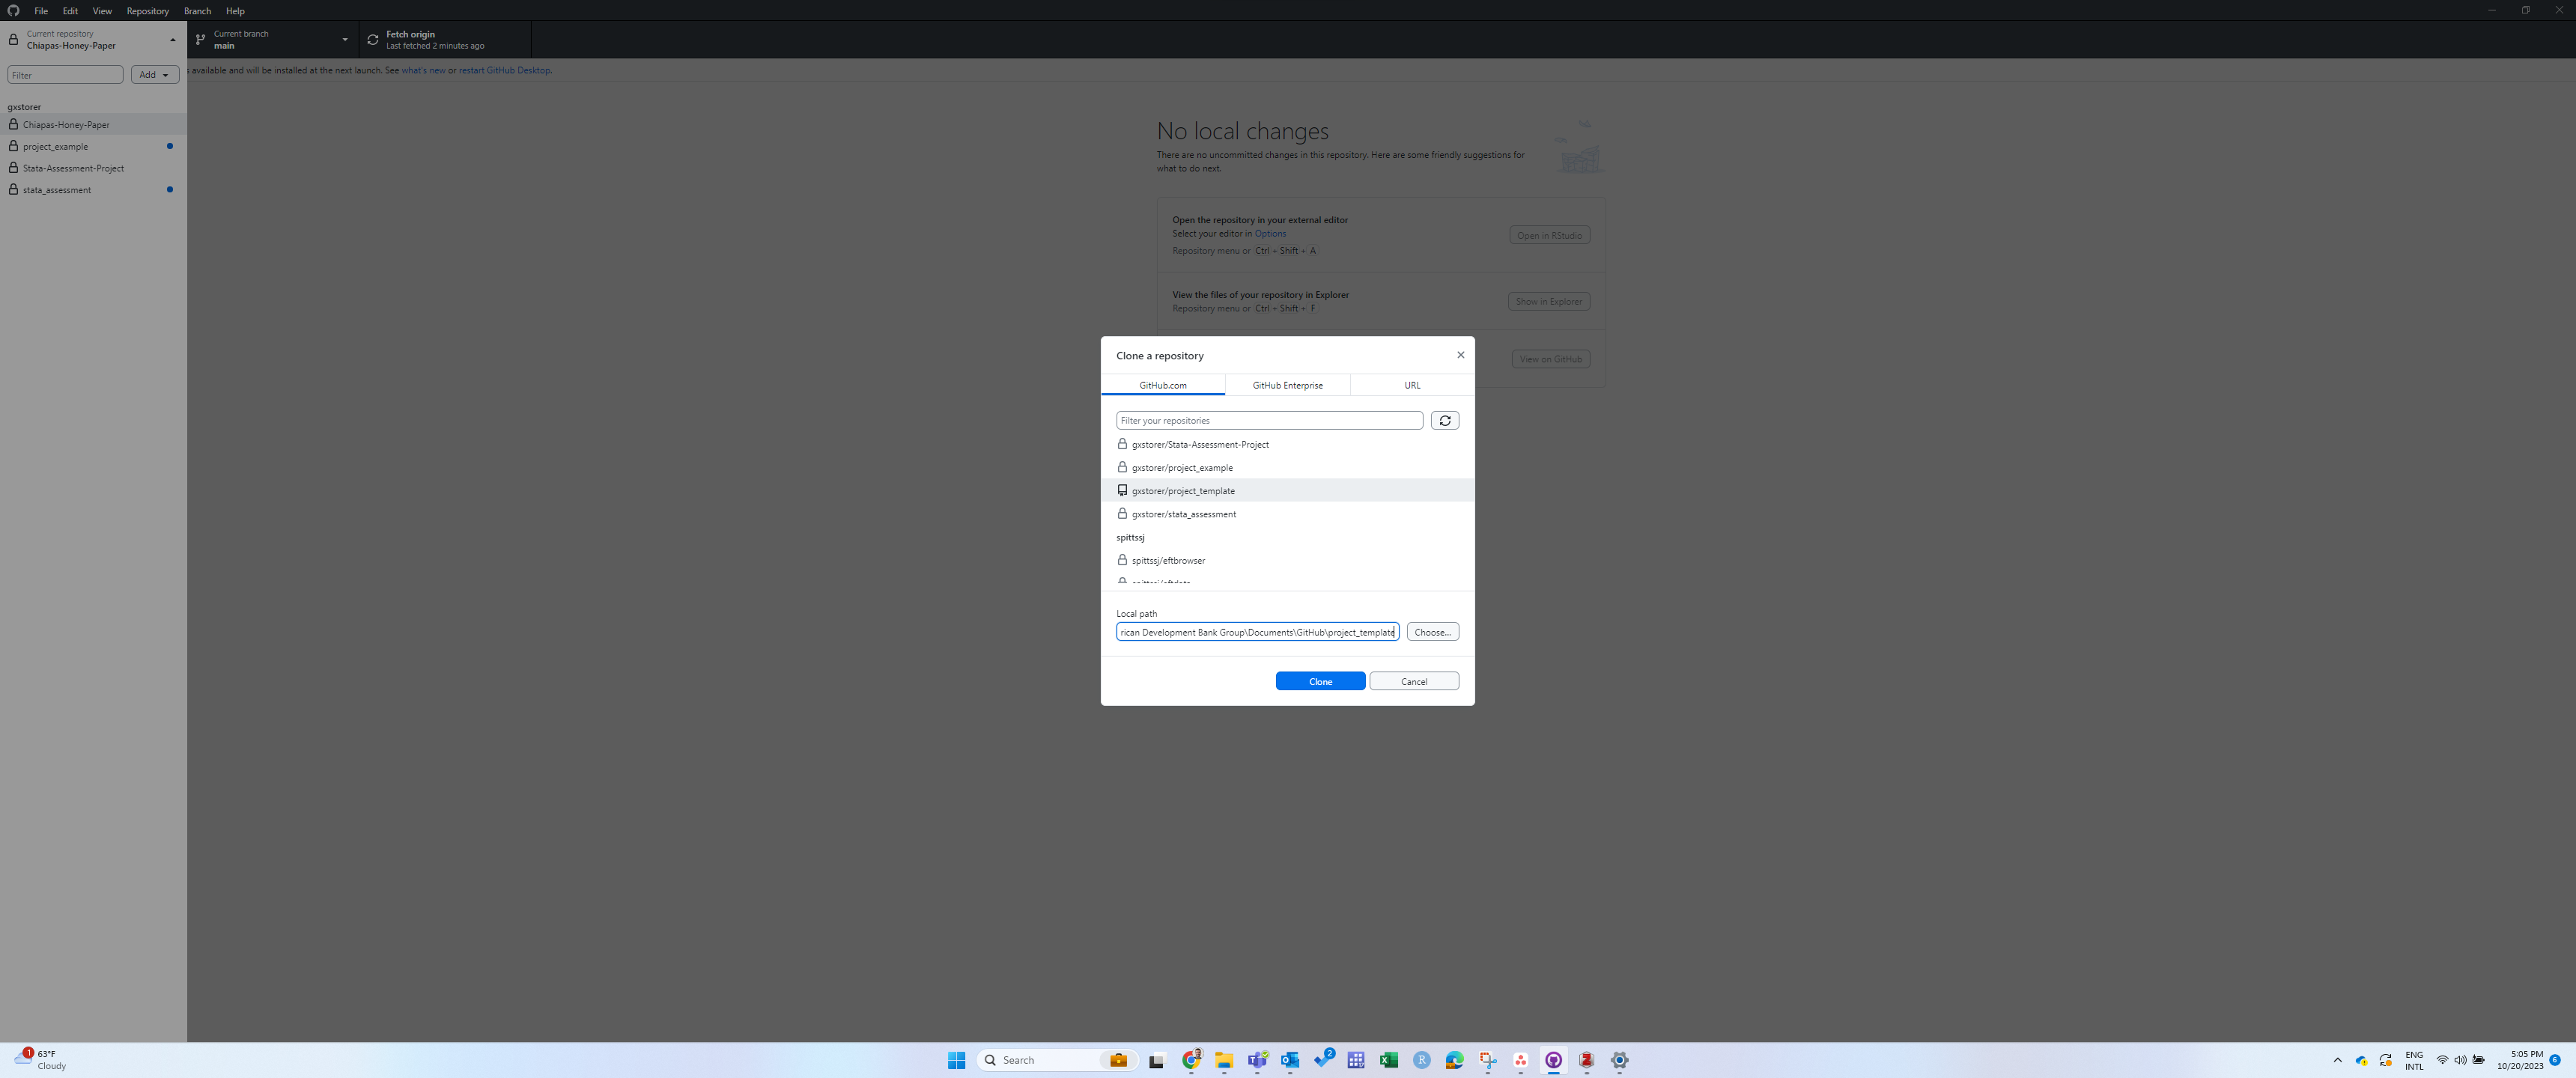
\includegraphics[width=1\textwidth]{Instructions/project_template_screenshots/project_template_04.png} \\

Once you've successfully cloned your repository, you should be able to find the default \textbf{main.tex} file that Overleaf creates at the beginning of the new project. \\

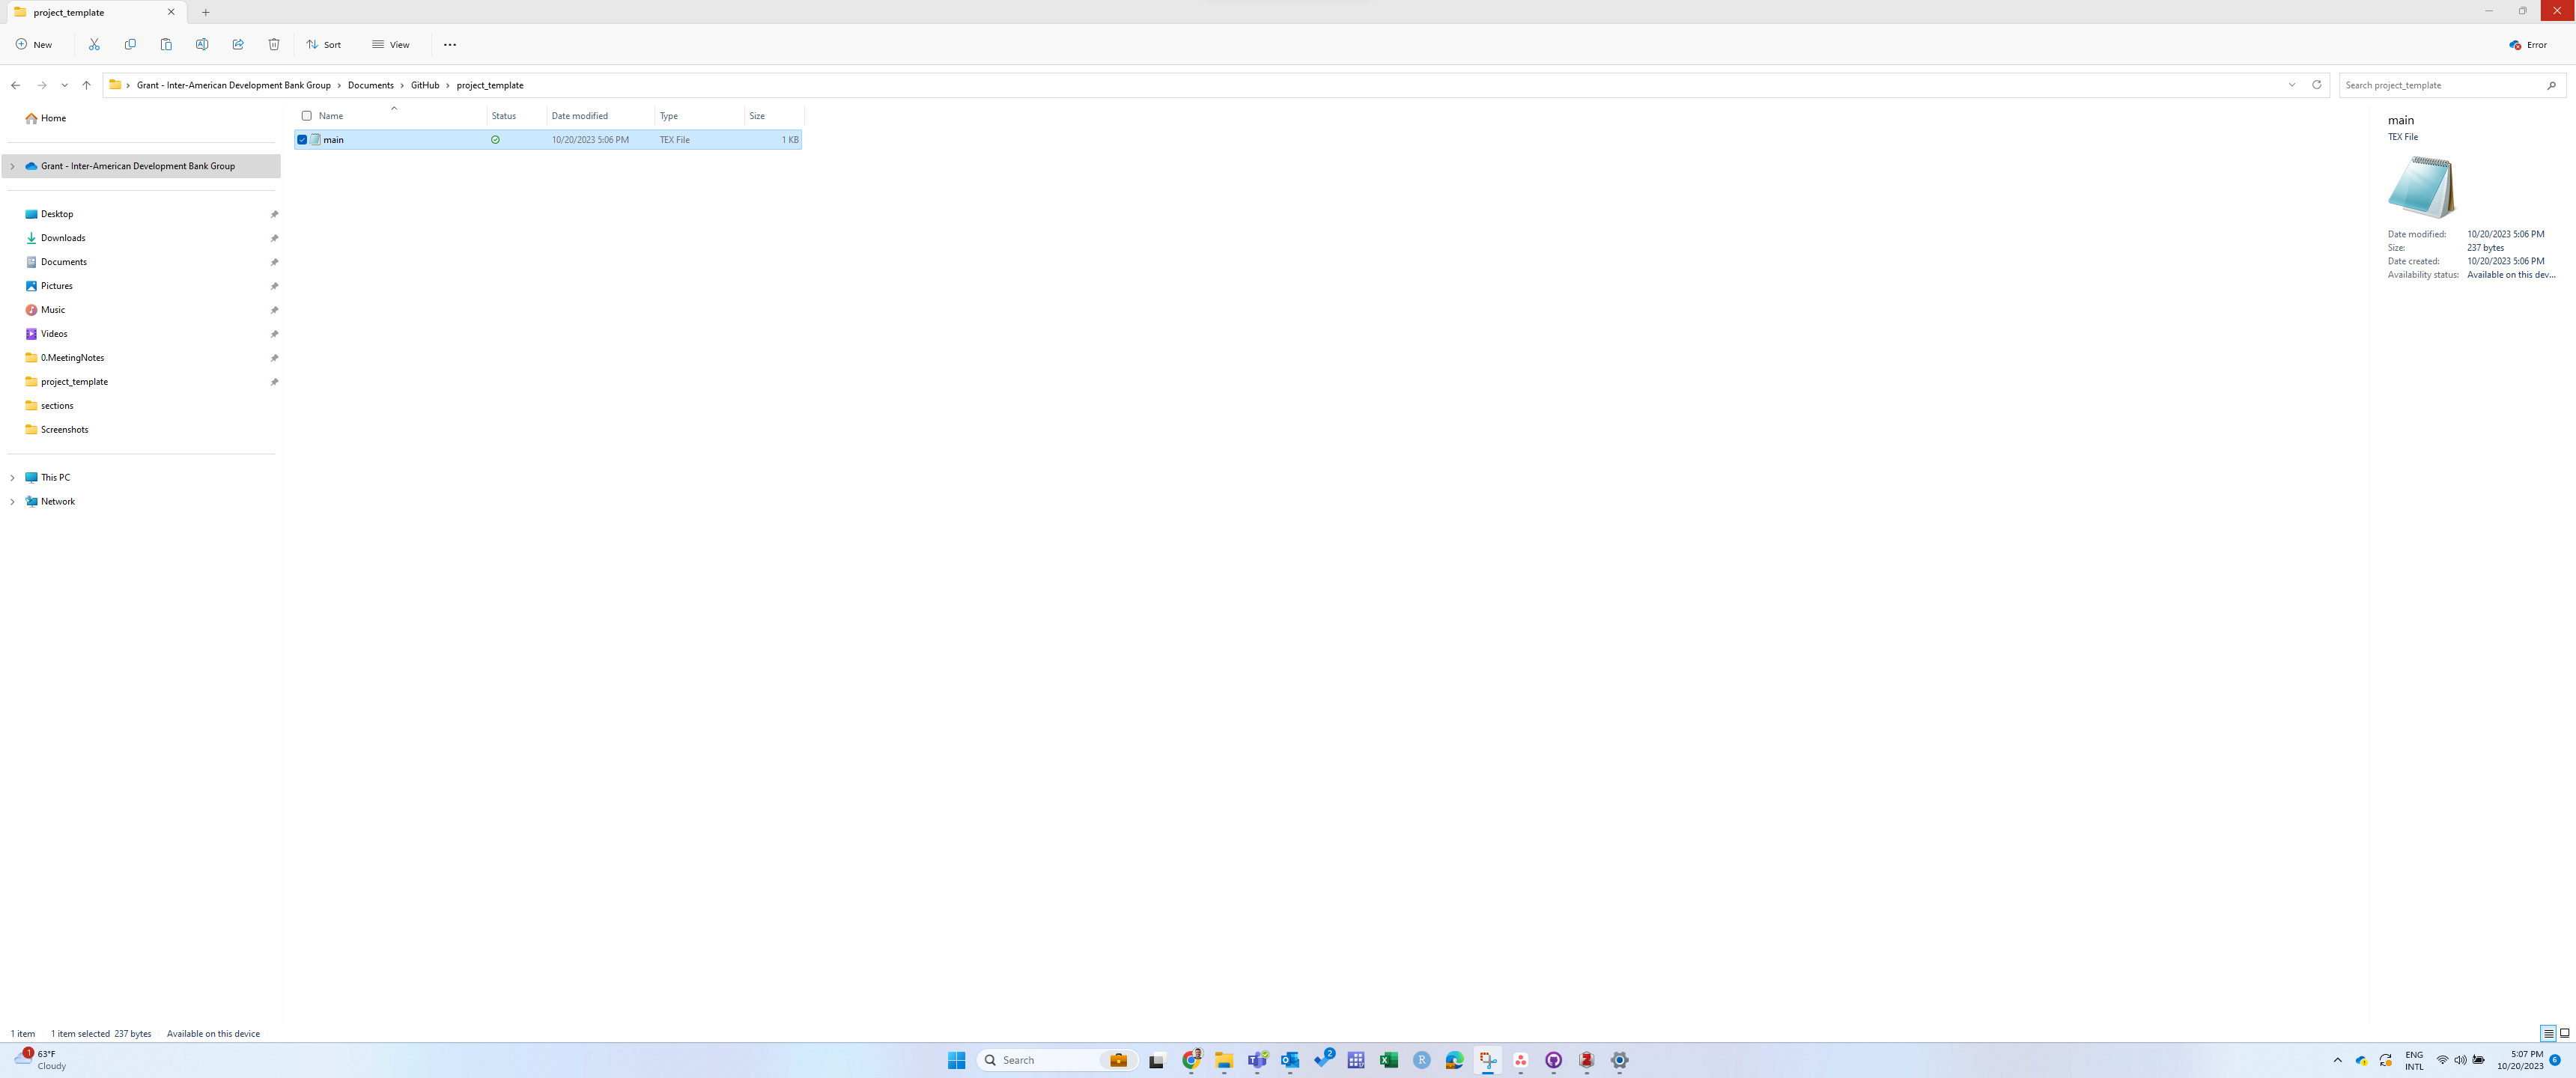
\includegraphics[width=1\textwidth]{Instructions/project_template_screenshots/project_template_05.png} \\

Next step is to replace this file with the \textbf{project\_template} files. You will no longer need the file created by Overleaf, and if you keep the files names from the template, you can either overwrite the Overleaf main.tex, or just delete it and replace with the template main.tex. \\

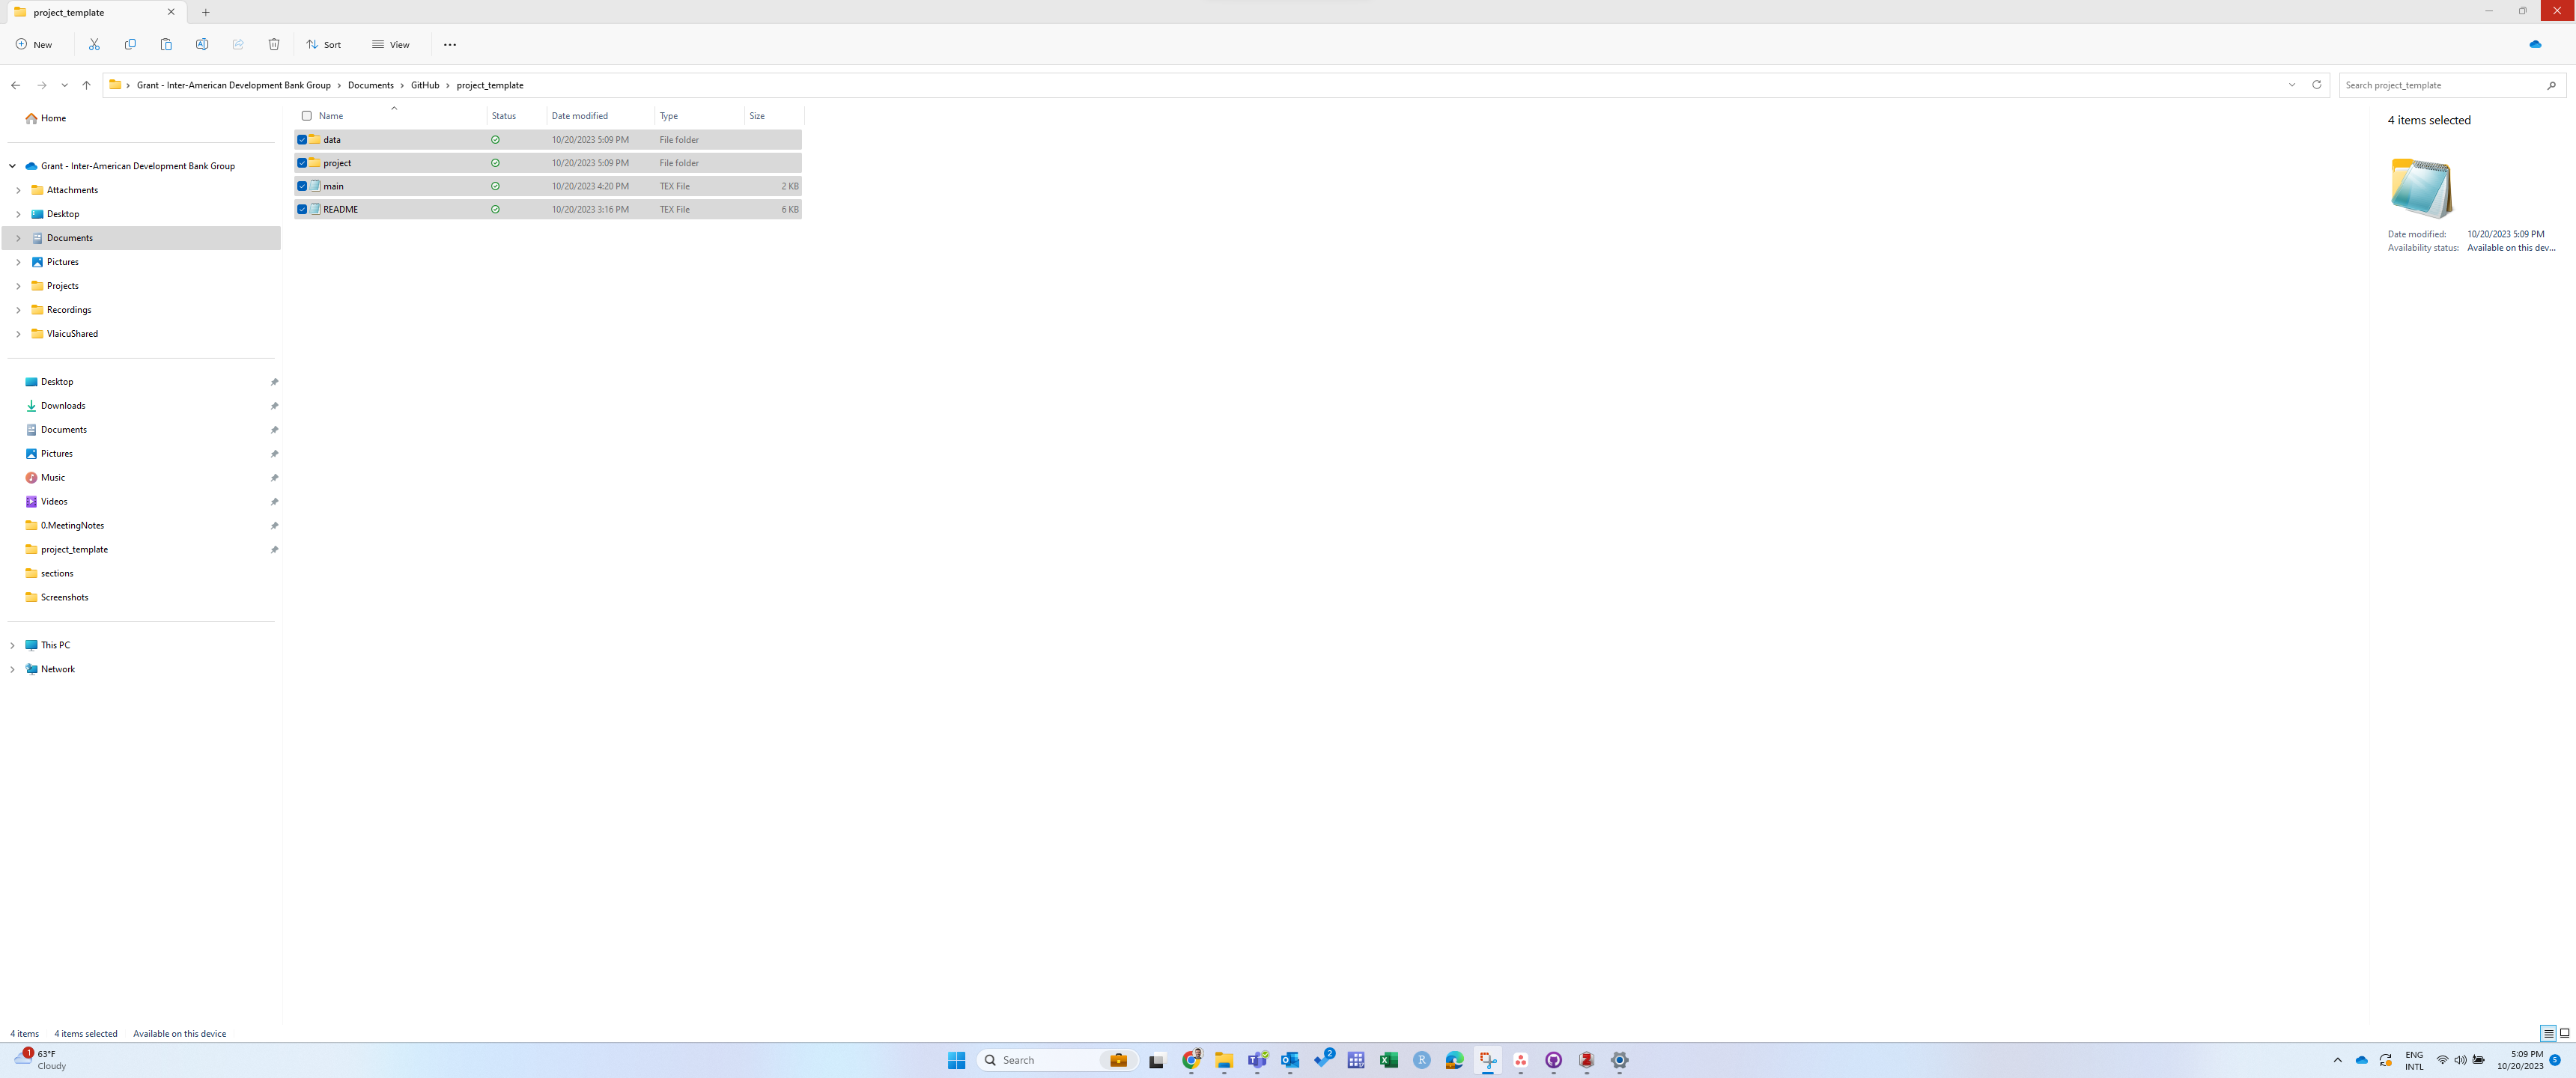
\includegraphics[width=1\textwidth]{Instructions/project_template_screenshots/project_template_06.png} \\

\section{Updating Overleaf}

Once you've moved the template files into your local folder, go back to GitHub Desktop, and push changes to main. GitHub Desktop will show all the changes you made locally that are not online yet, and using the window in the bottom-left corner, \textbf{Commit to main} all these changes.  \\

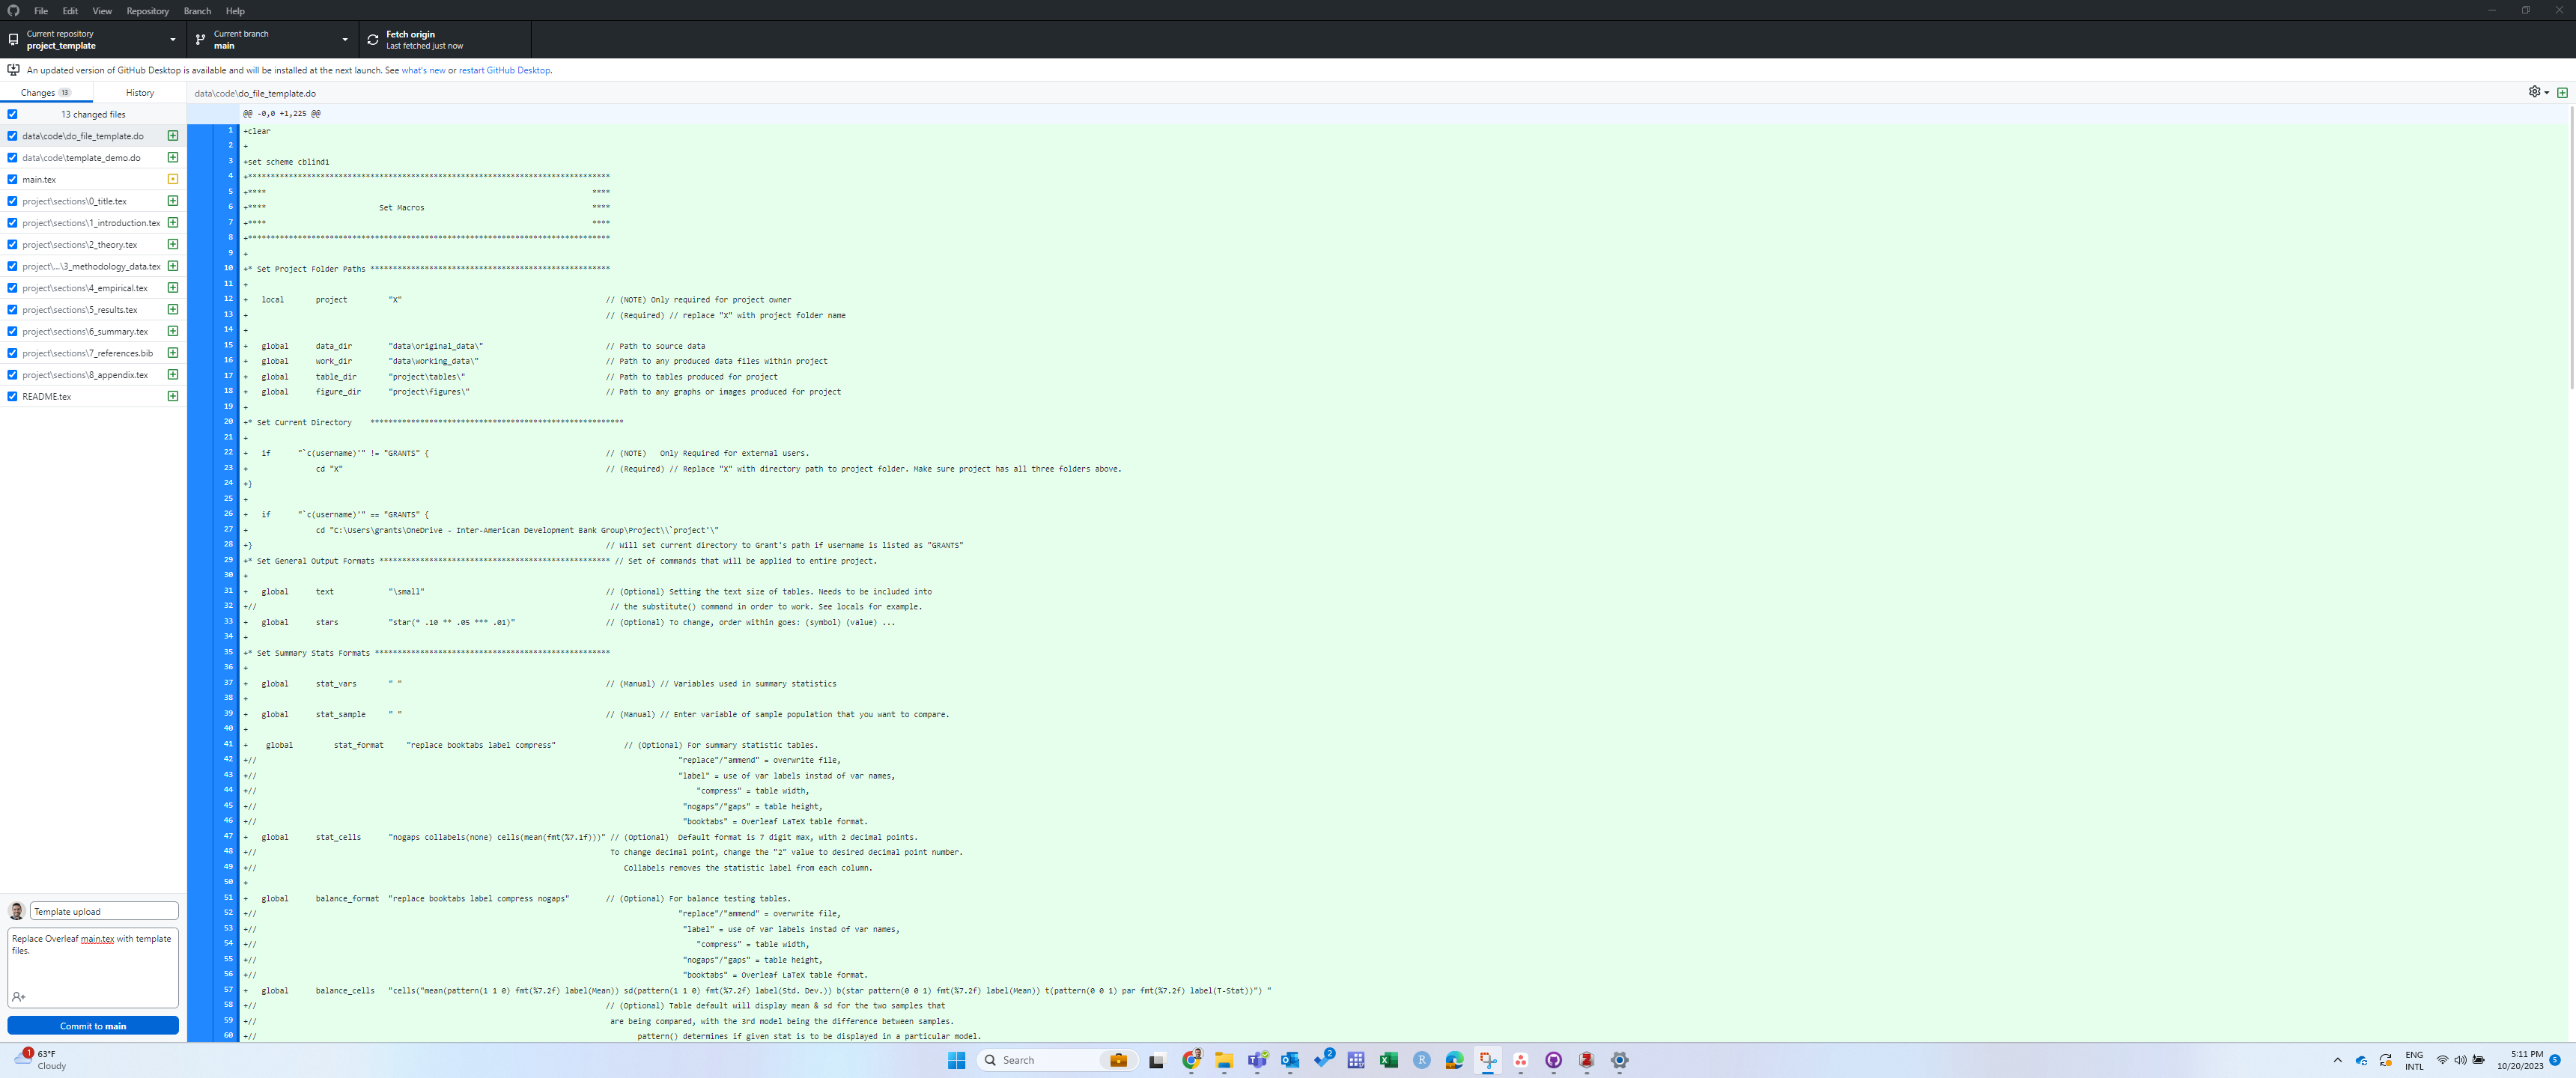
\includegraphics[width=1\textwidth]{Instructions/project_template_screenshots/project_template_07.png} \\

This just saves the changes, but have not yet shown up online. Click on the push origin button to push all commits to the online repository. \\

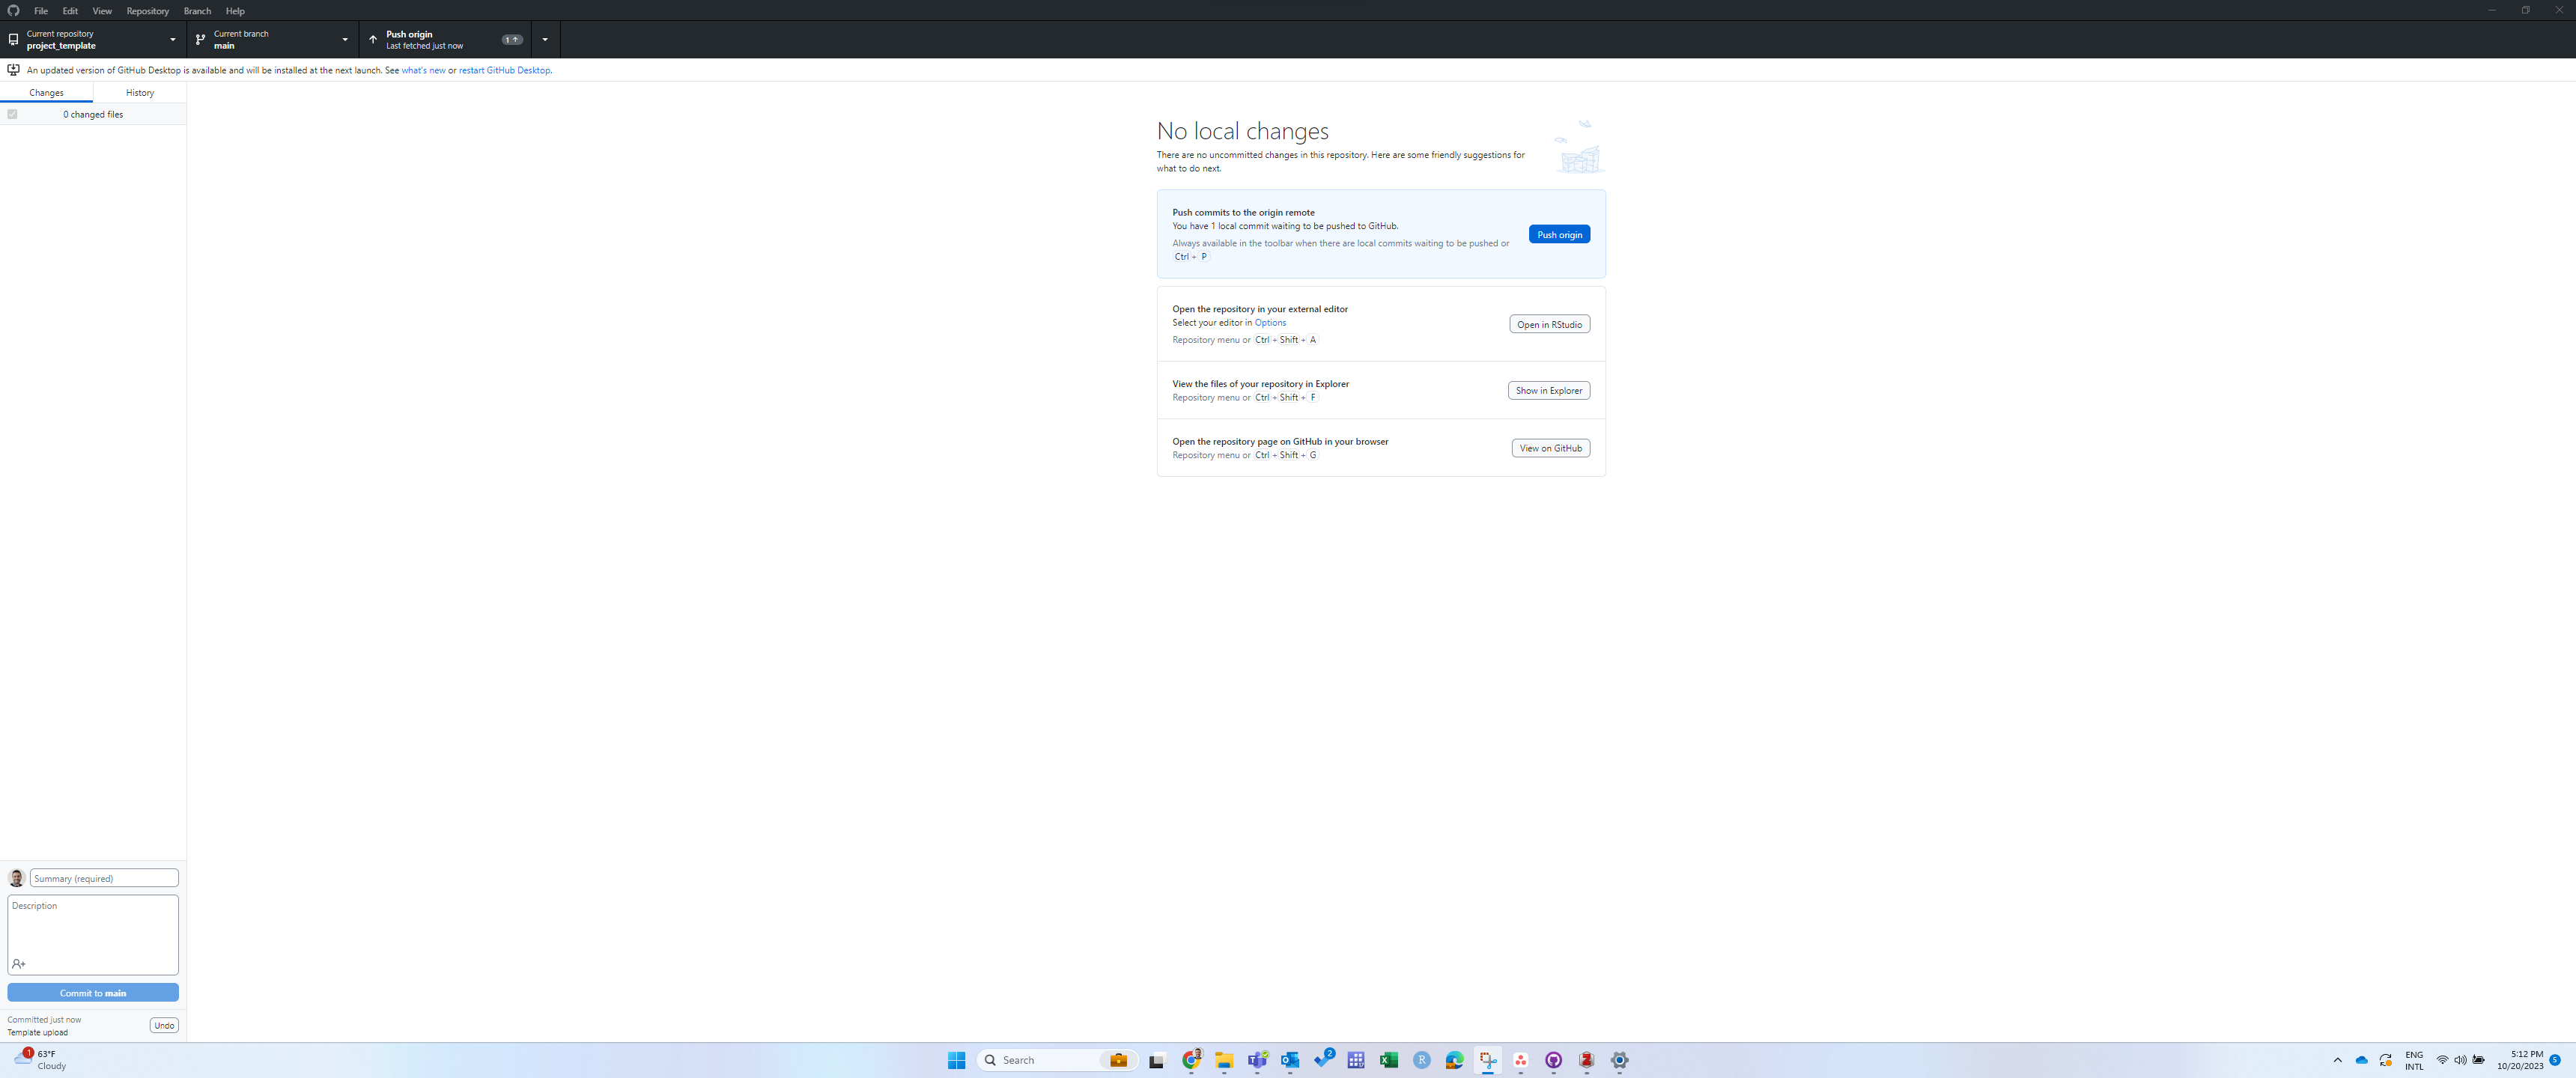
\includegraphics[width=1\textwidth]{Instructions/project_template_screenshots/project_template_08.png} \\

Now return to the Overleaf project, and select the GitHub tab from the menu again. You'll see that there's now a push/pull options related to the remote repository. Additionally, since you pushed an update to your GitHub account, you'll see that Overleaf automatically identified this change and includes the comments you entered with that commit. Click on the \textbf{Pull GitHub changs into Overleaf} button. \\

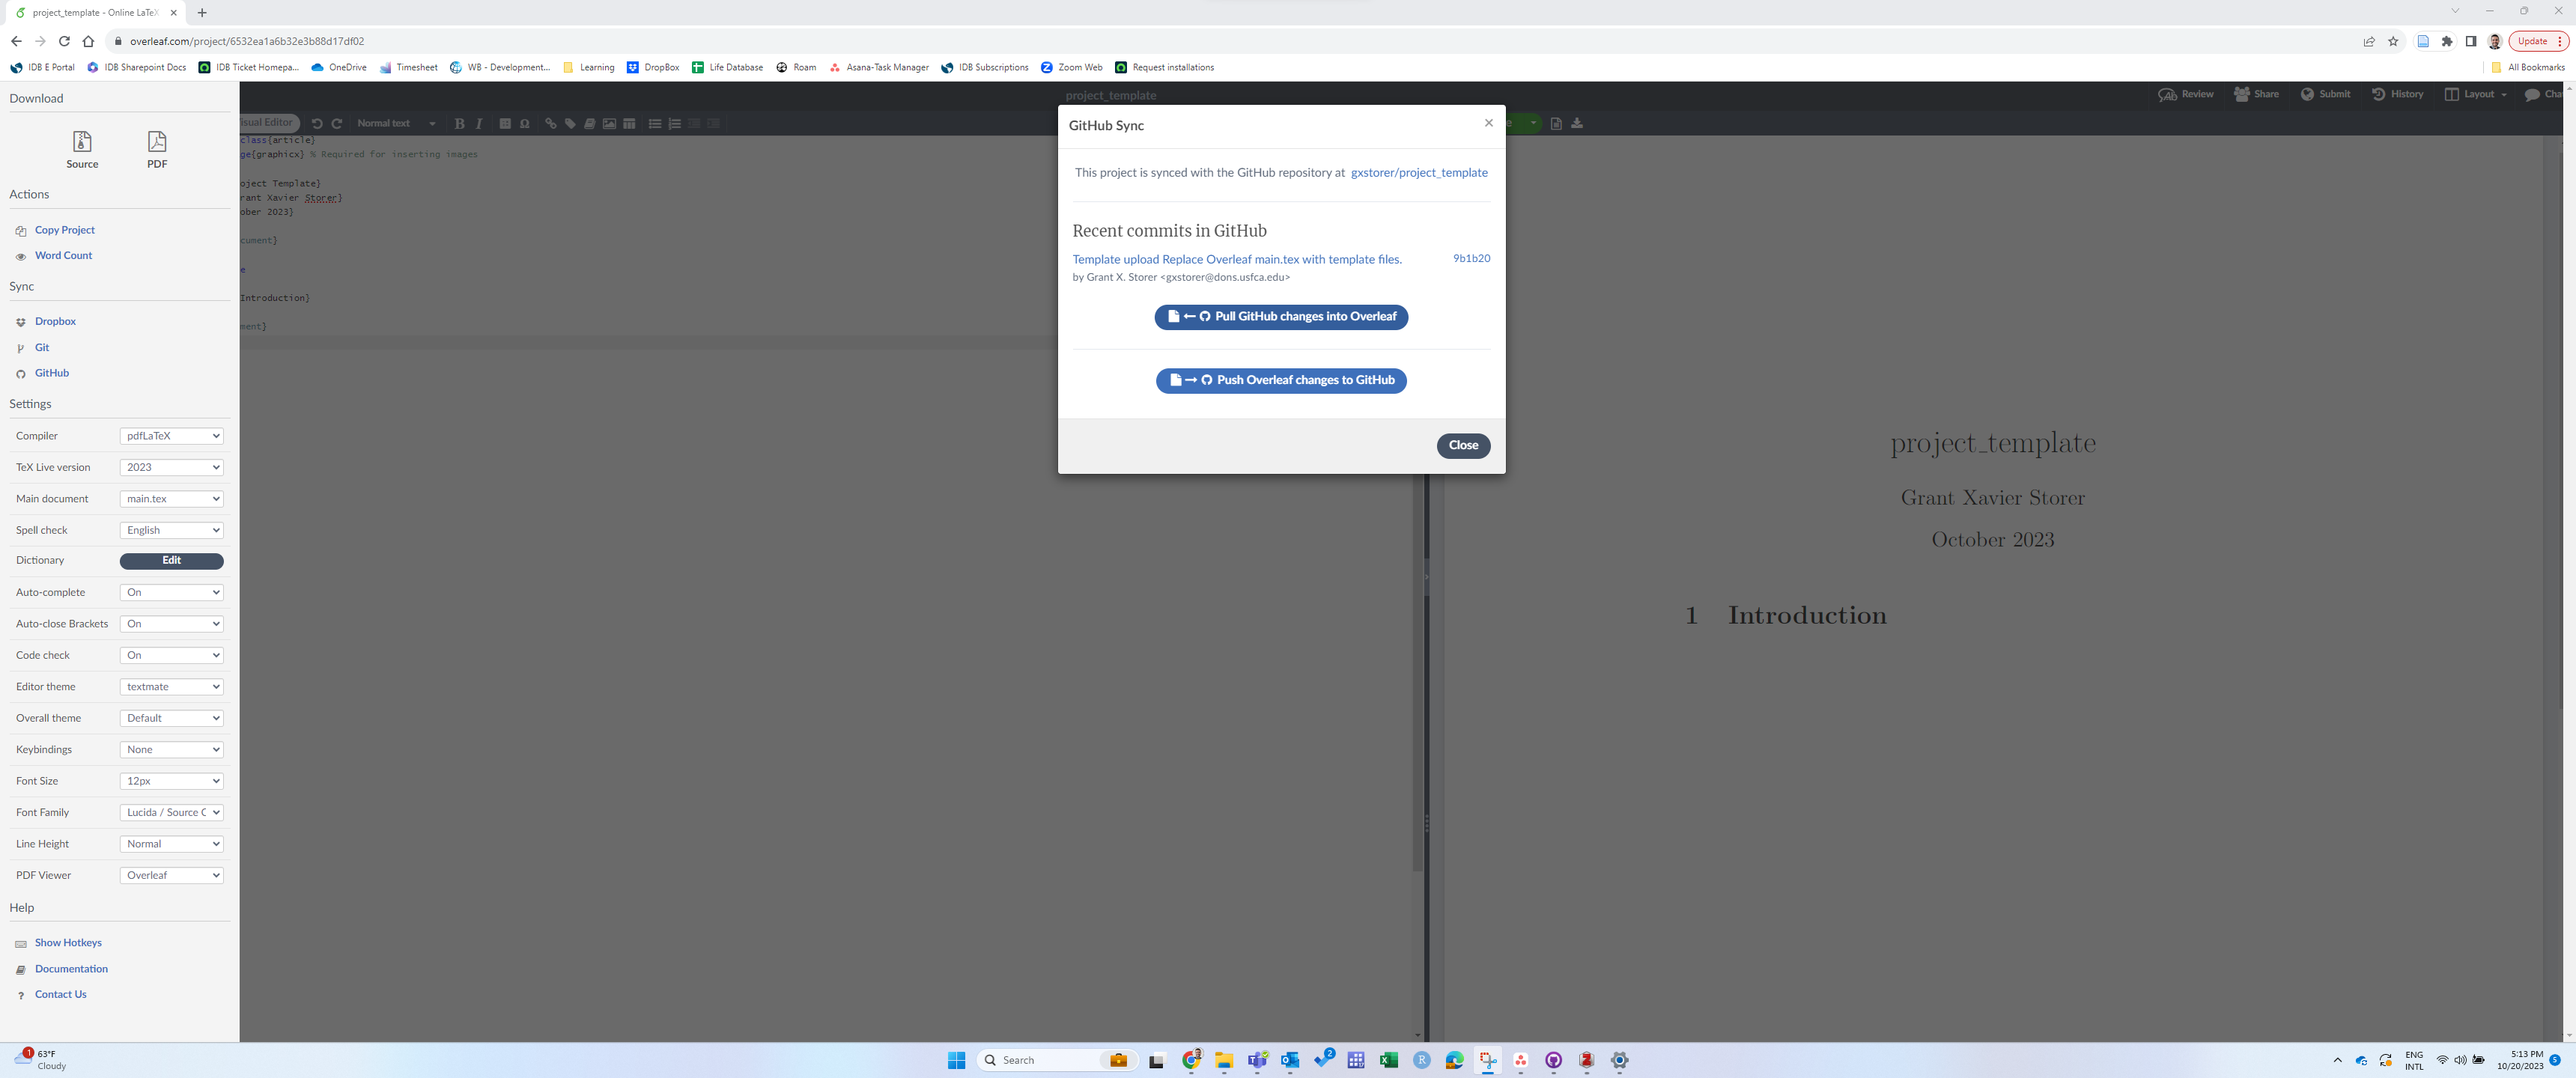
\includegraphics[width=1\textwidth]{Instructions/project_template_screenshots/project_template_09.png} \\

Once the changes have been pulled, you'll see that your Overleaf project now has all the files from the project\_template folder and you'll be able to compile the template version of your document. \\

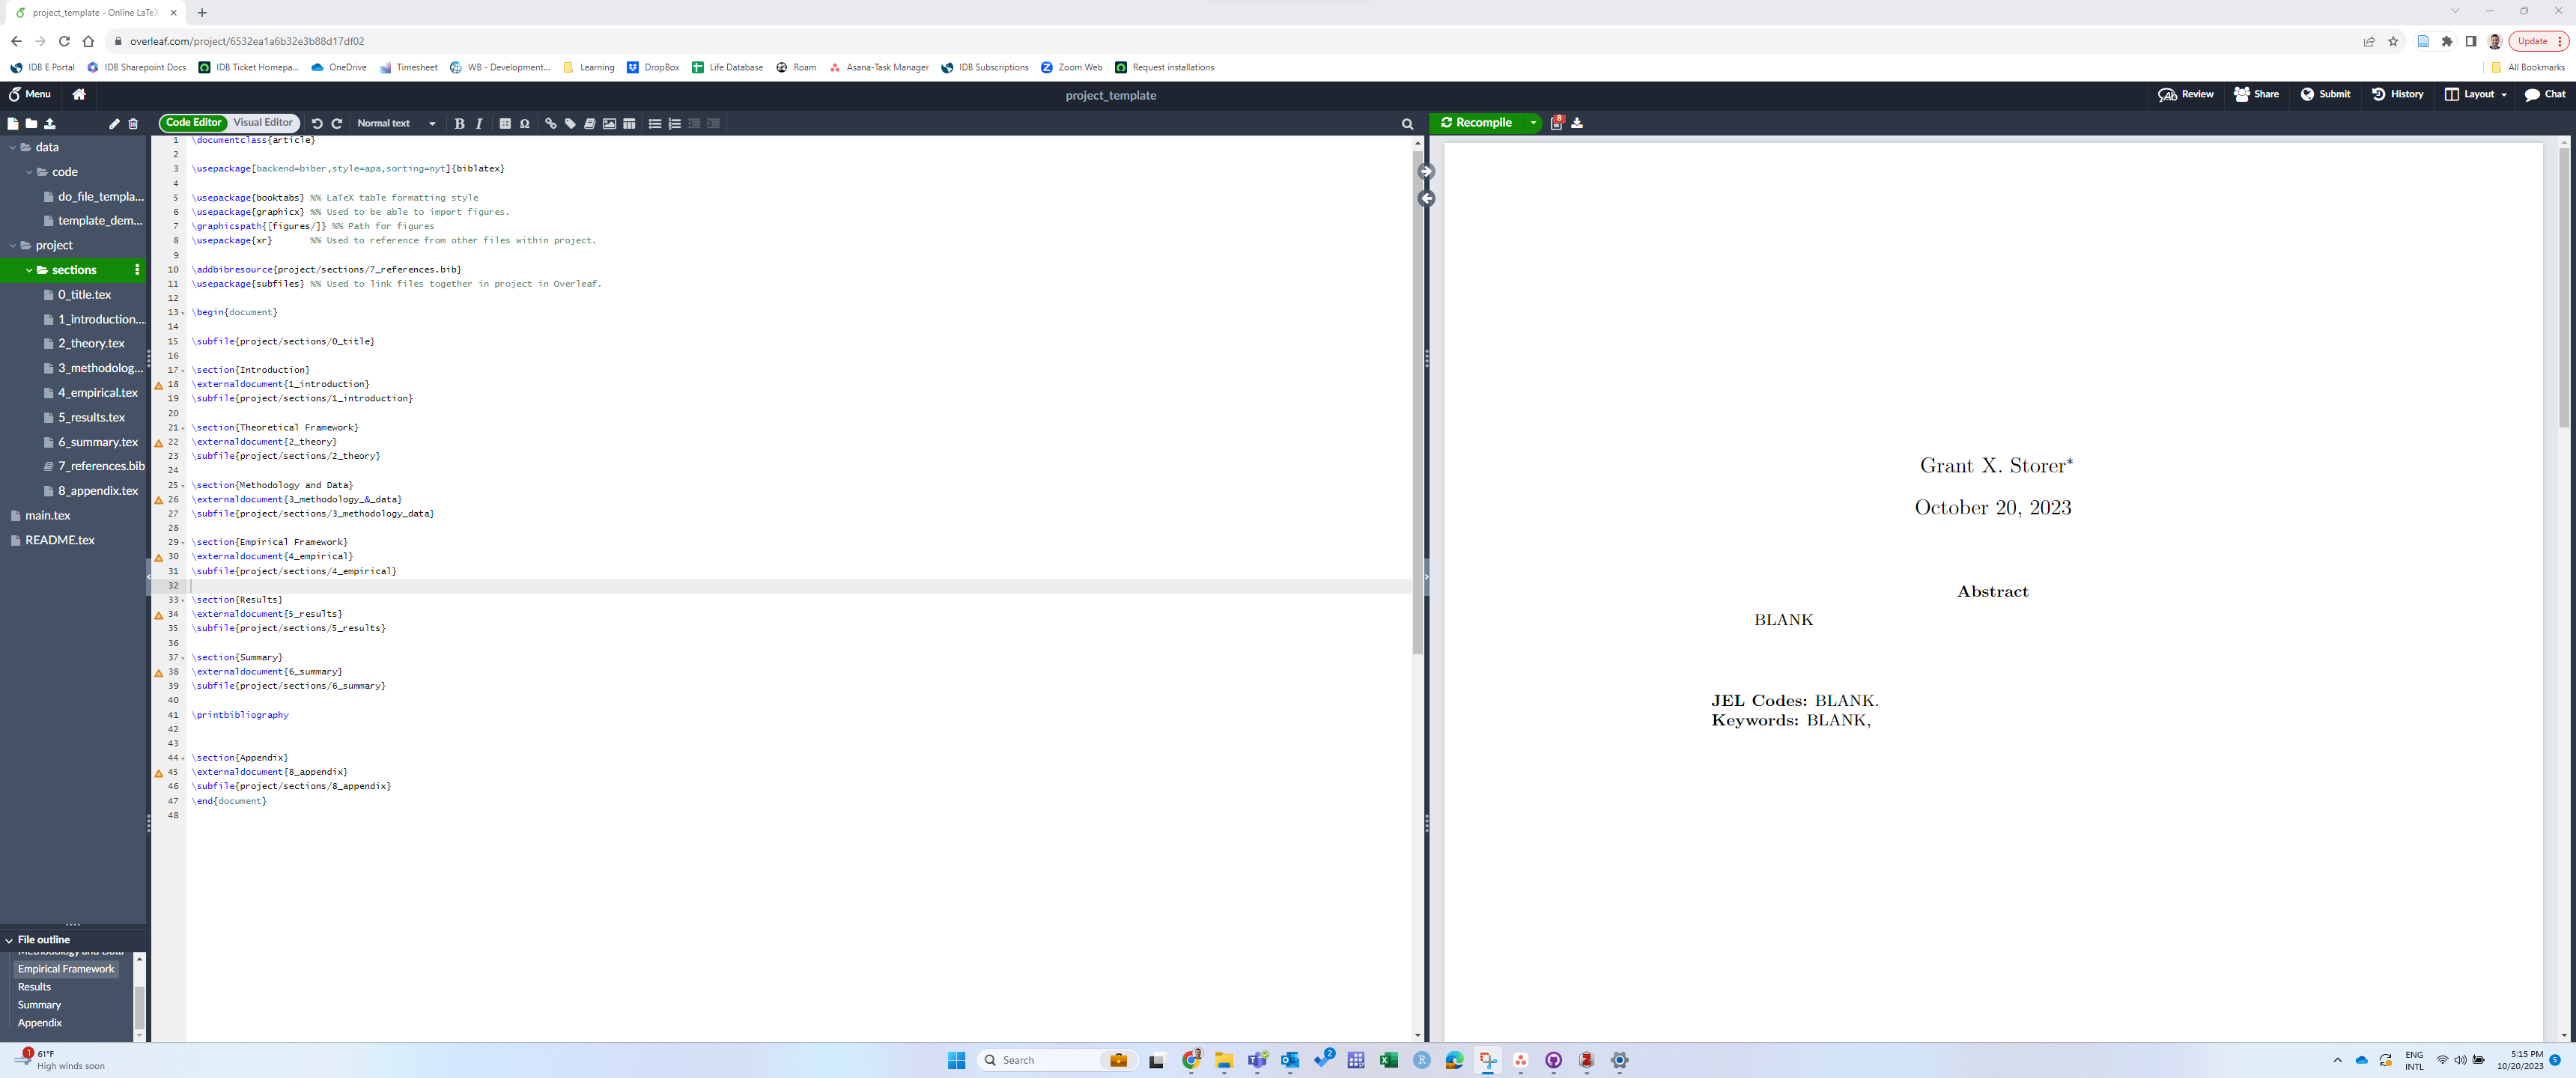
\includegraphics[width=1\textwidth]{Instructions/project_template_screenshots/project_template_10.png} \\

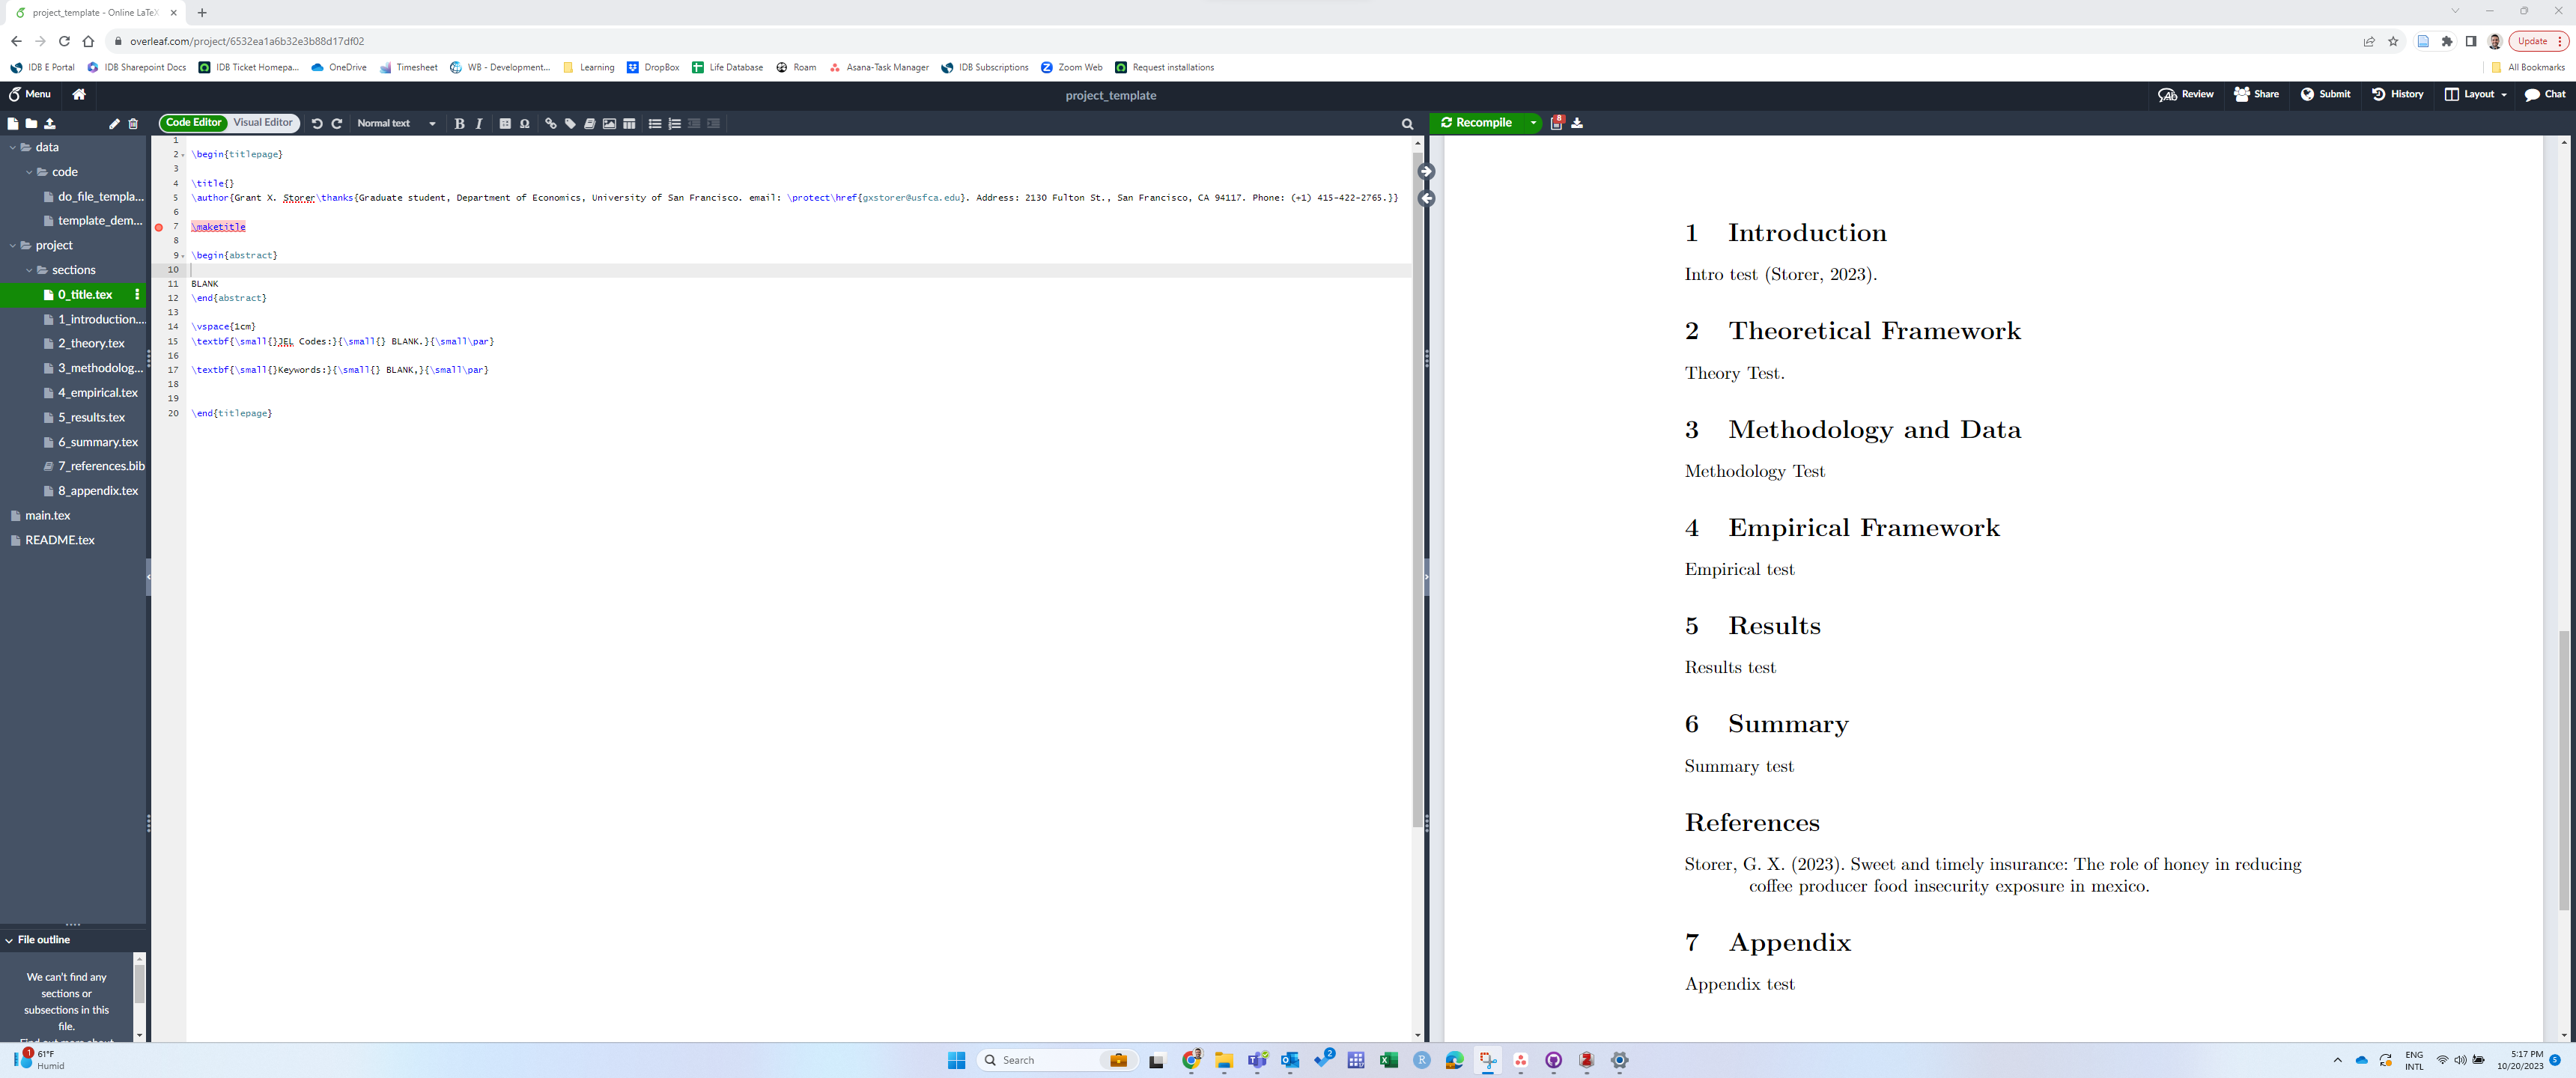
\includegraphics[width=1\textwidth]{Instructions/project_template_screenshots/project_template_11.png} \\

\section{Using Do-file}

Once this link has been set, this will now allow you to make changes on either the analysis side or the write-up, and it'll sync up on the other end. To demonstrate this process, we'll emulate the process of first producing figures and tables from the analysis side and moving that into the write-up. So return to the local site of your project, and go to the \textbf{data / code} folder and select the \textbf{template\_demo.dta} (or just open up Stata, and open this file with the \textbf{use} command).

This demo do-file can almost run right out of box, except to make sure you have the following packages installed in Stata: \textbf{ ESTOUT, REGHDFE \& SCHEMEPACK}, and to determine the path to the project within the do-file (line 24 in the script, or if you want to make this wholly your own: lines 23-28, and replace the username GRANTS with your Stata username). The README doc explains a bit more of how the do-file is constructed, but for now, you can just make these required changes and run the do-file, and it'll produce a few tables and graphs, which these outputs will automatically be saved in the \textbf{project / tables} or \textbf{project / figures} folders. \\

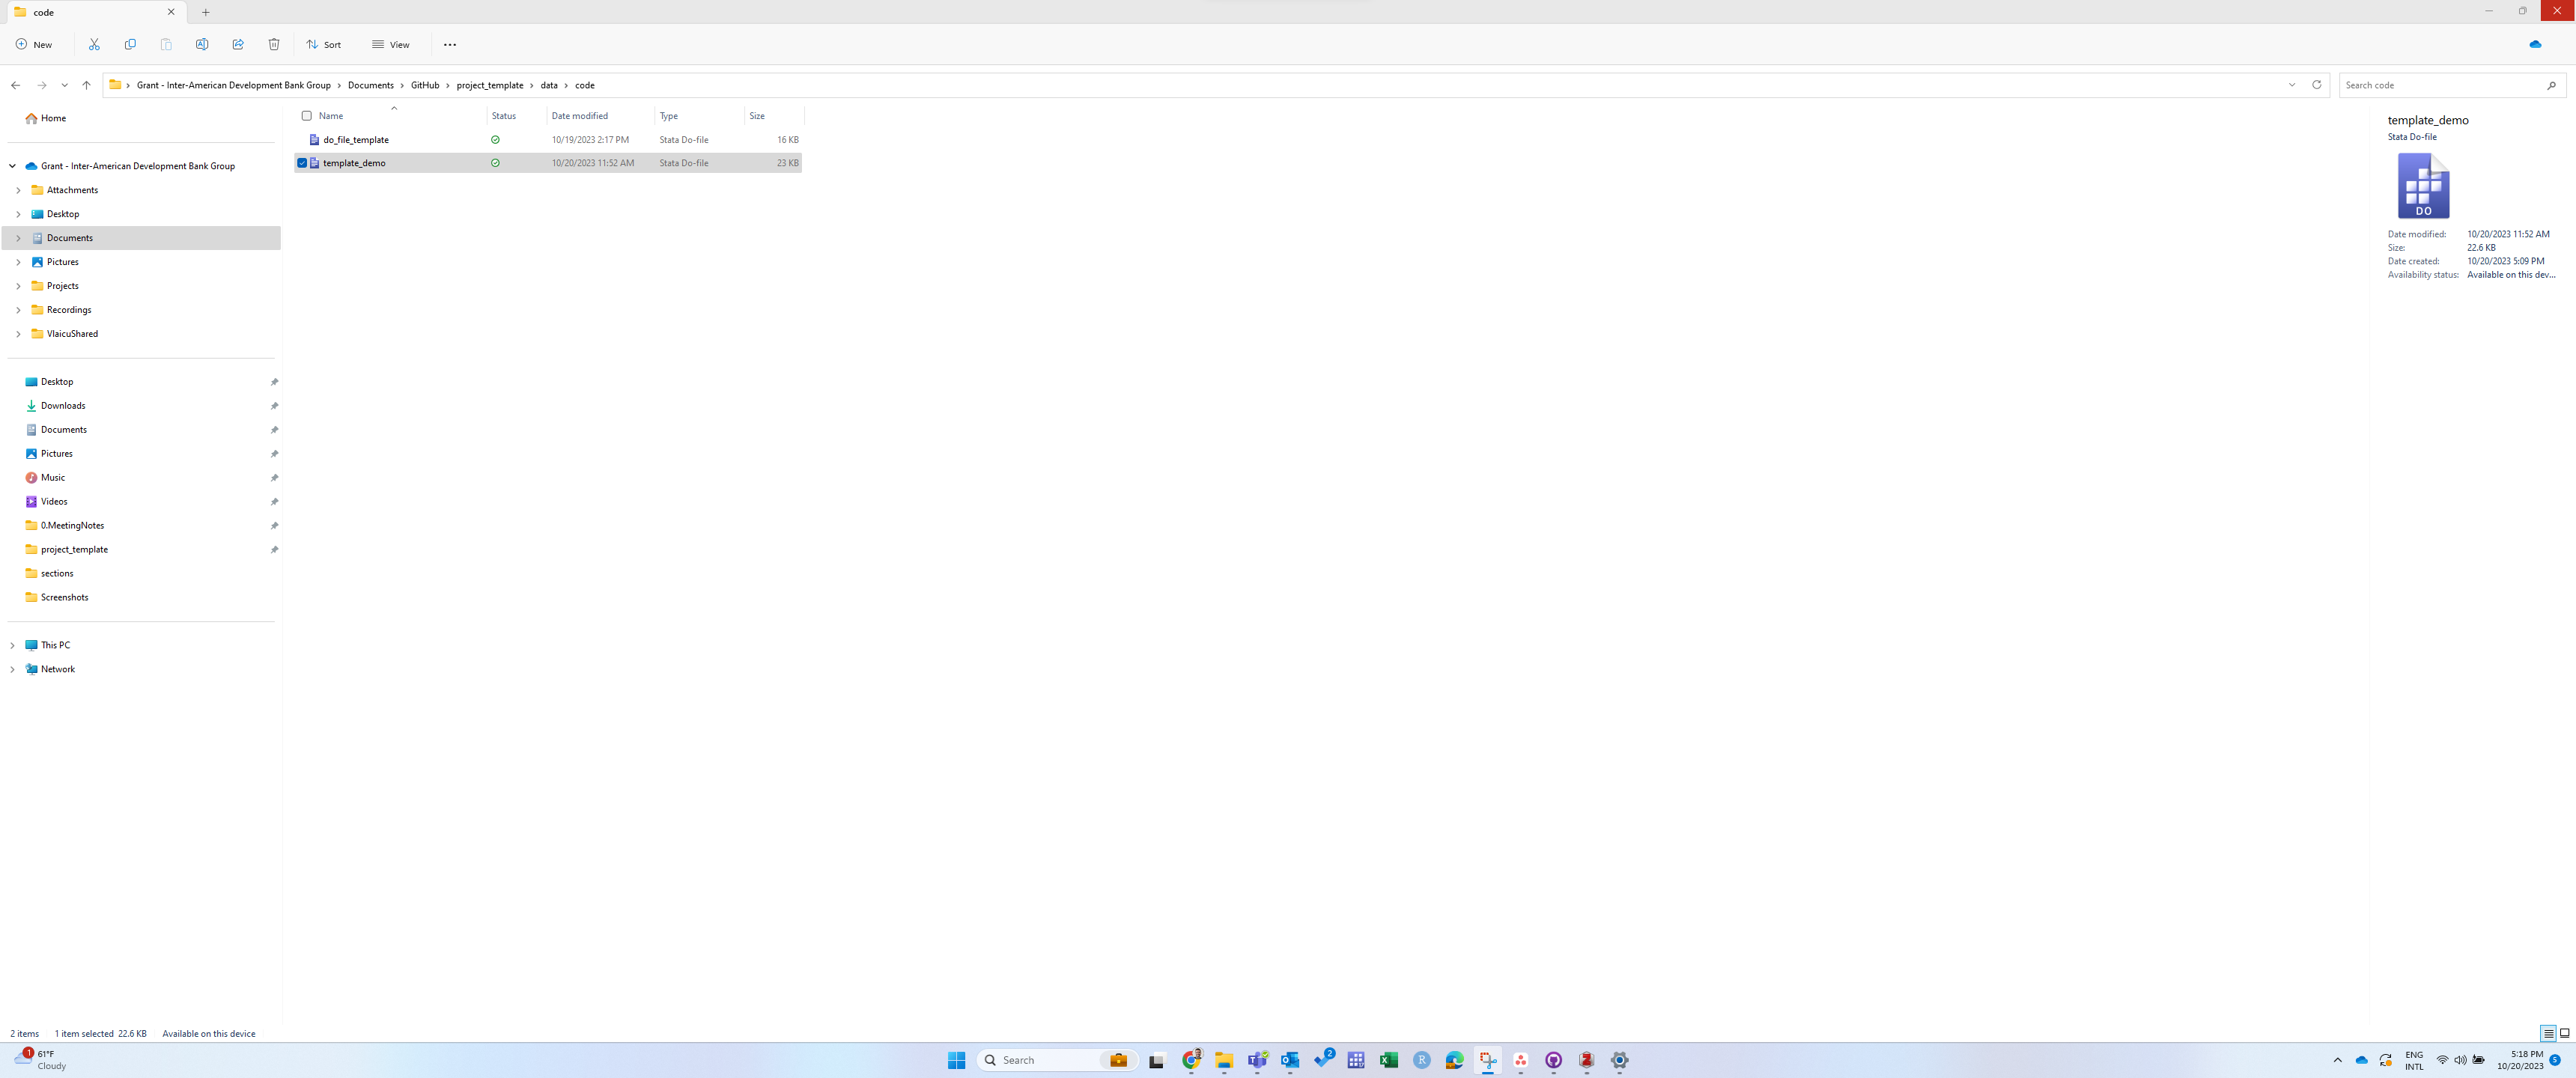
\includegraphics[width=1\textwidth]{Instructions/project_template_screenshots/project_template_13.png} \\

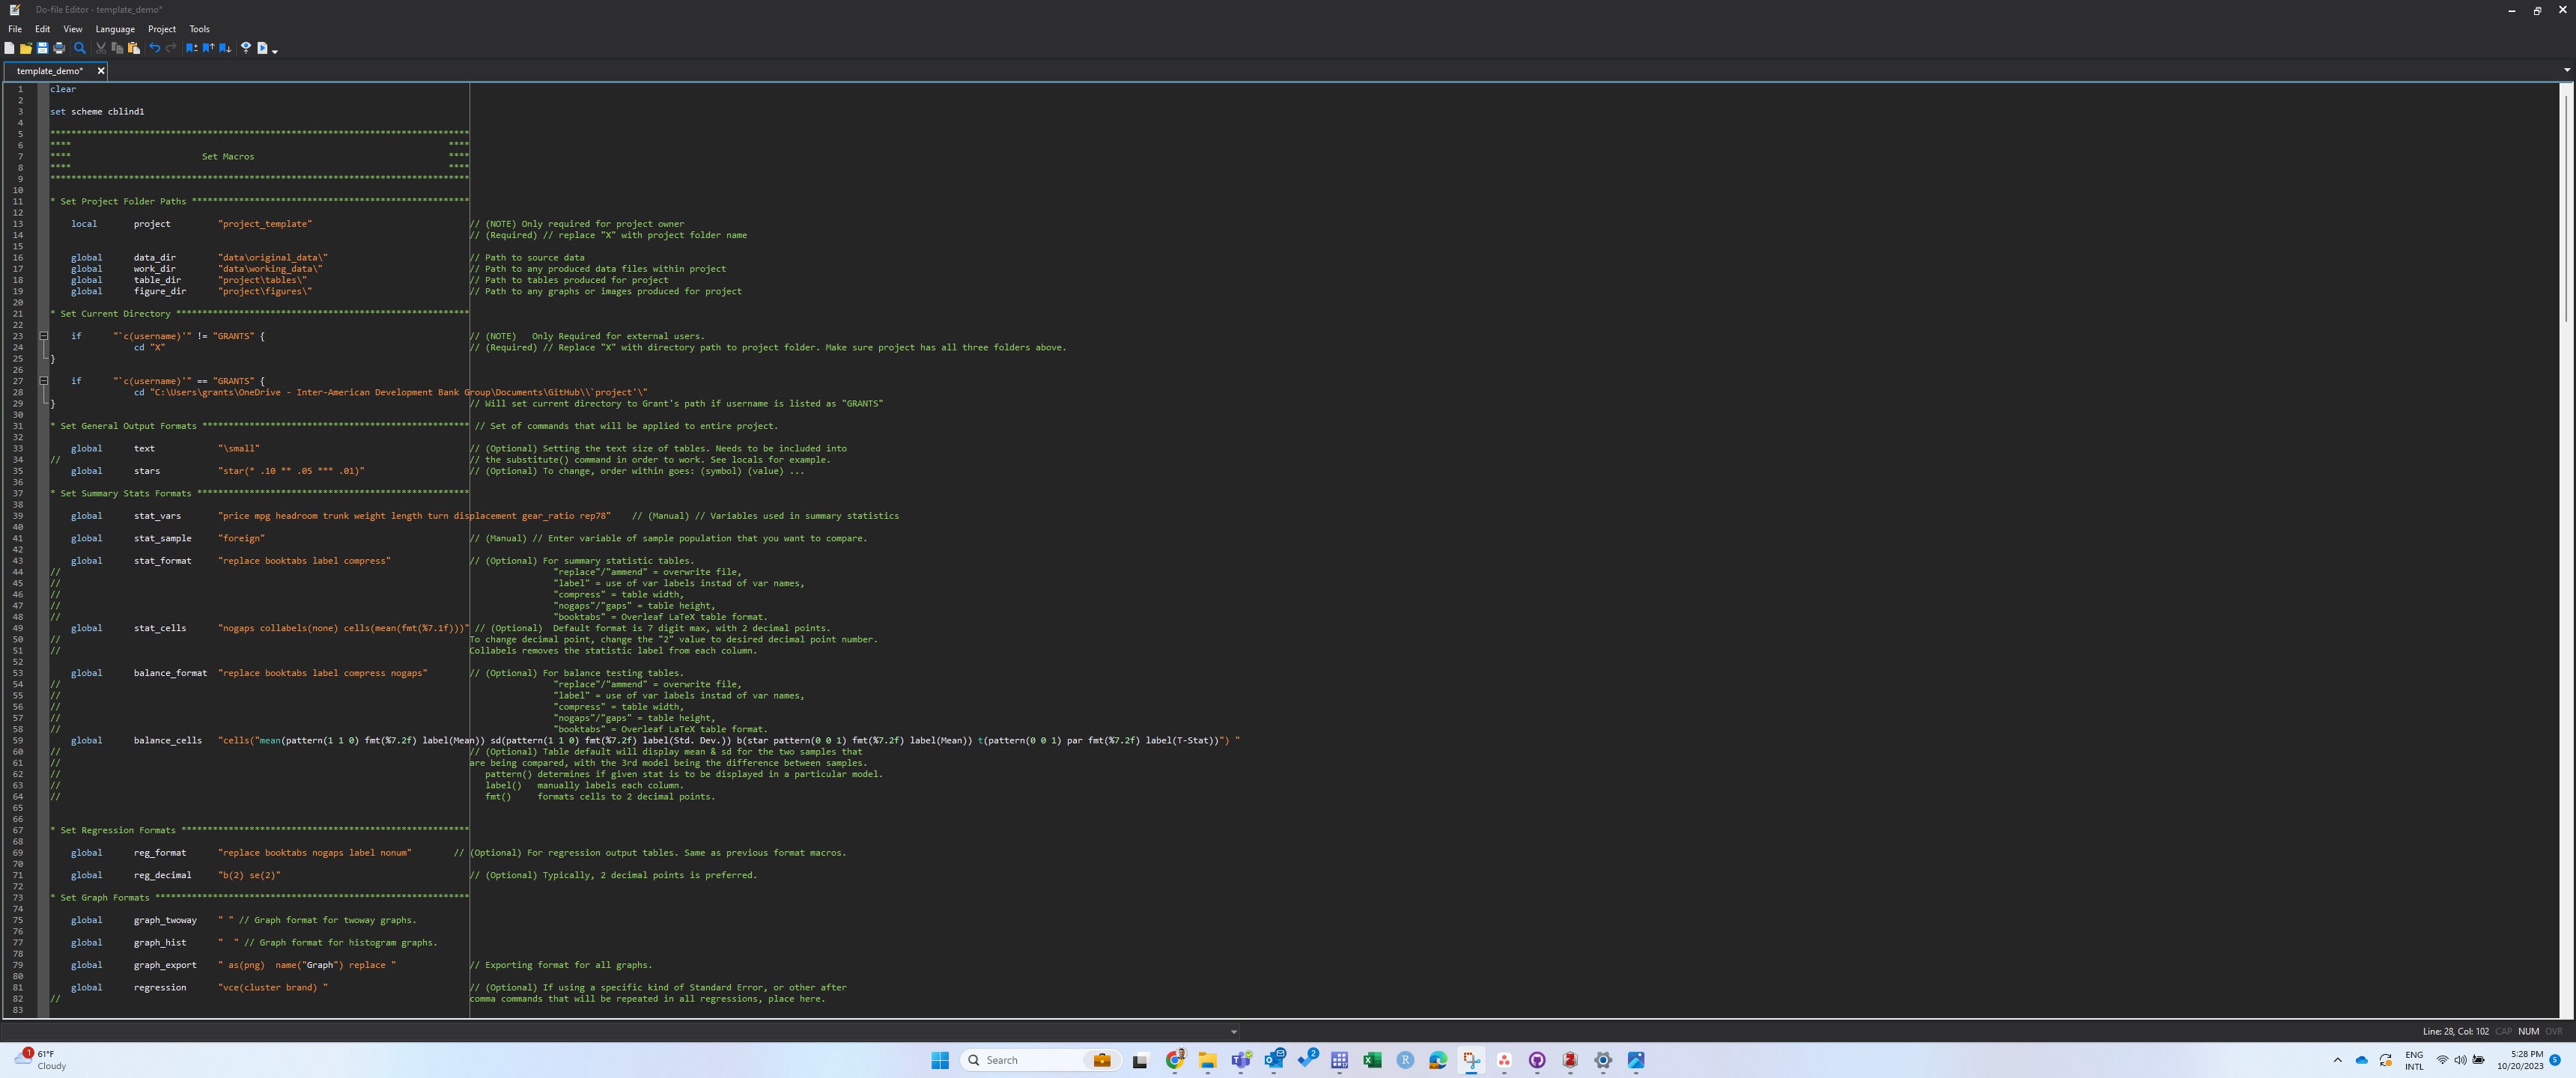
\includegraphics[width=1\textwidth]{Instructions/project_template_screenshots/project_template_14.png} \\

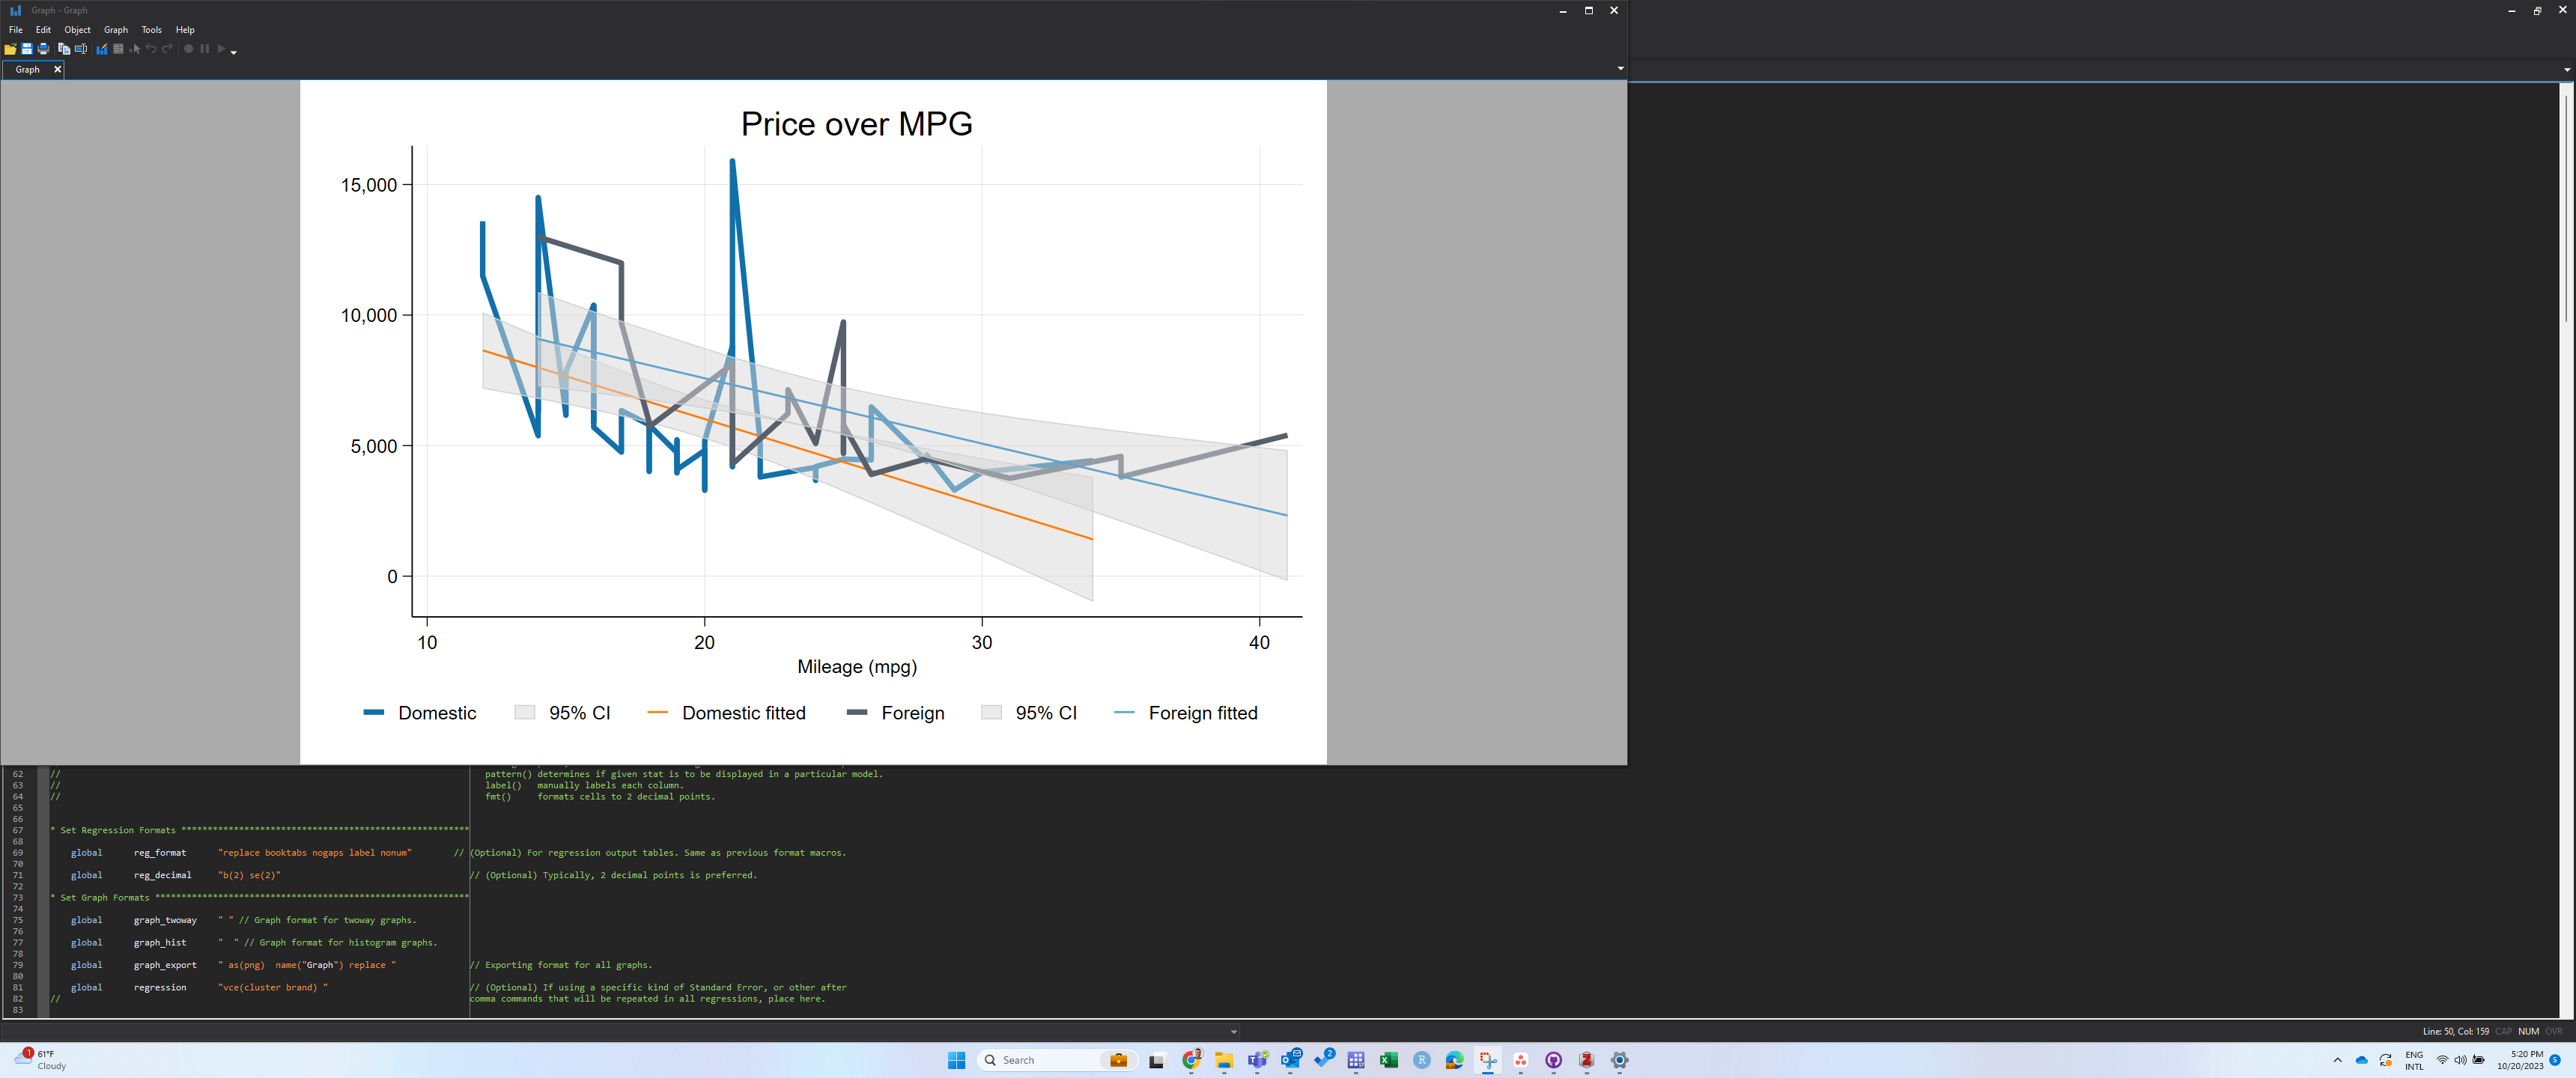
\includegraphics[width=1\textwidth]{Instructions/project_template_screenshots/project_template_15.png} \\

Now return to GitHub Desktop, and push the new tables and figures to Overleaf. \\ 

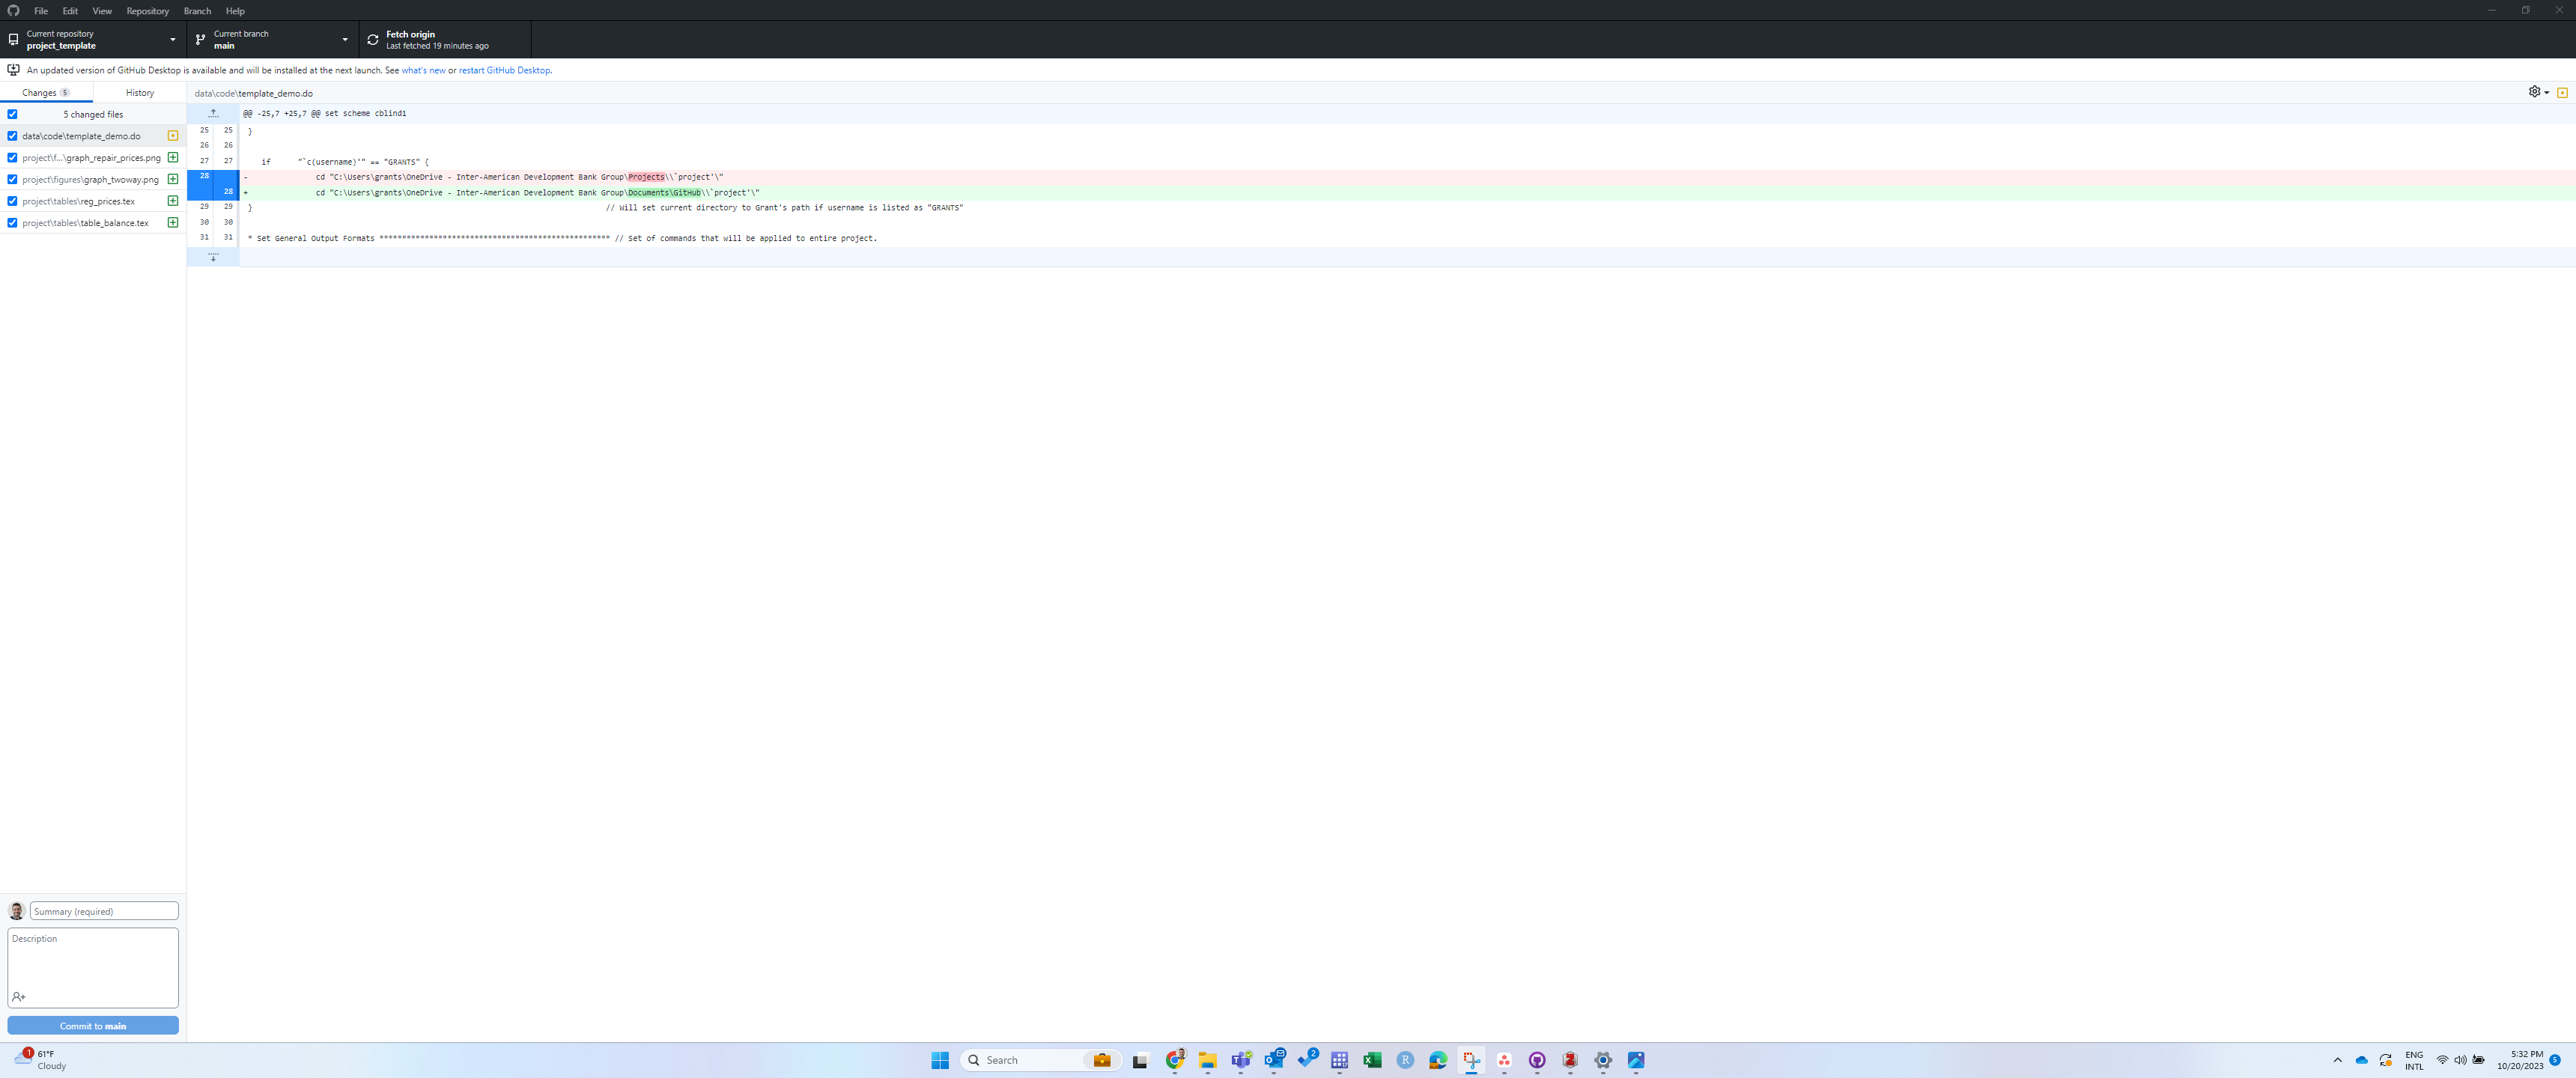
\includegraphics[width=1\textwidth]{Instructions/project_template_screenshots/project_template_16.png} \\

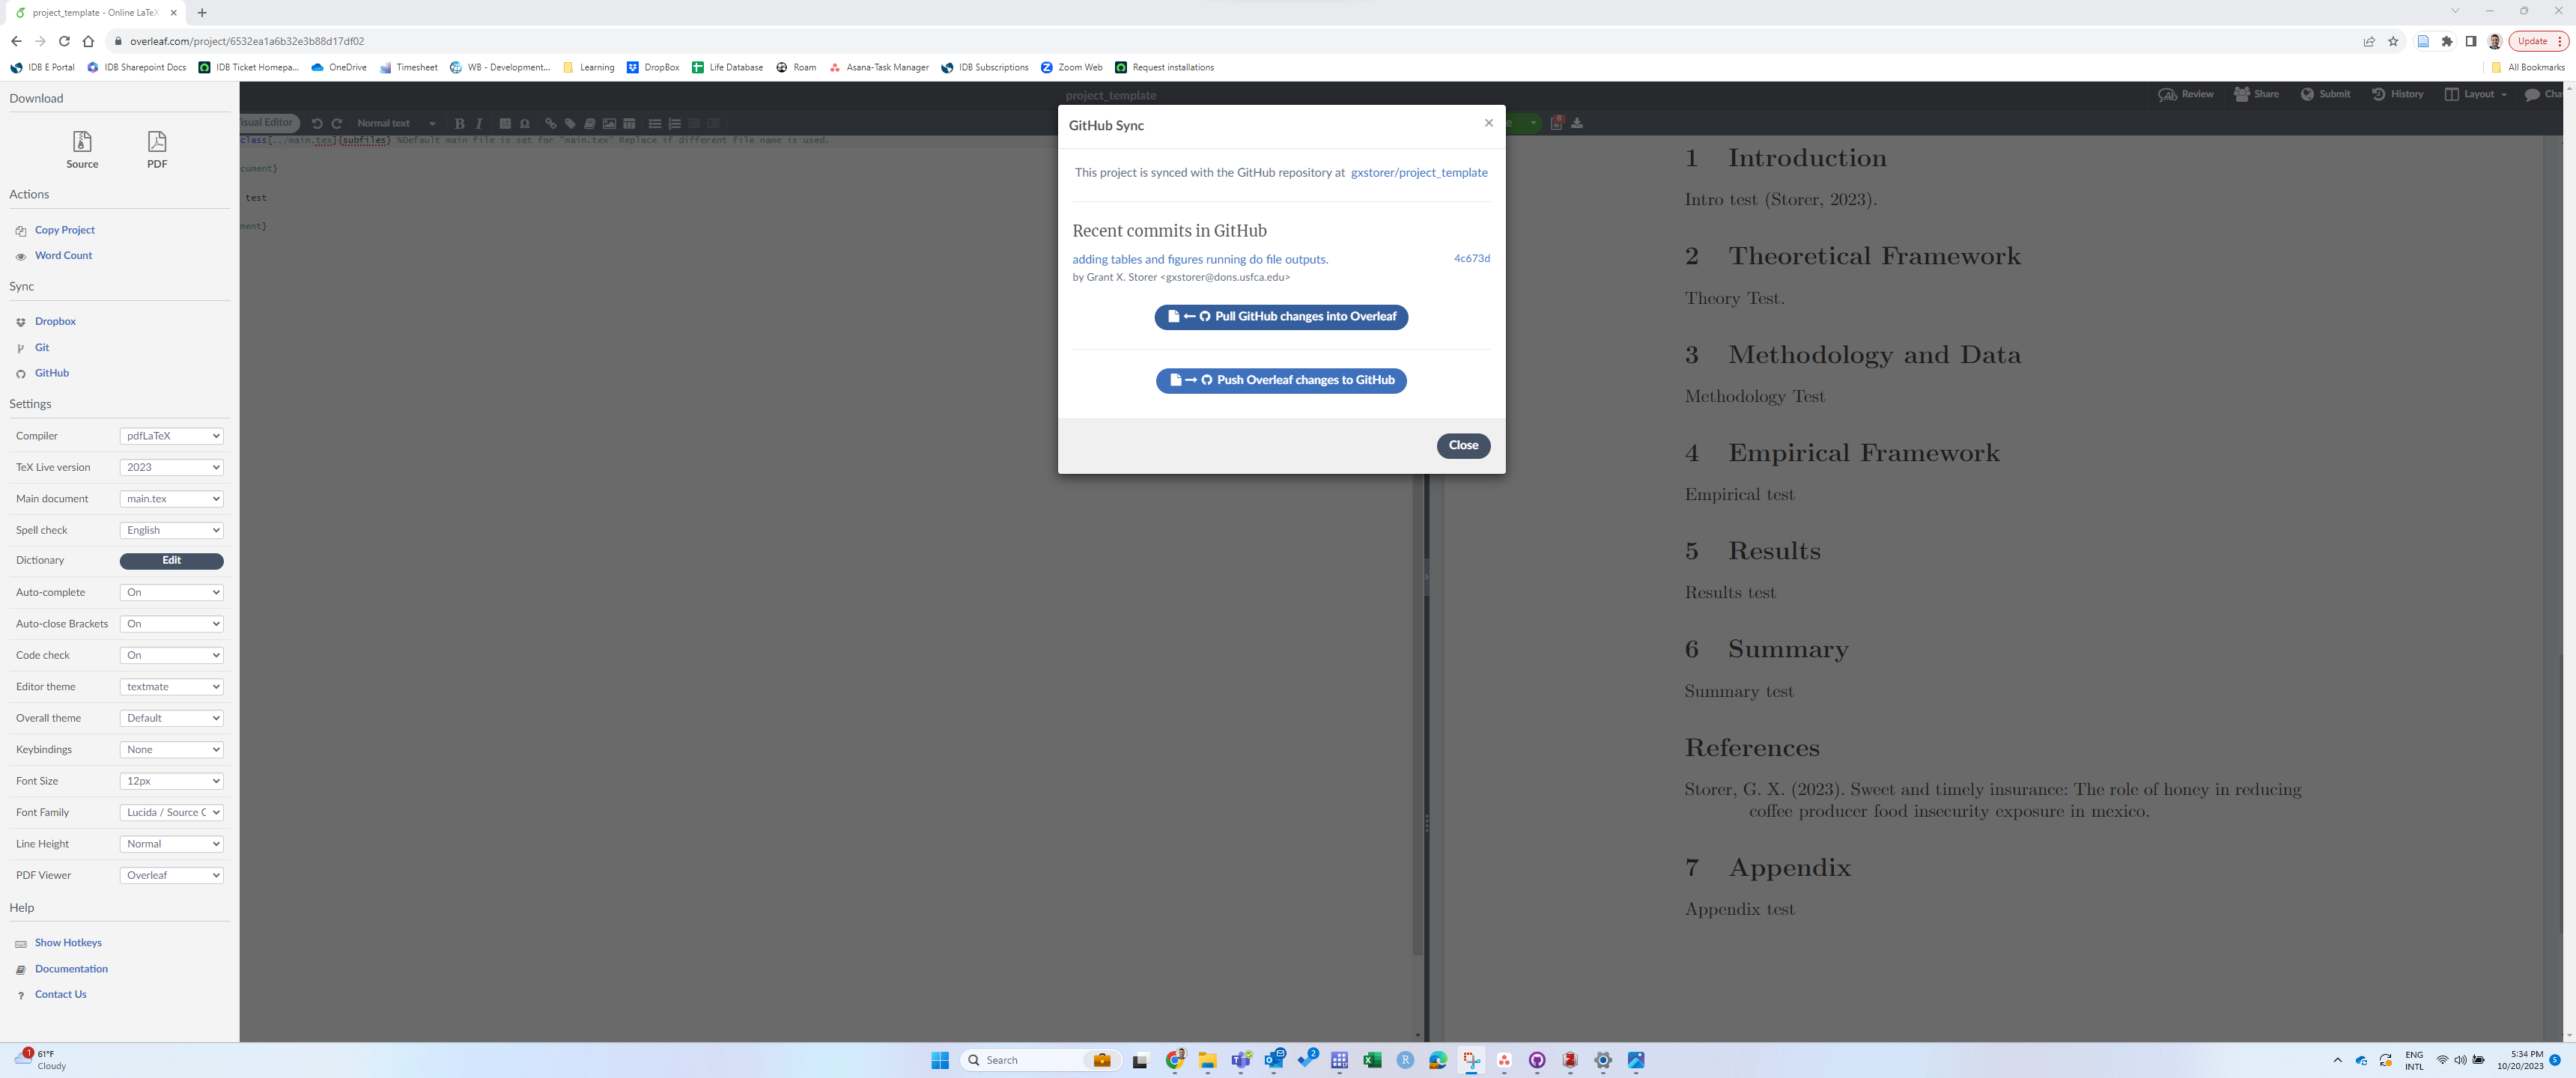
\includegraphics[width=1\textwidth]{Instructions/project_template_screenshots/project_template_17.png} \\

The new tables and figures can now be found in the project folders, and are available to be included into the paper. Use the \textbf{include} commands within the given section that you want to place these elements within the paper. For this example, I'll just include all 4 elements in the \textbf{5\_results} section. \\

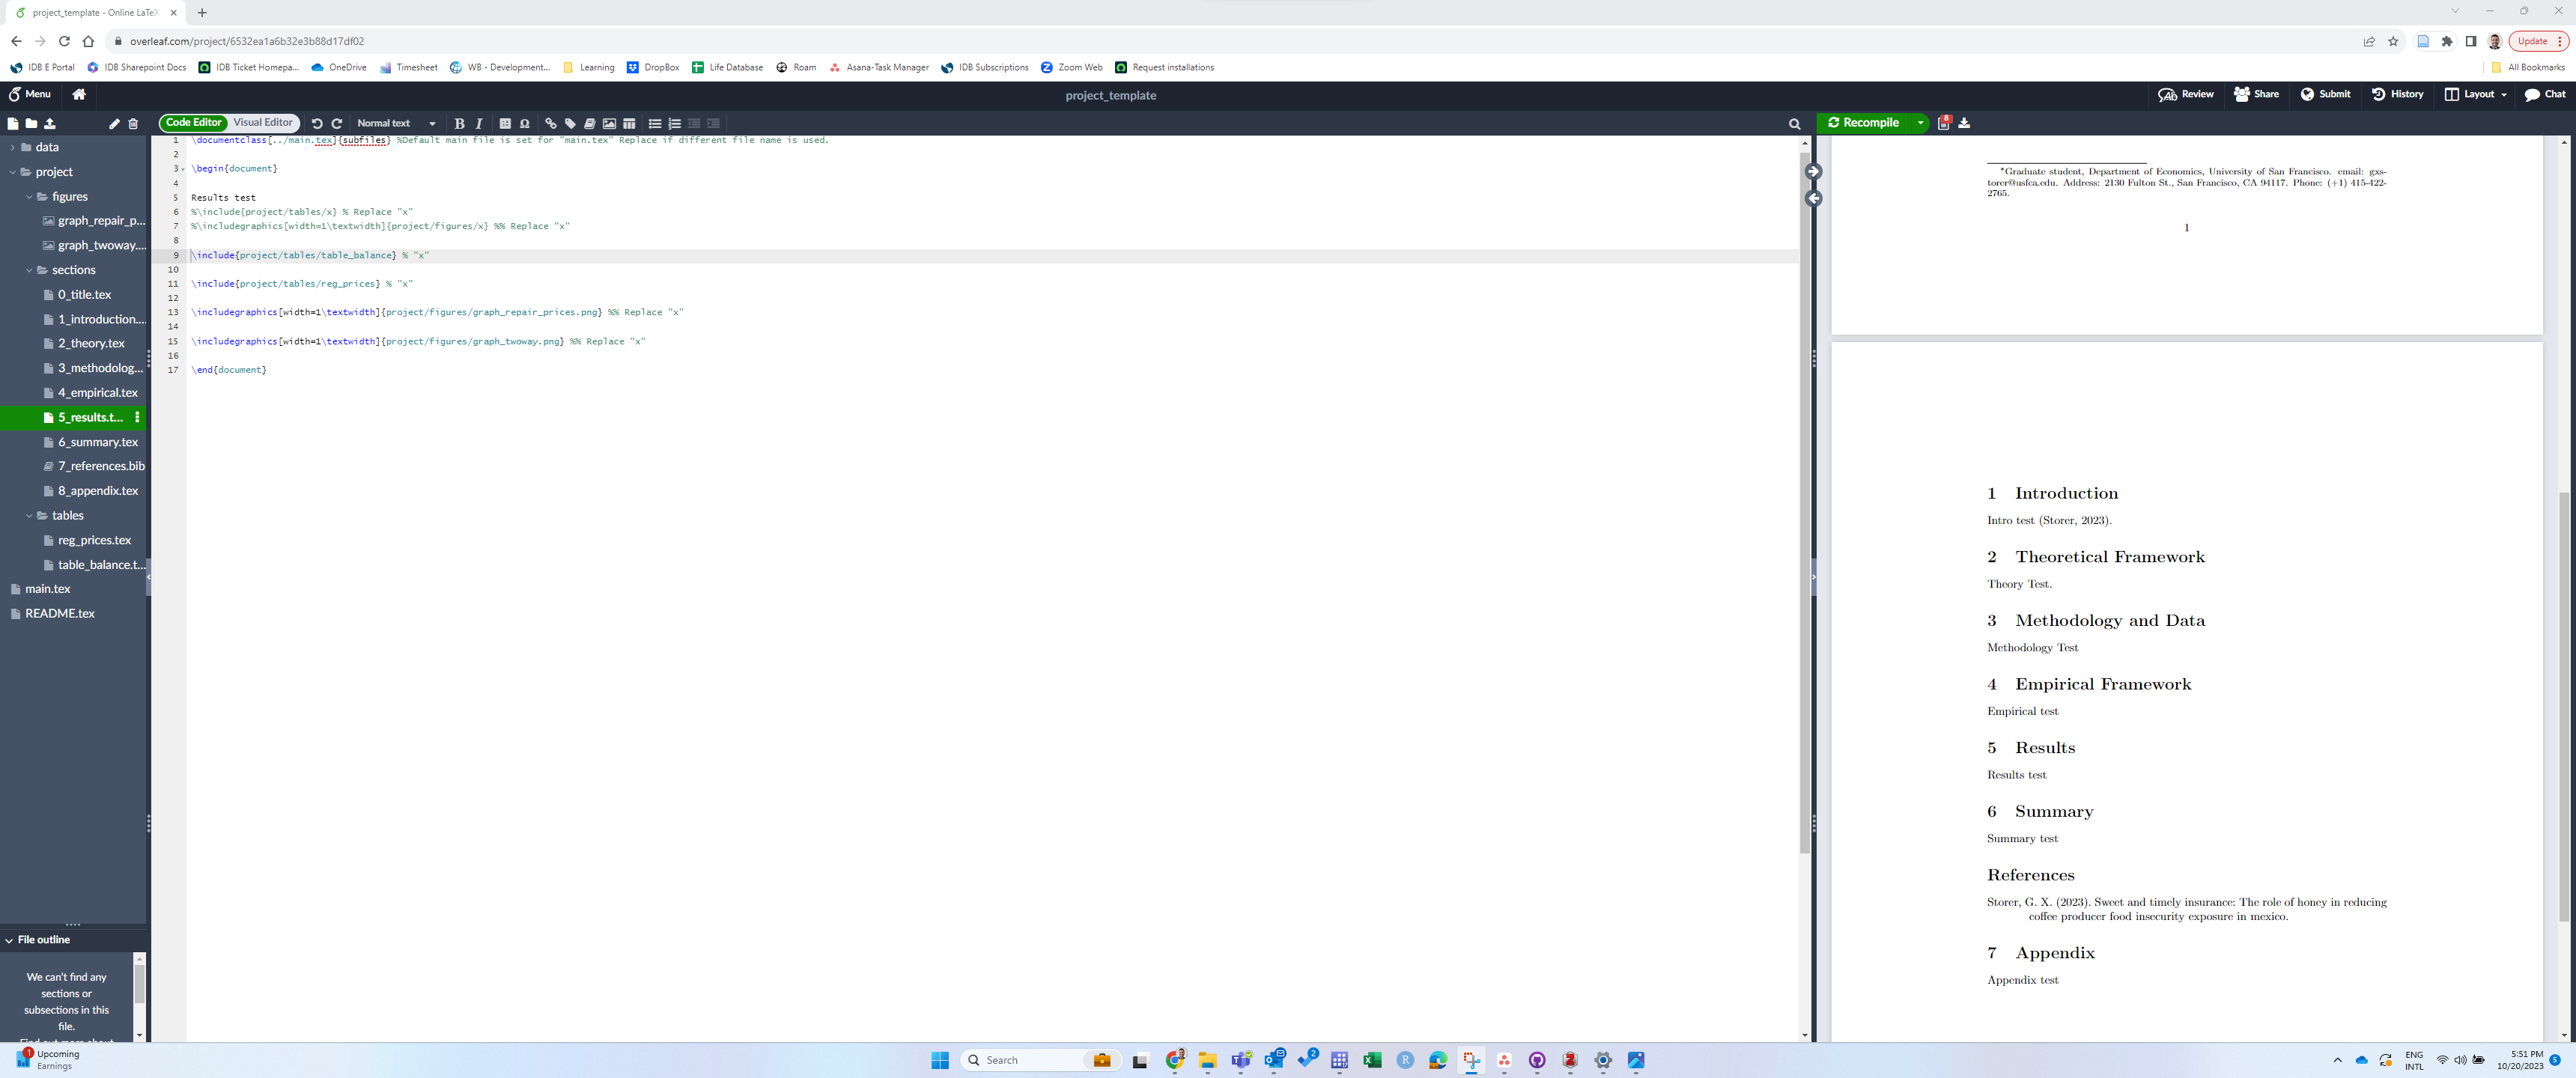
\includegraphics[width=1\textwidth]{Instructions/project_template_screenshots/project_template_18.png} \\

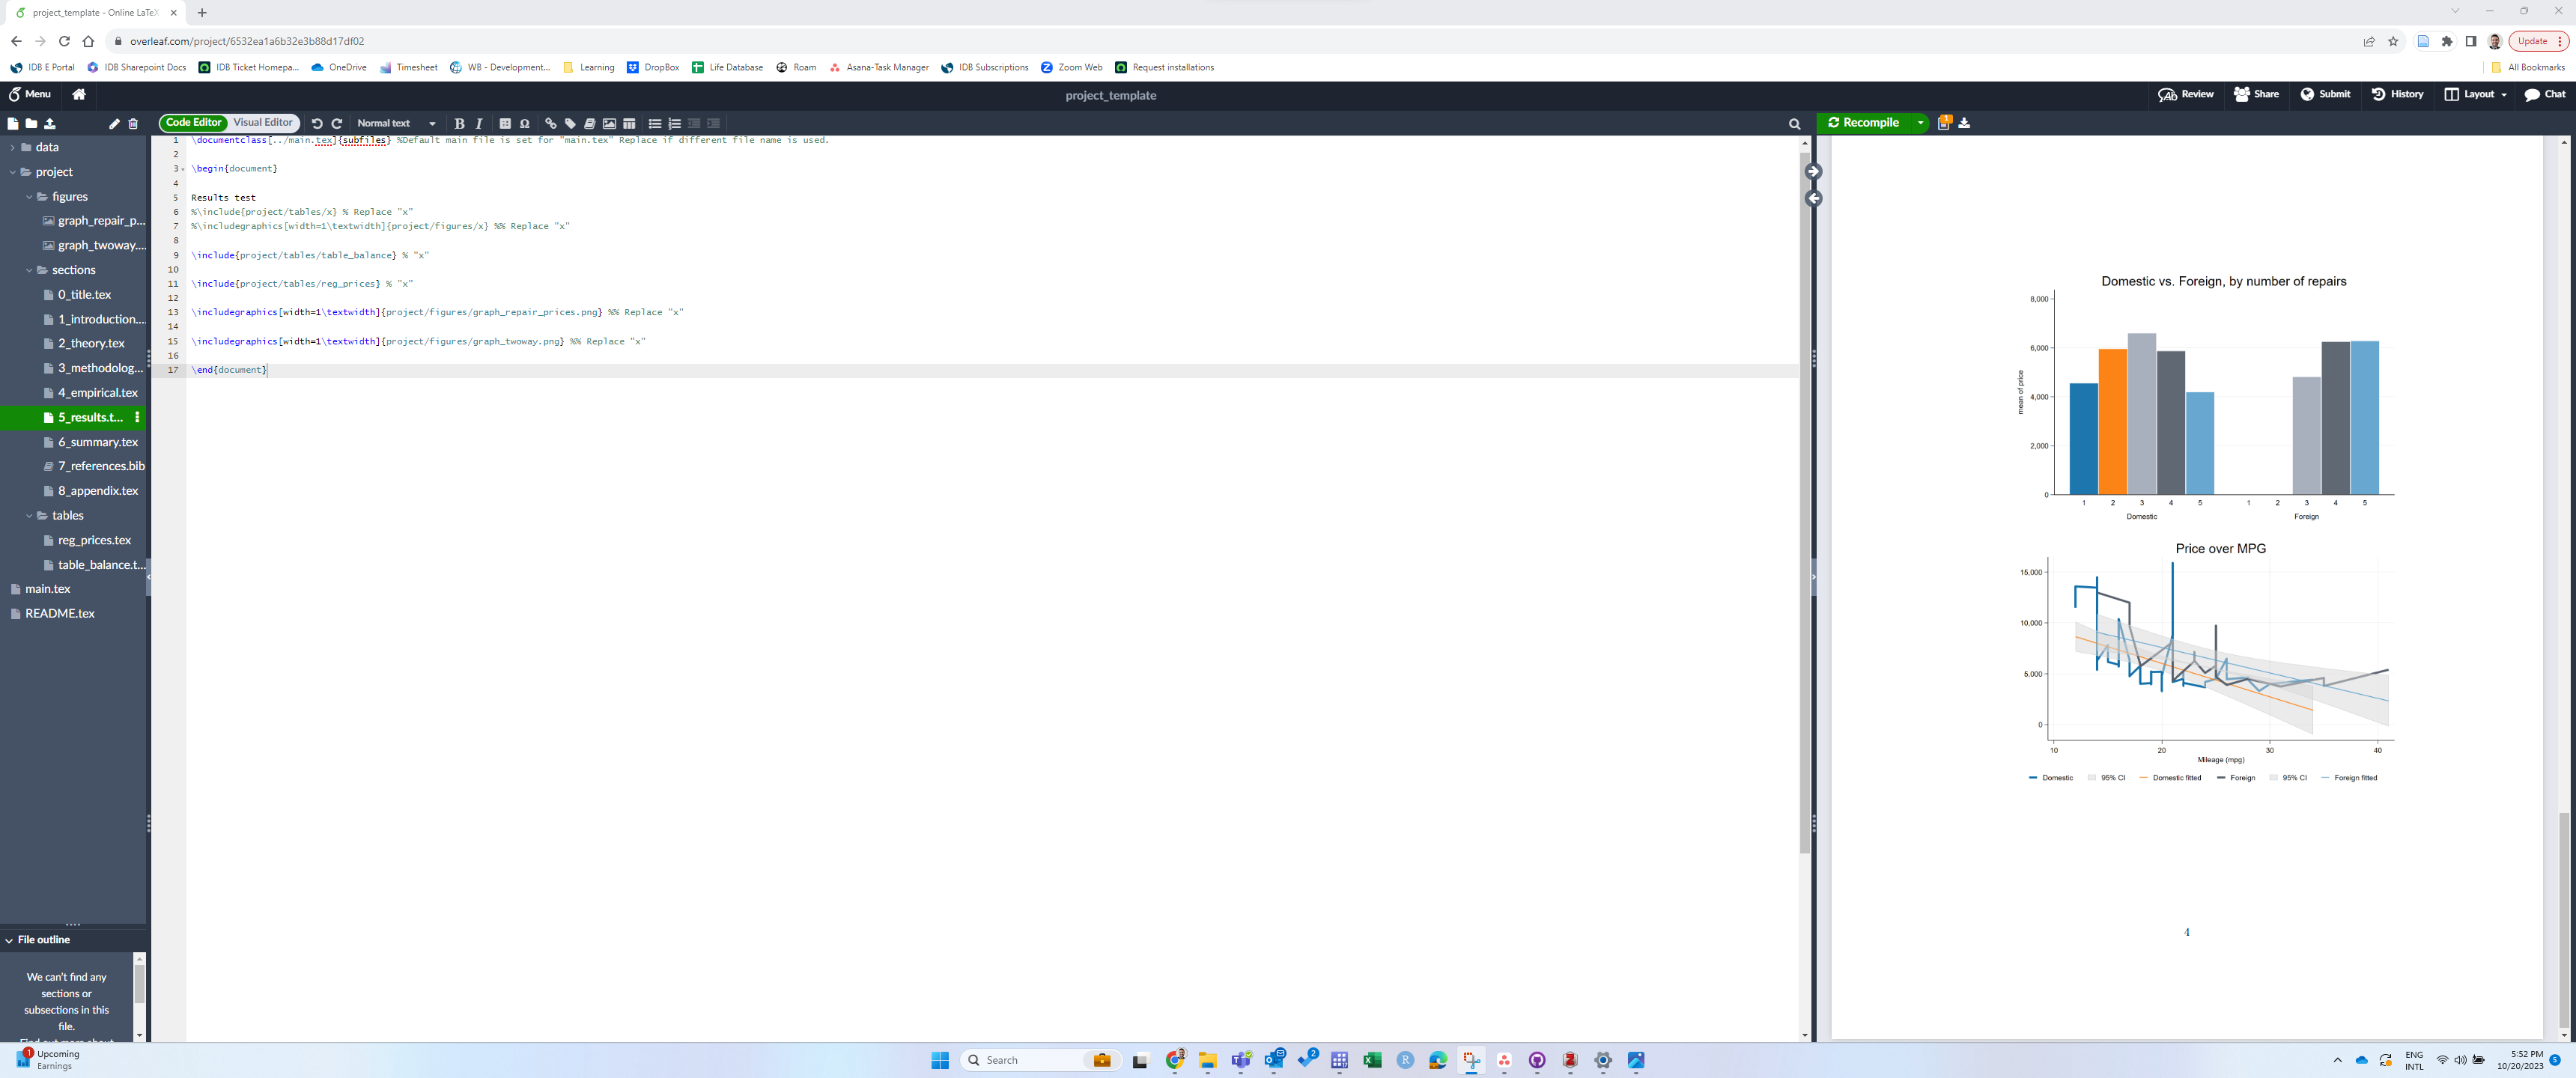
\includegraphics[width=1\textwidth]{Instructions/project_template_screenshots/project_template_19.png} \\

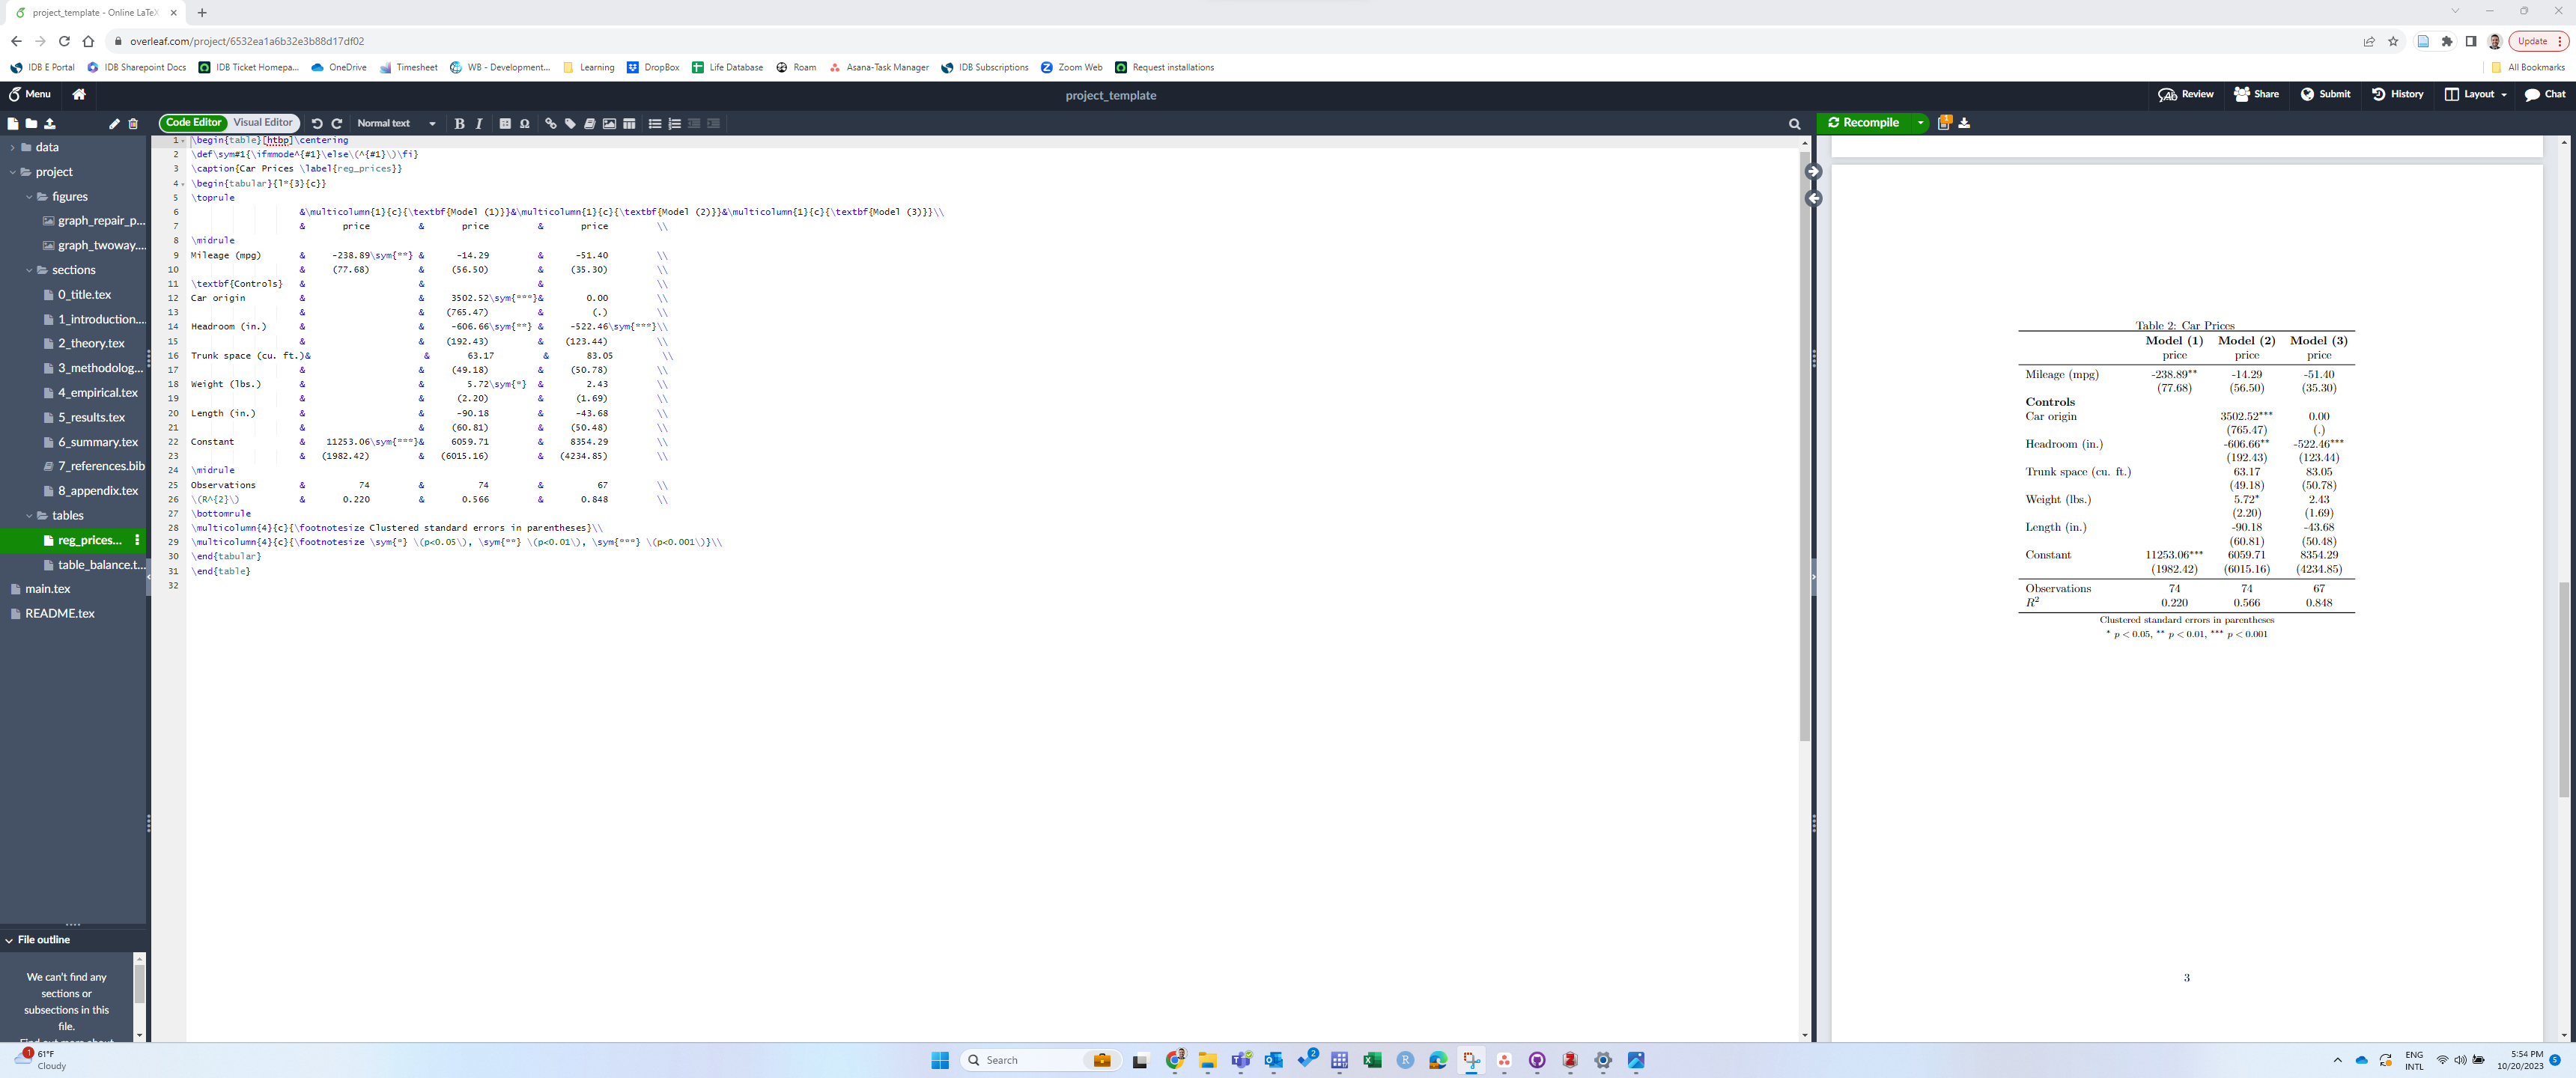
\includegraphics[width=1\textwidth]{Instructions/project_template_screenshots/project_template_20.png} \\

\section{Editing Outputs}

One most beneficial aspects of using GitHub is making changes to outputs doesn't have to be completely disrupt the format of your working paper. For instance, what if you were working on the regression about fuel efficiency's relationship to car prices, and you decide that instead of using the control variable \textbf{length}, you want to instead use \textbf{gear\_ratio}. Just go into the do-file, replace length with gear\_ratio, and run the do-file. After saving the changes, go into GitHub Desktop and push the changes to Overleaf. \\

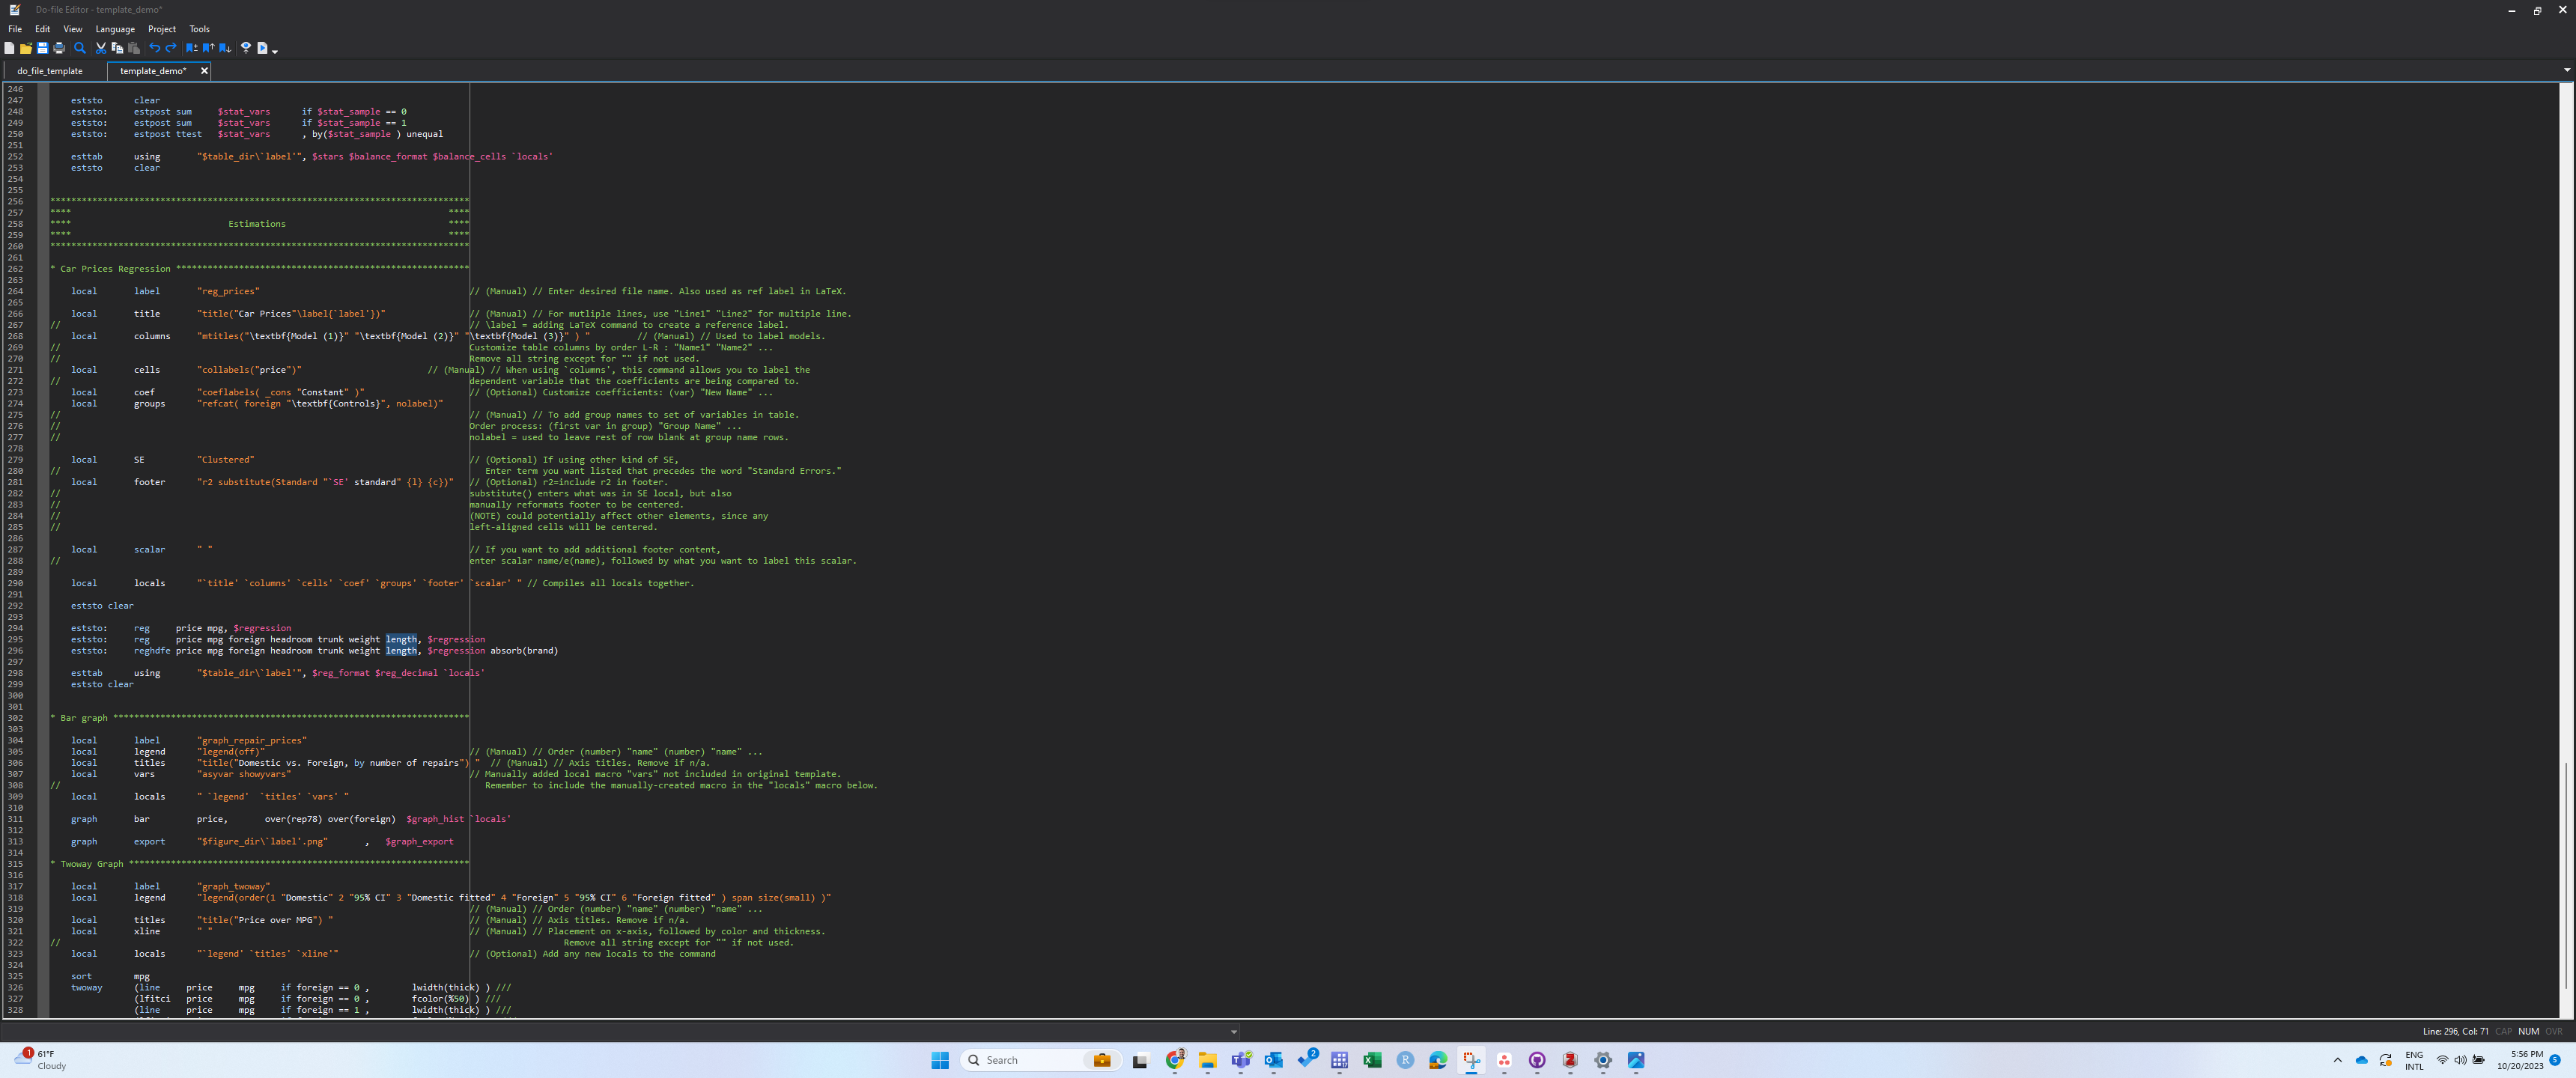
\includegraphics[width=1\textwidth]{Instructions/project_template_screenshots/project_template_21.png} \\

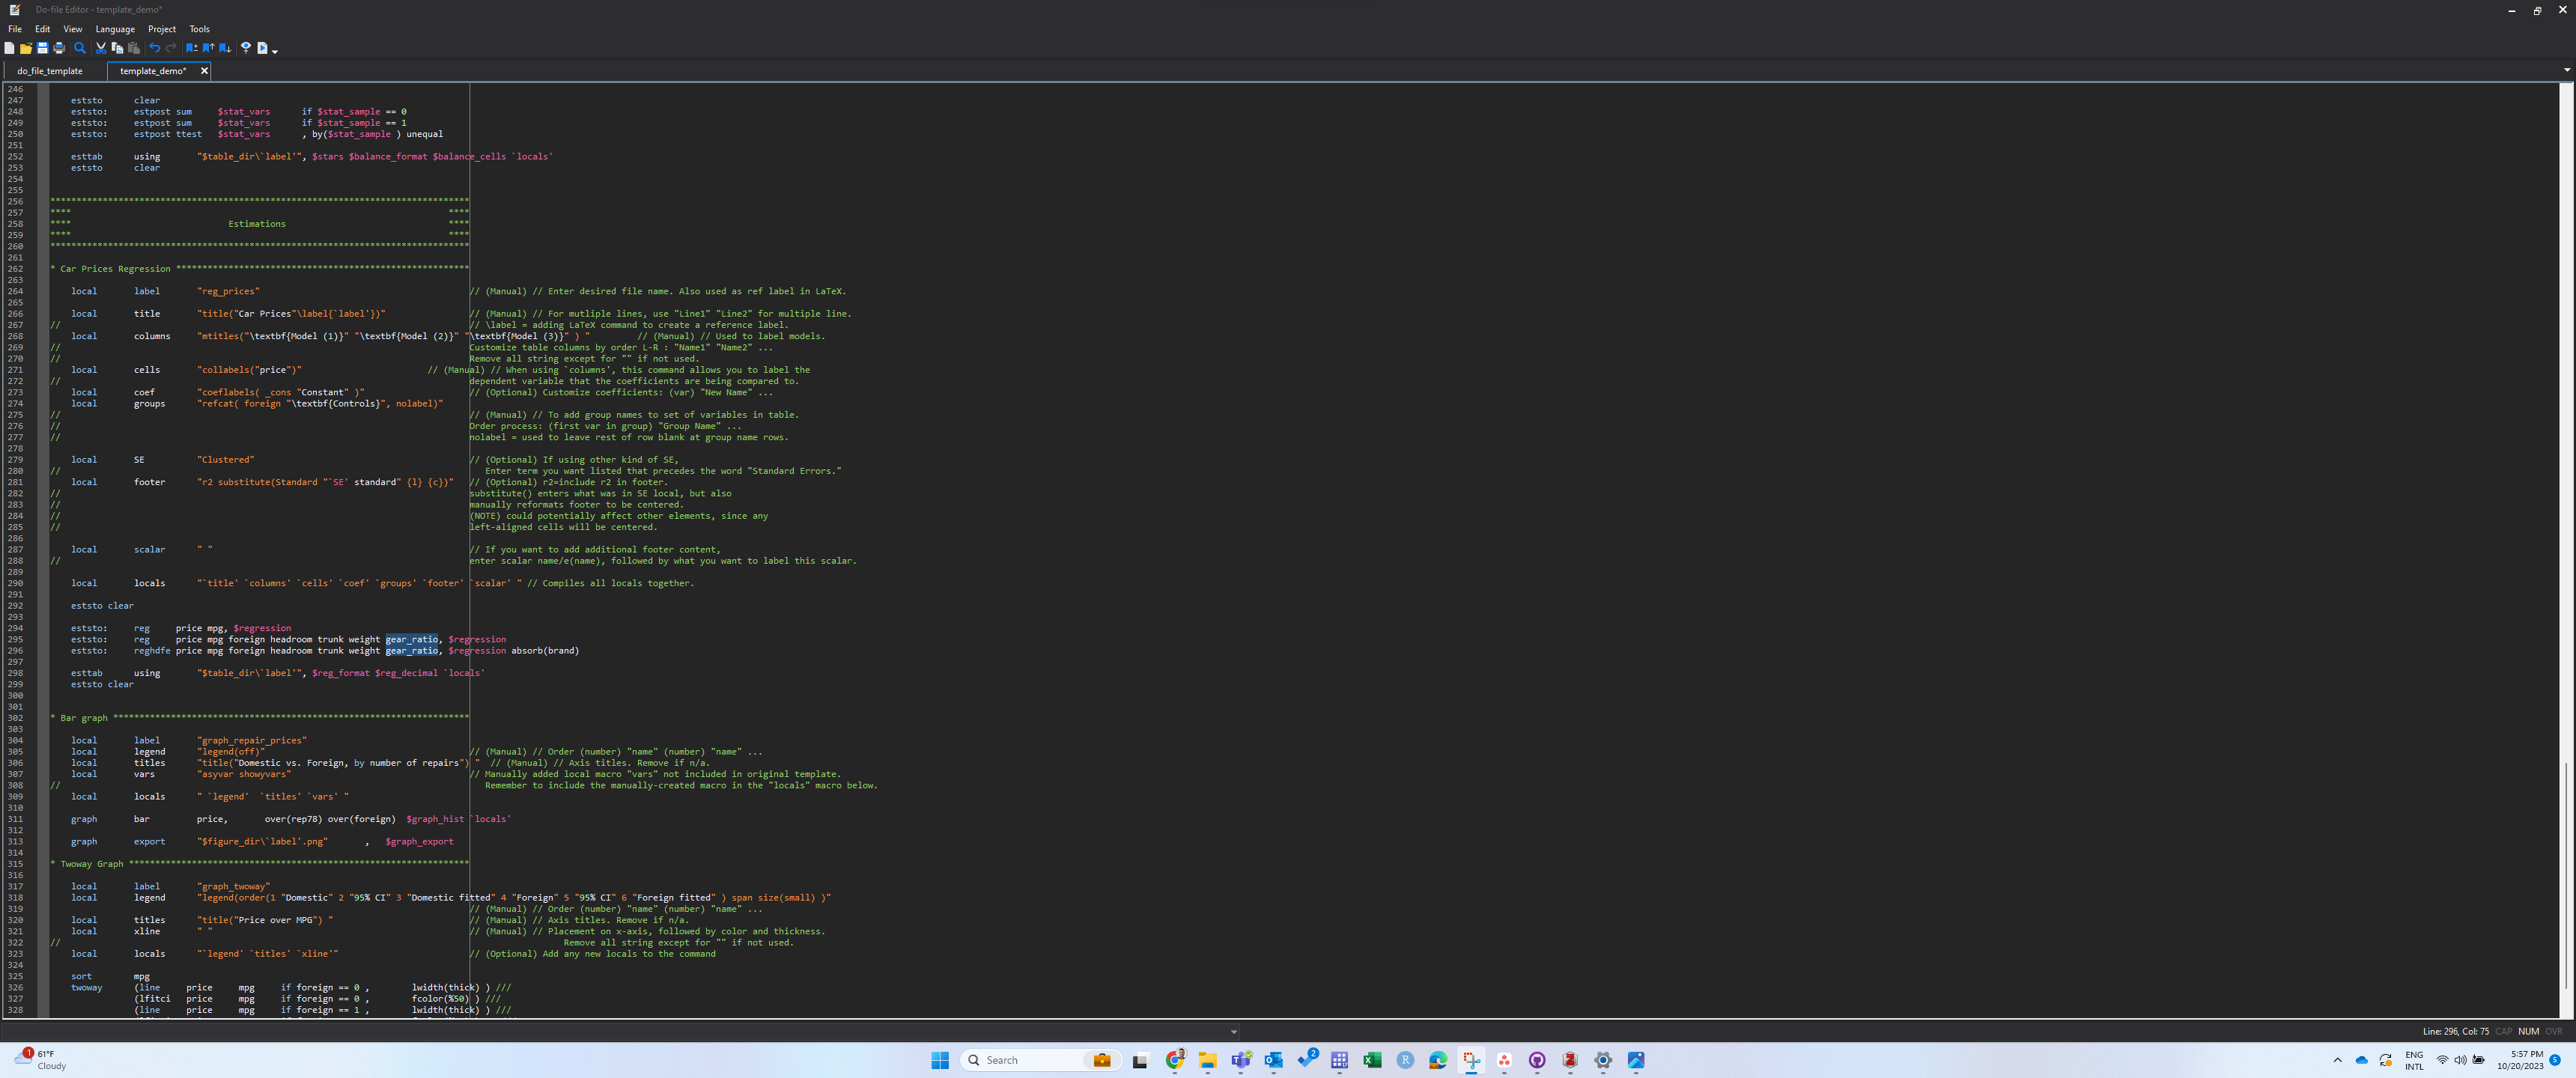
\includegraphics[width=1\textwidth]{Instructions/project_template_screenshots/project_template_22.png} \\

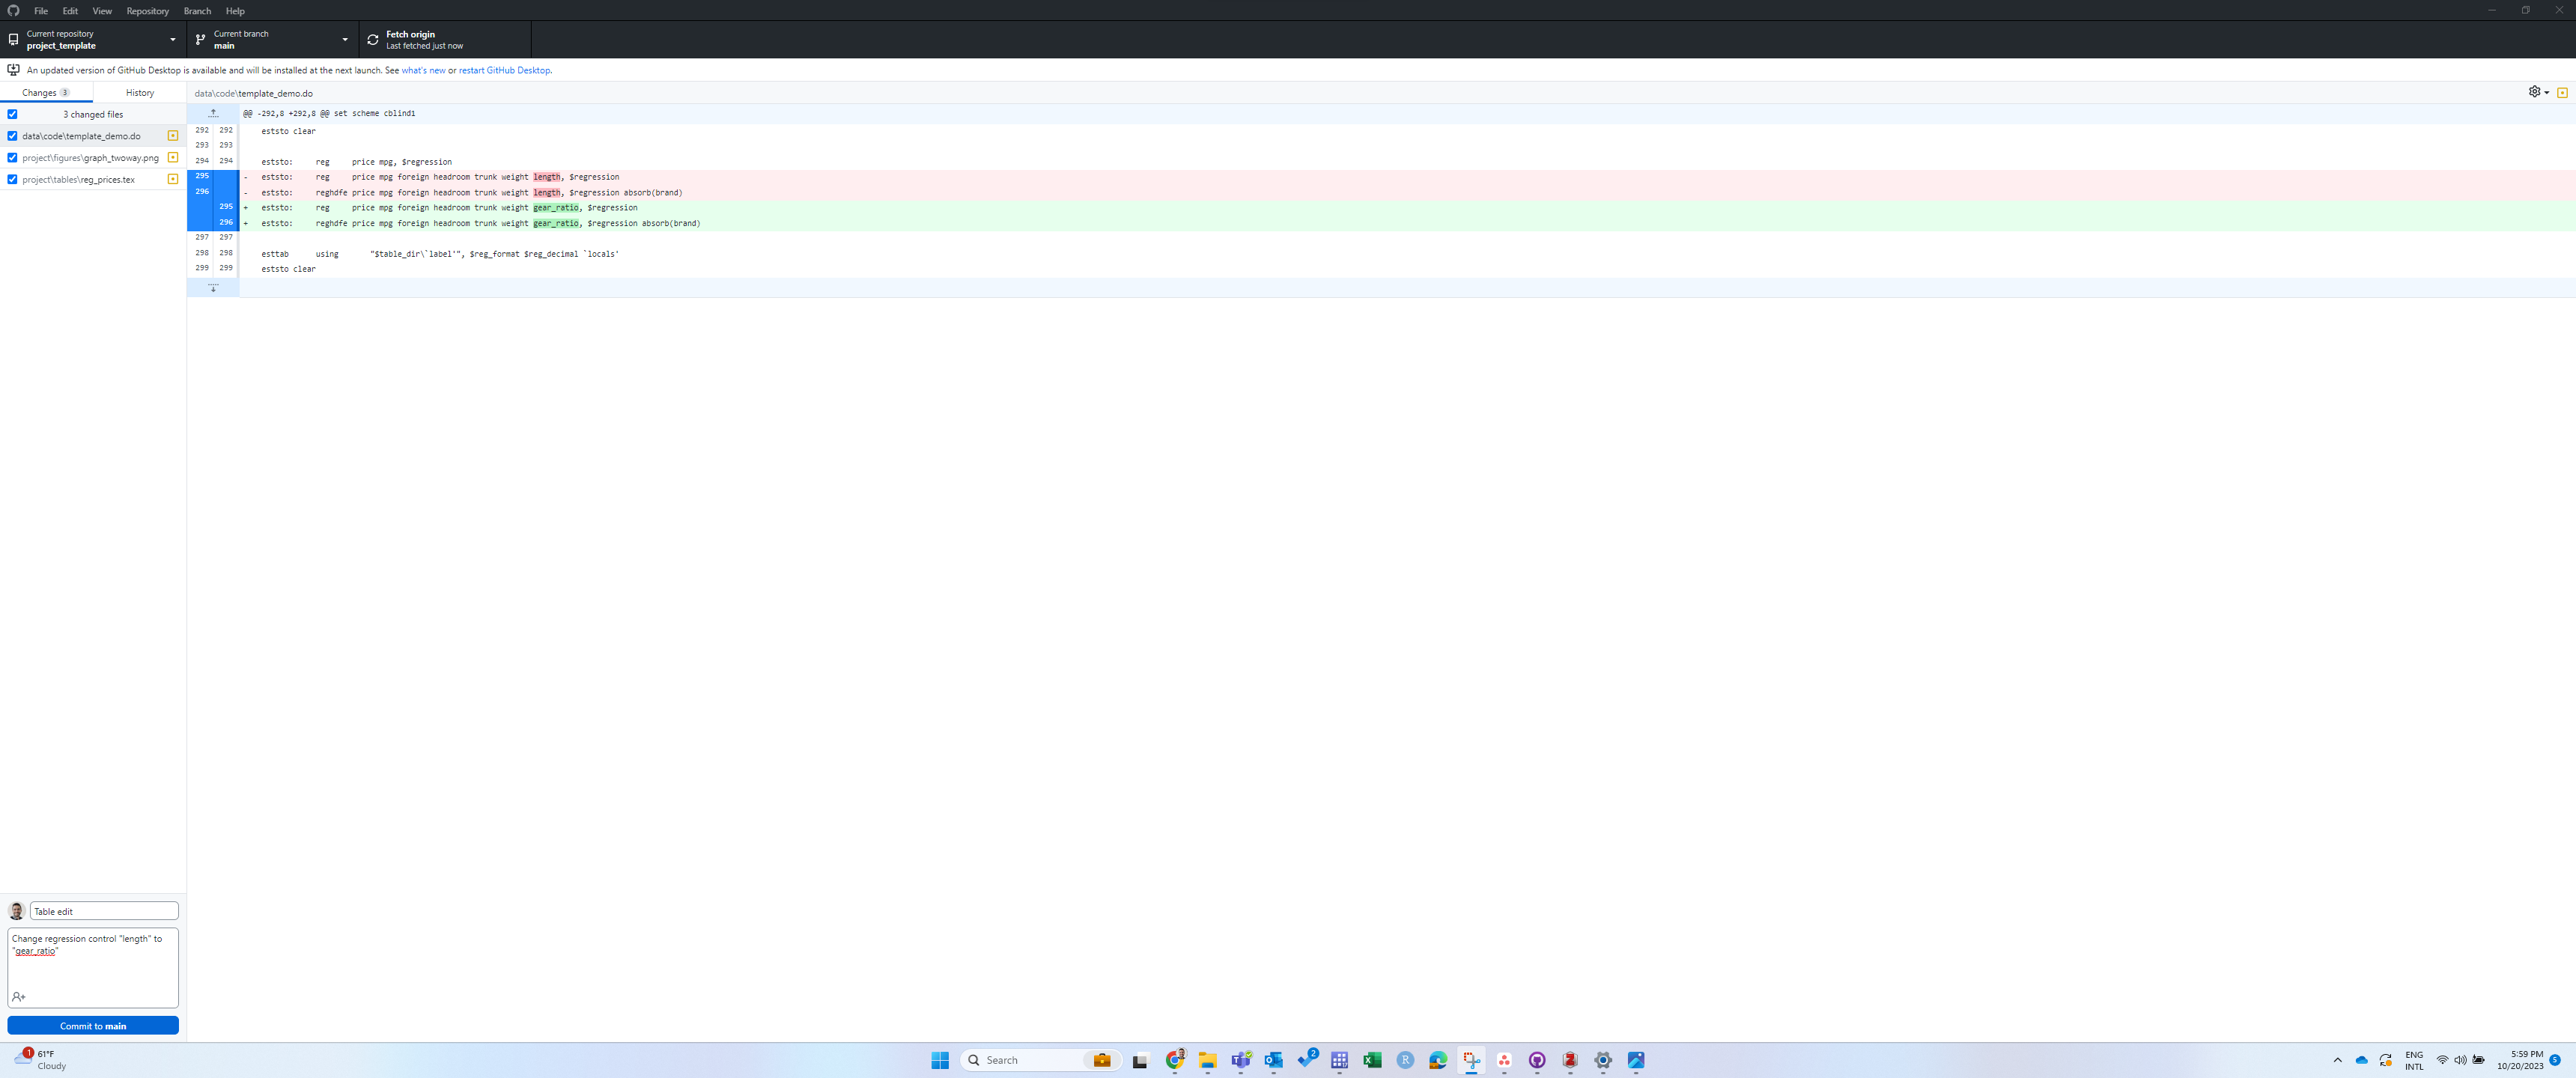
\includegraphics[width=1\textwidth]{Instructions/project_template_screenshots/project_template_23.png} \\

Return to Overleaf, and pull the changes. You'll see that difference between the following two images, that the only change is the control of length is now producing the coefficient for the control for gear\_ratio. This isn't compiled yet, and so on the right pane the change isn't displayed yet, but in the third image, the changes are compiled and the new table change has been made while the format has been preserved. \\

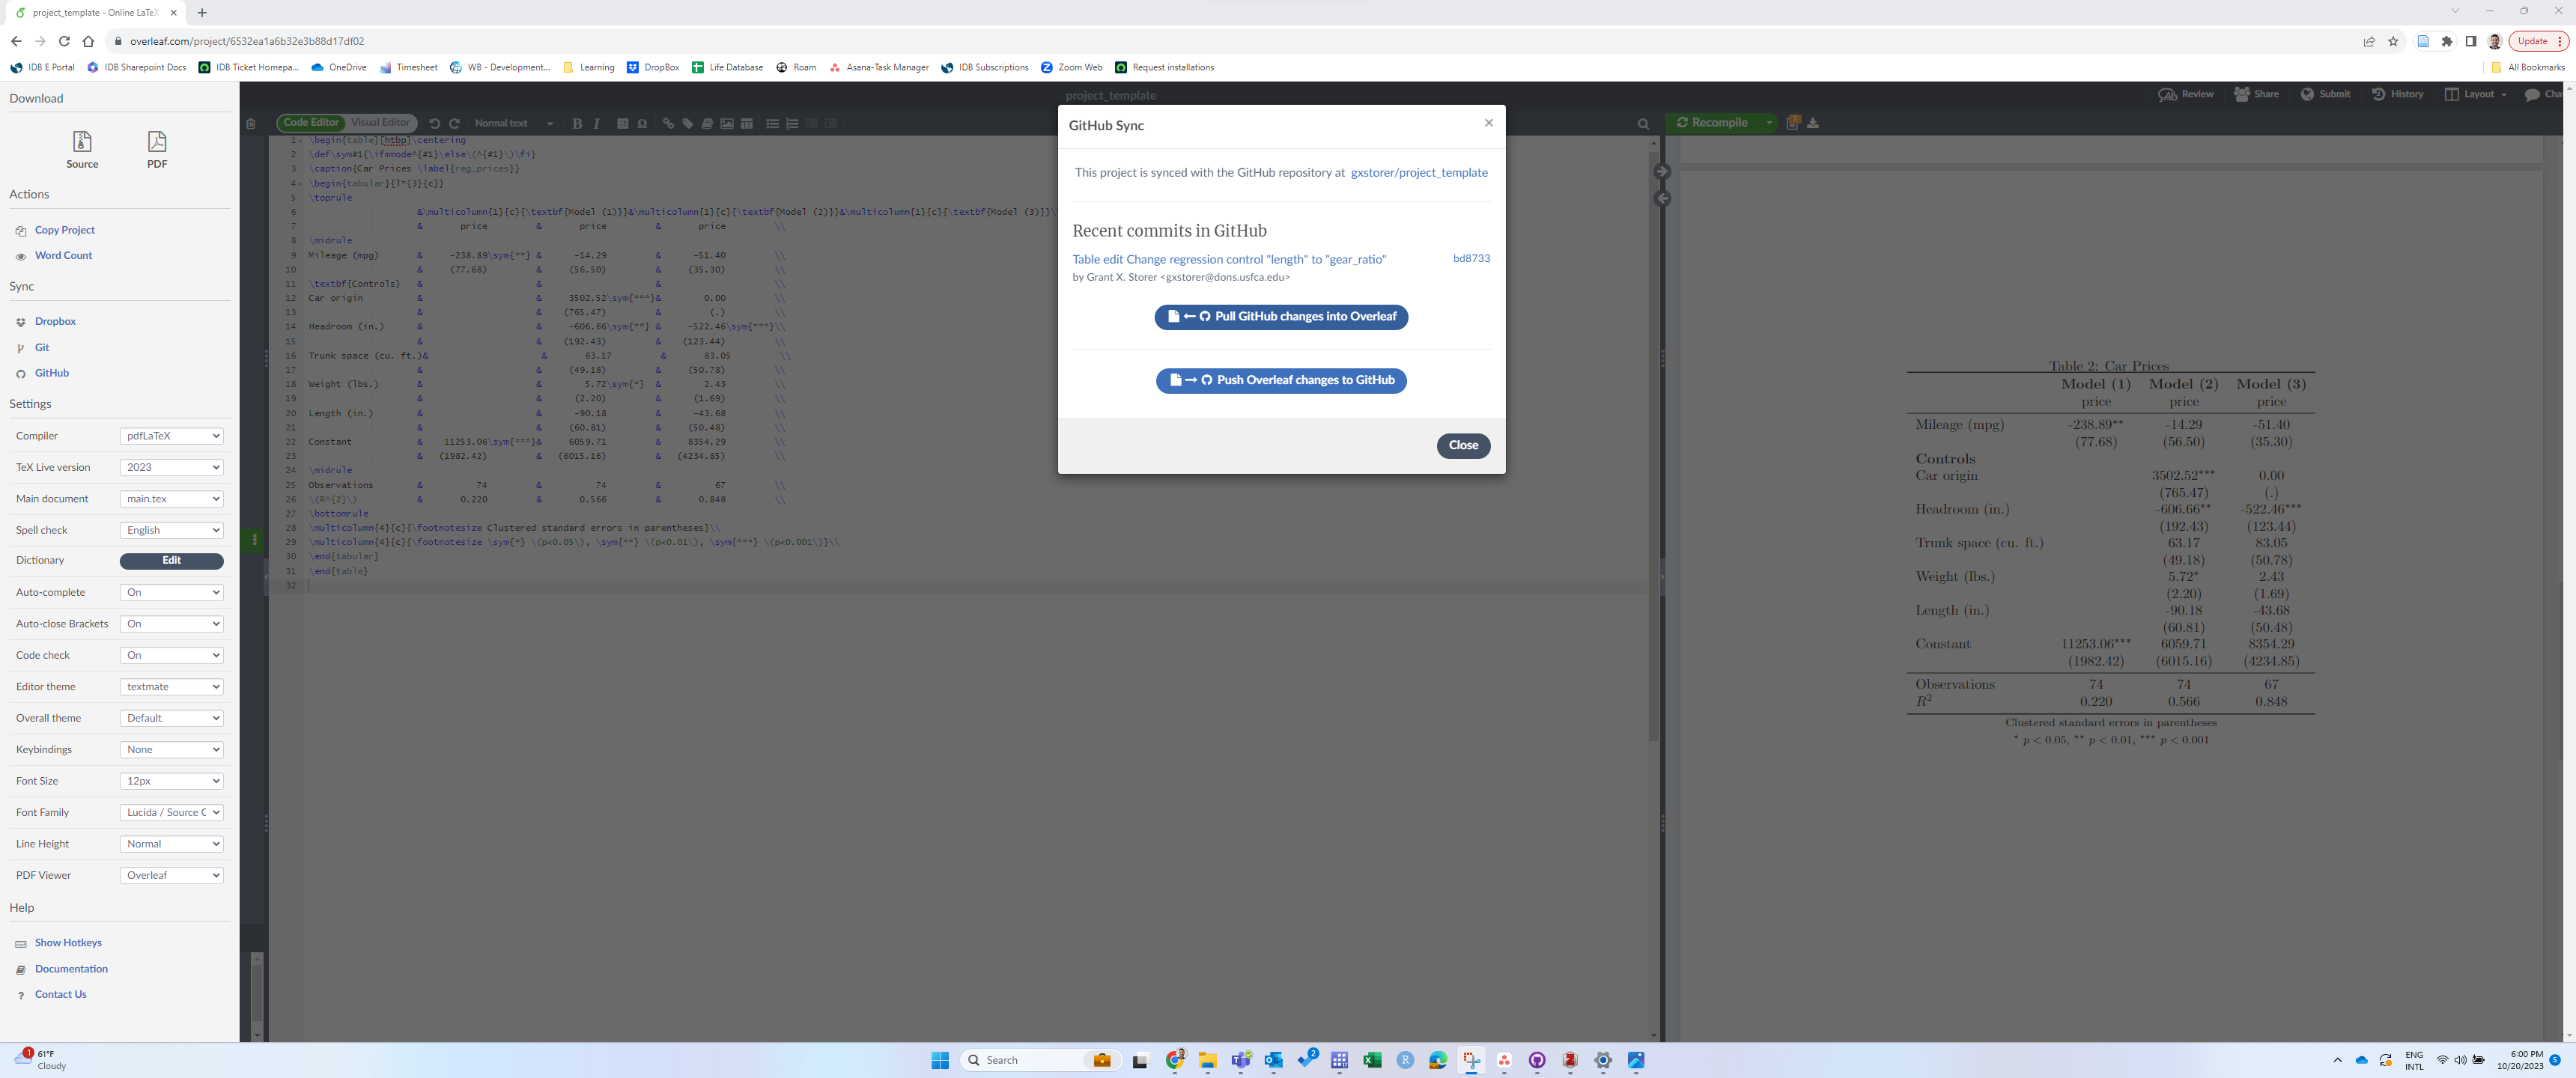
\includegraphics[width=1\textwidth]{Instructions/project_template_screenshots/project_template_24.png} \\

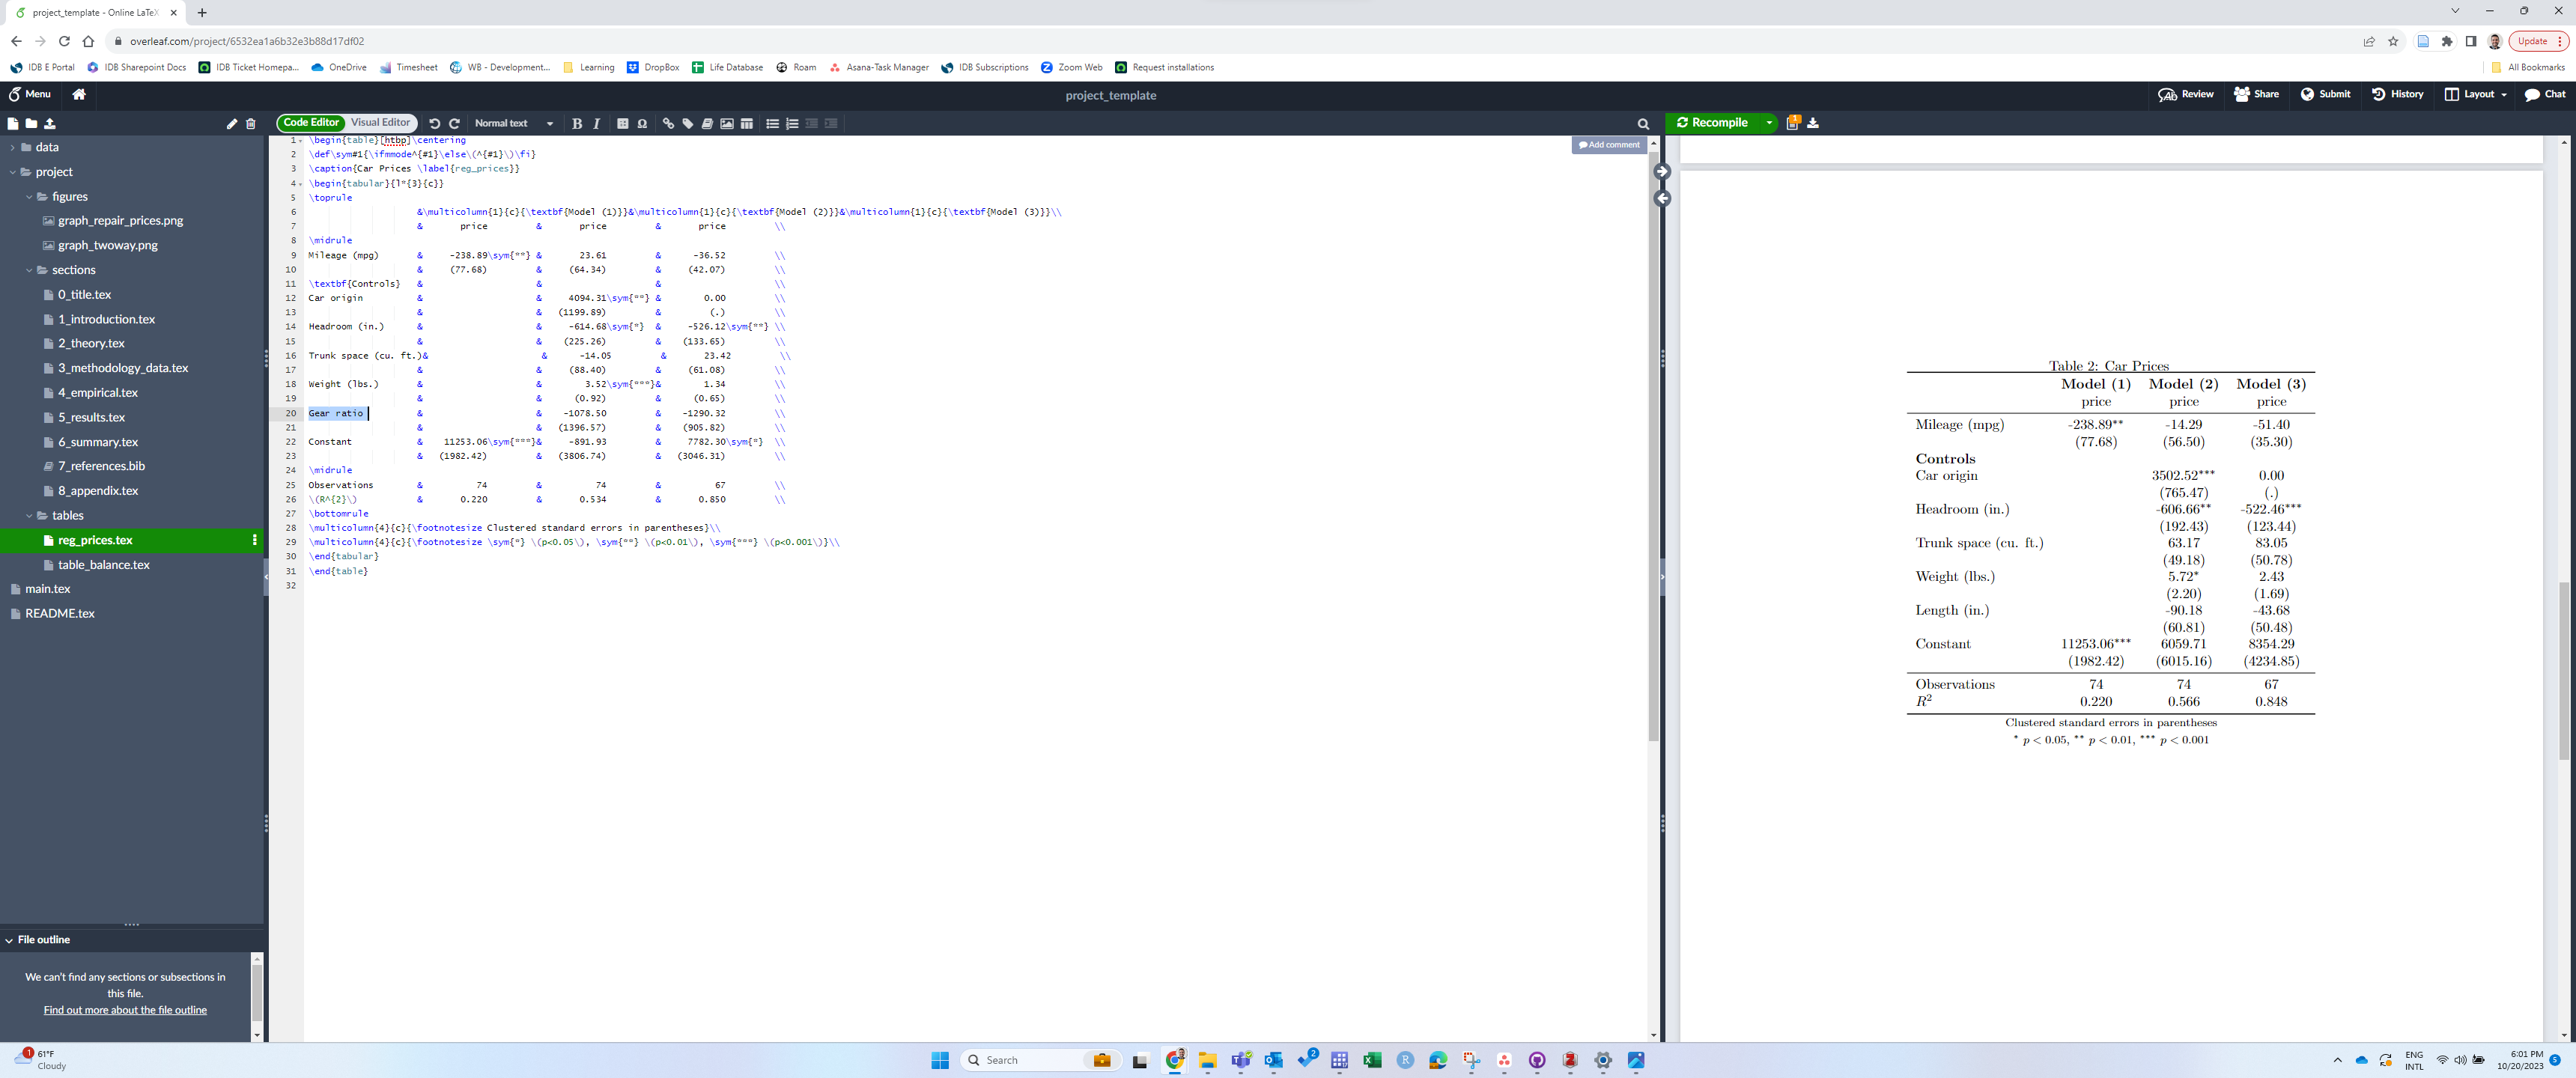
\includegraphics[width=1\textwidth]{Instructions/project_template_screenshots/project_template_25.png} \\

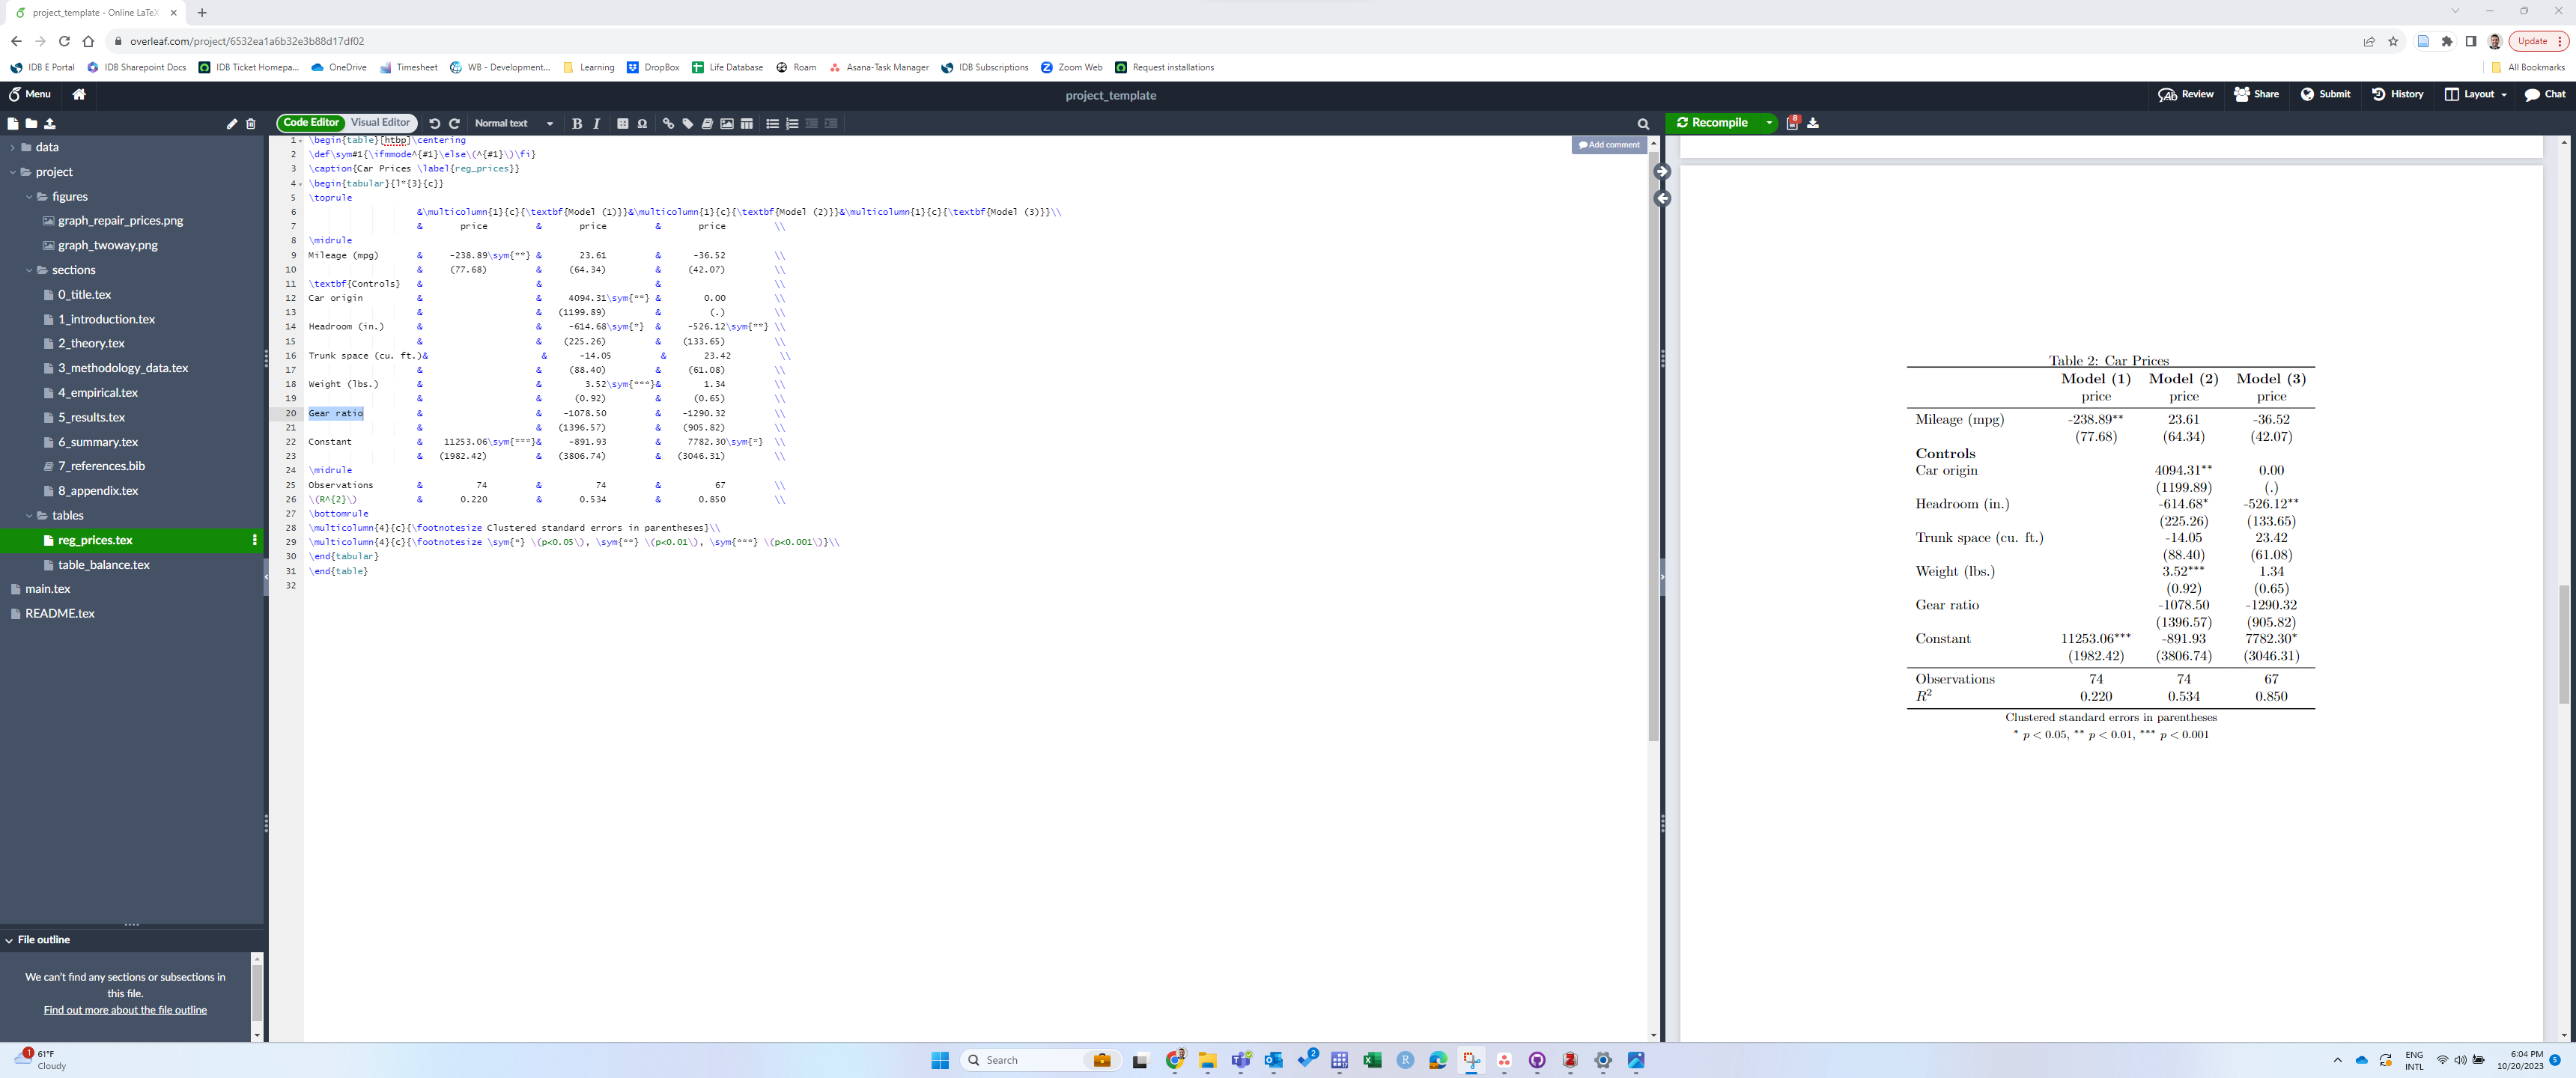
\includegraphics[width=1\textwidth]{Instructions/project_template_screenshots/project_template_26.png} \\

\section{Pushing Overleaf edits}

This was technically already demonstrated in the beginning, but just to further reinforce the understanding of this process, I'll demonstrate what happens now once the project is up and running. At this point, you have your results, and you are now writing a draft of your paper and have now written a few lines to the introduction. I have replaced \textbf{"Introduction test"} with, \textbf{"This is a test to demonstrate pushing changes made in Overleaf into my local storage"}. \\

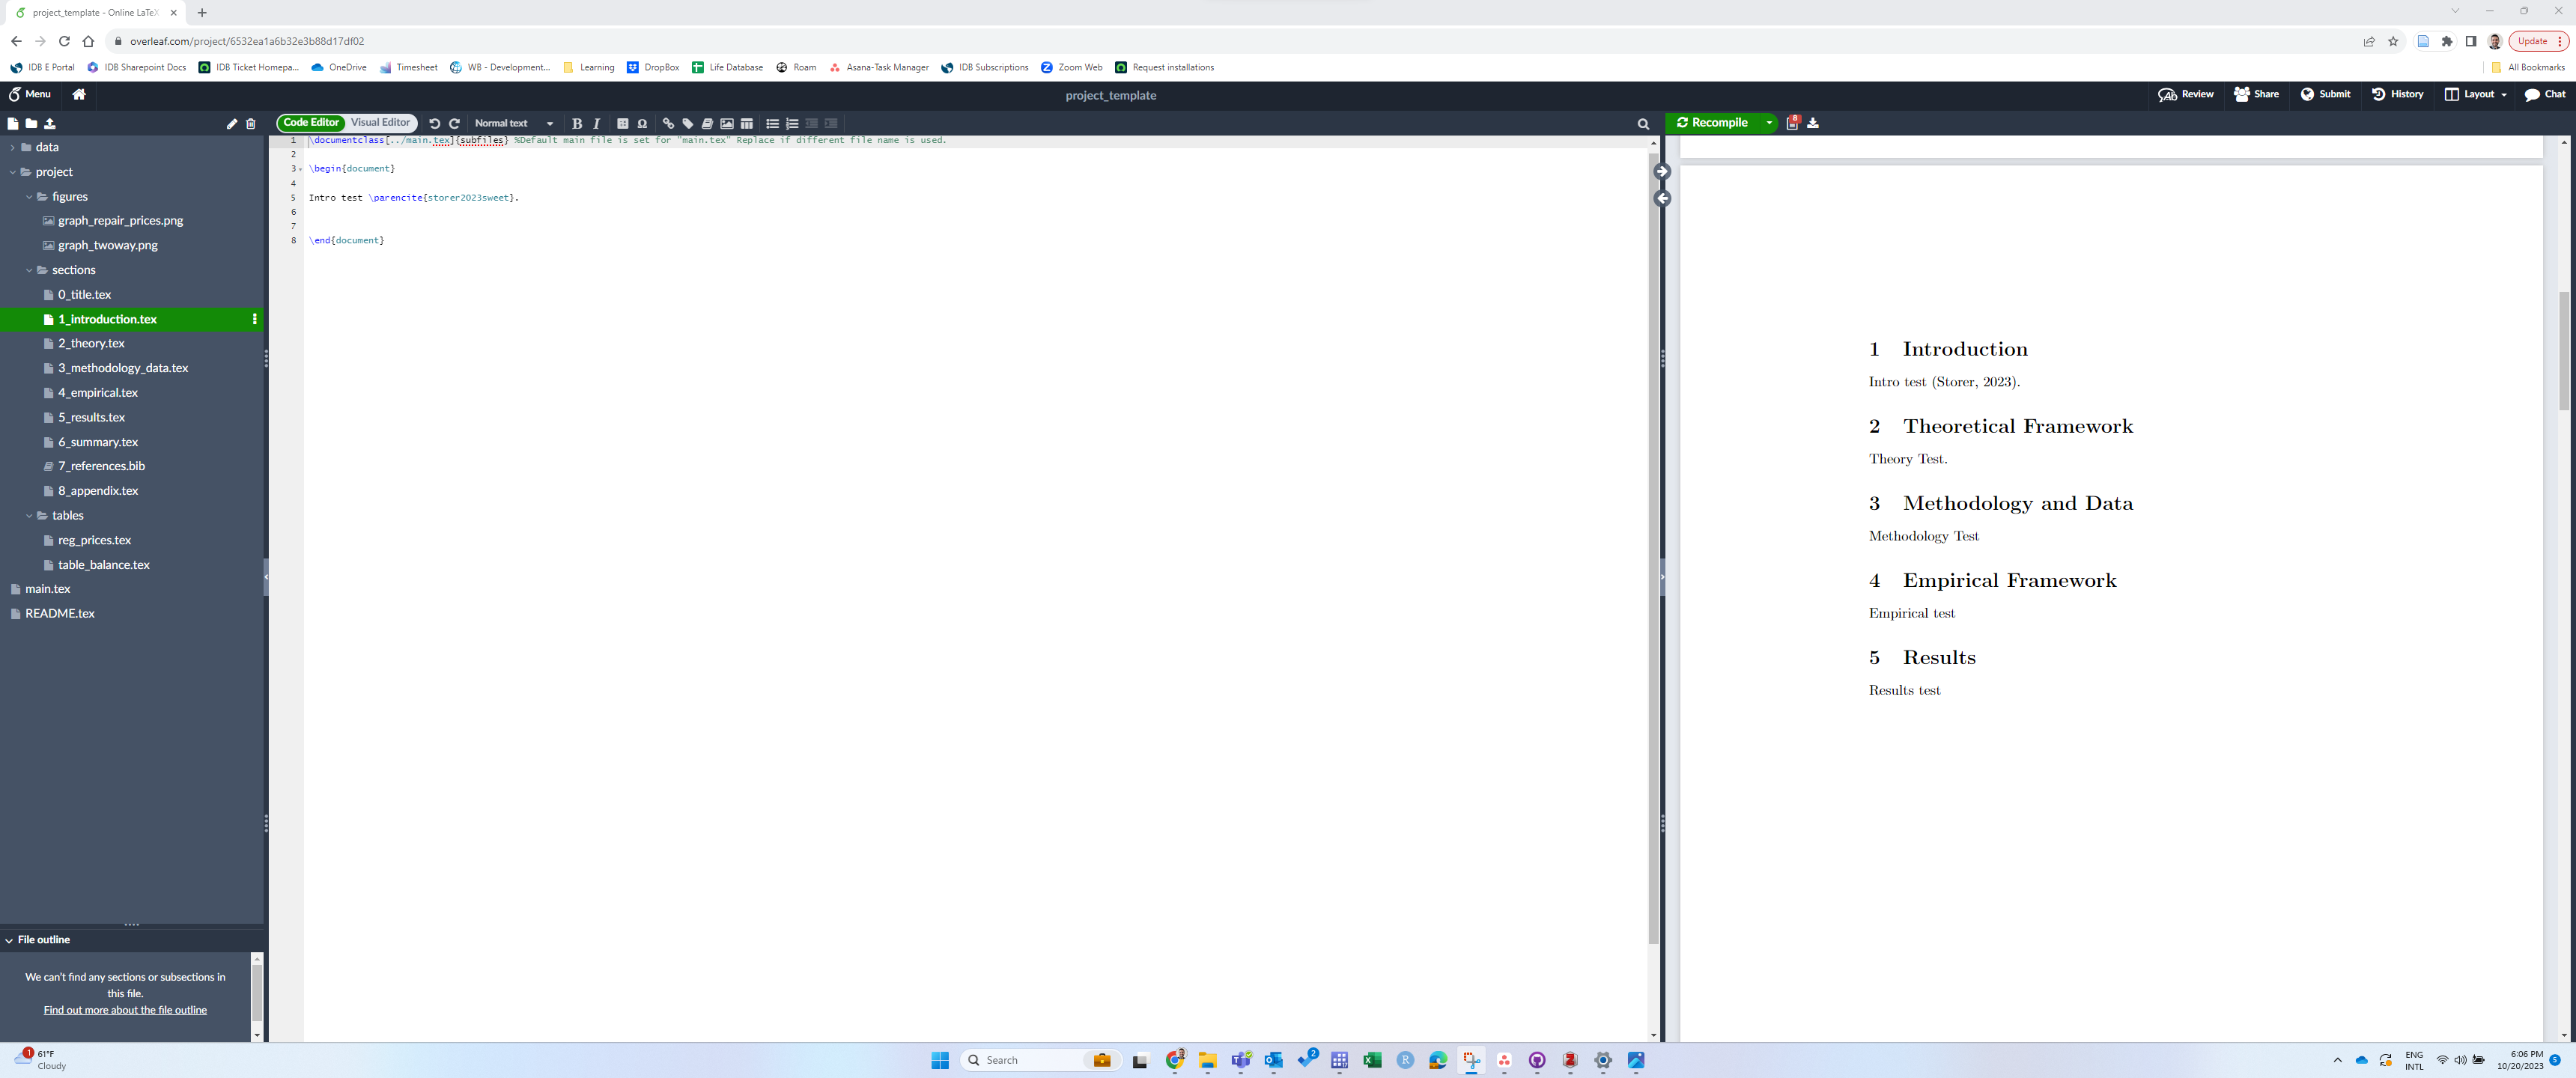
\includegraphics[width=1\textwidth]{Instructions/project_template_screenshots/project_template_27.png} \\

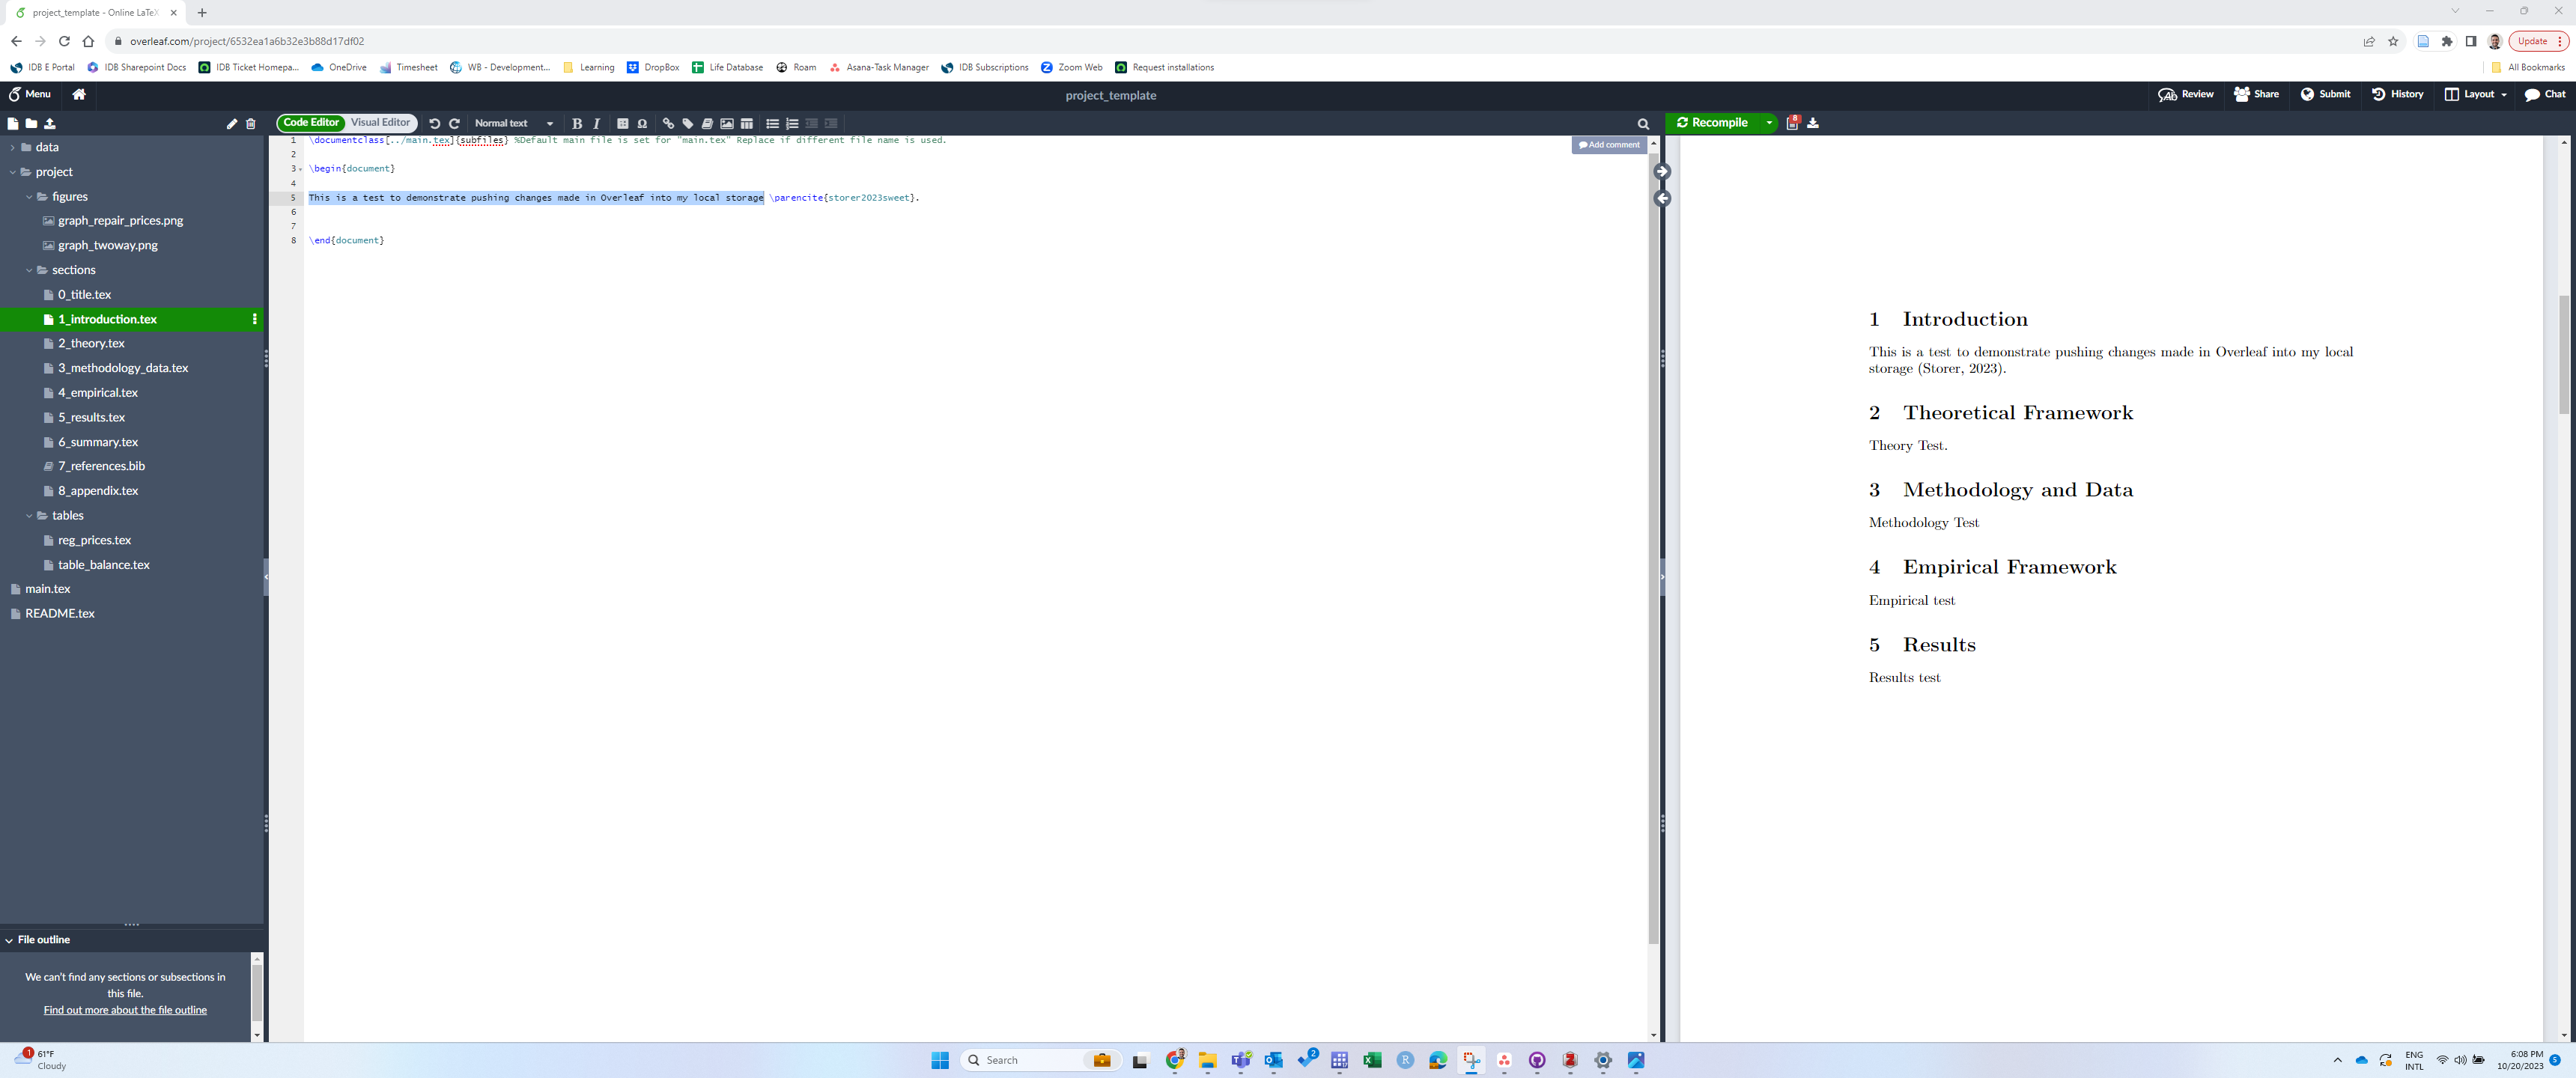
\includegraphics[width=1\textwidth]{Instructions/project_template_screenshots/project_template_28.png} \\

Select the GitHub menu option and now click on the \textbf{Push Overleaf changes to GitHub} button. \\

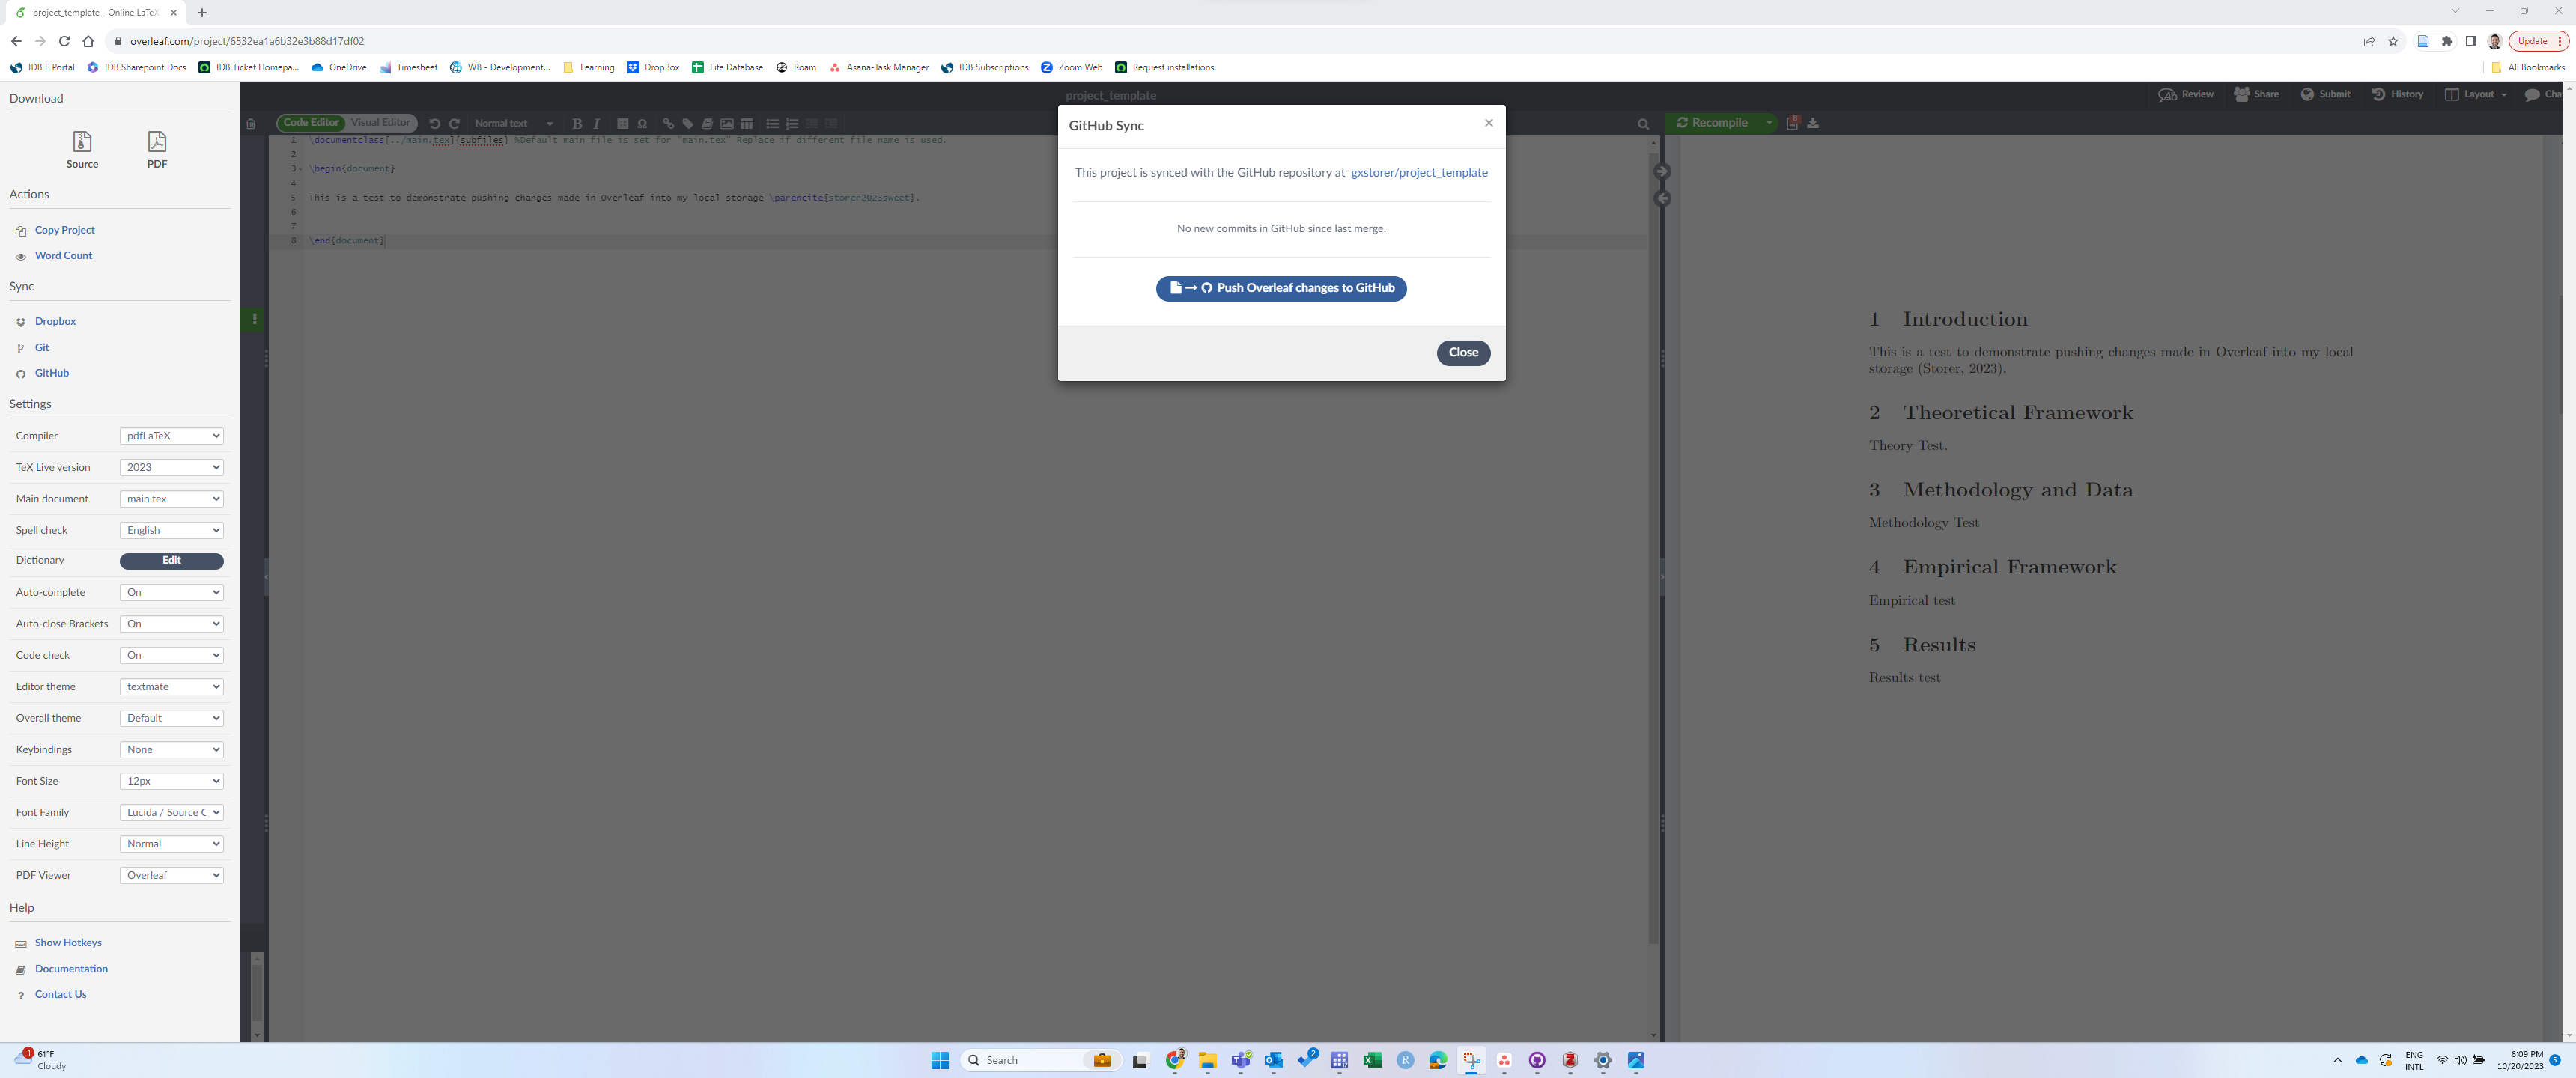
\includegraphics[width=1\textwidth]{Instructions/project_template_screenshots/project_template_29.png} \\

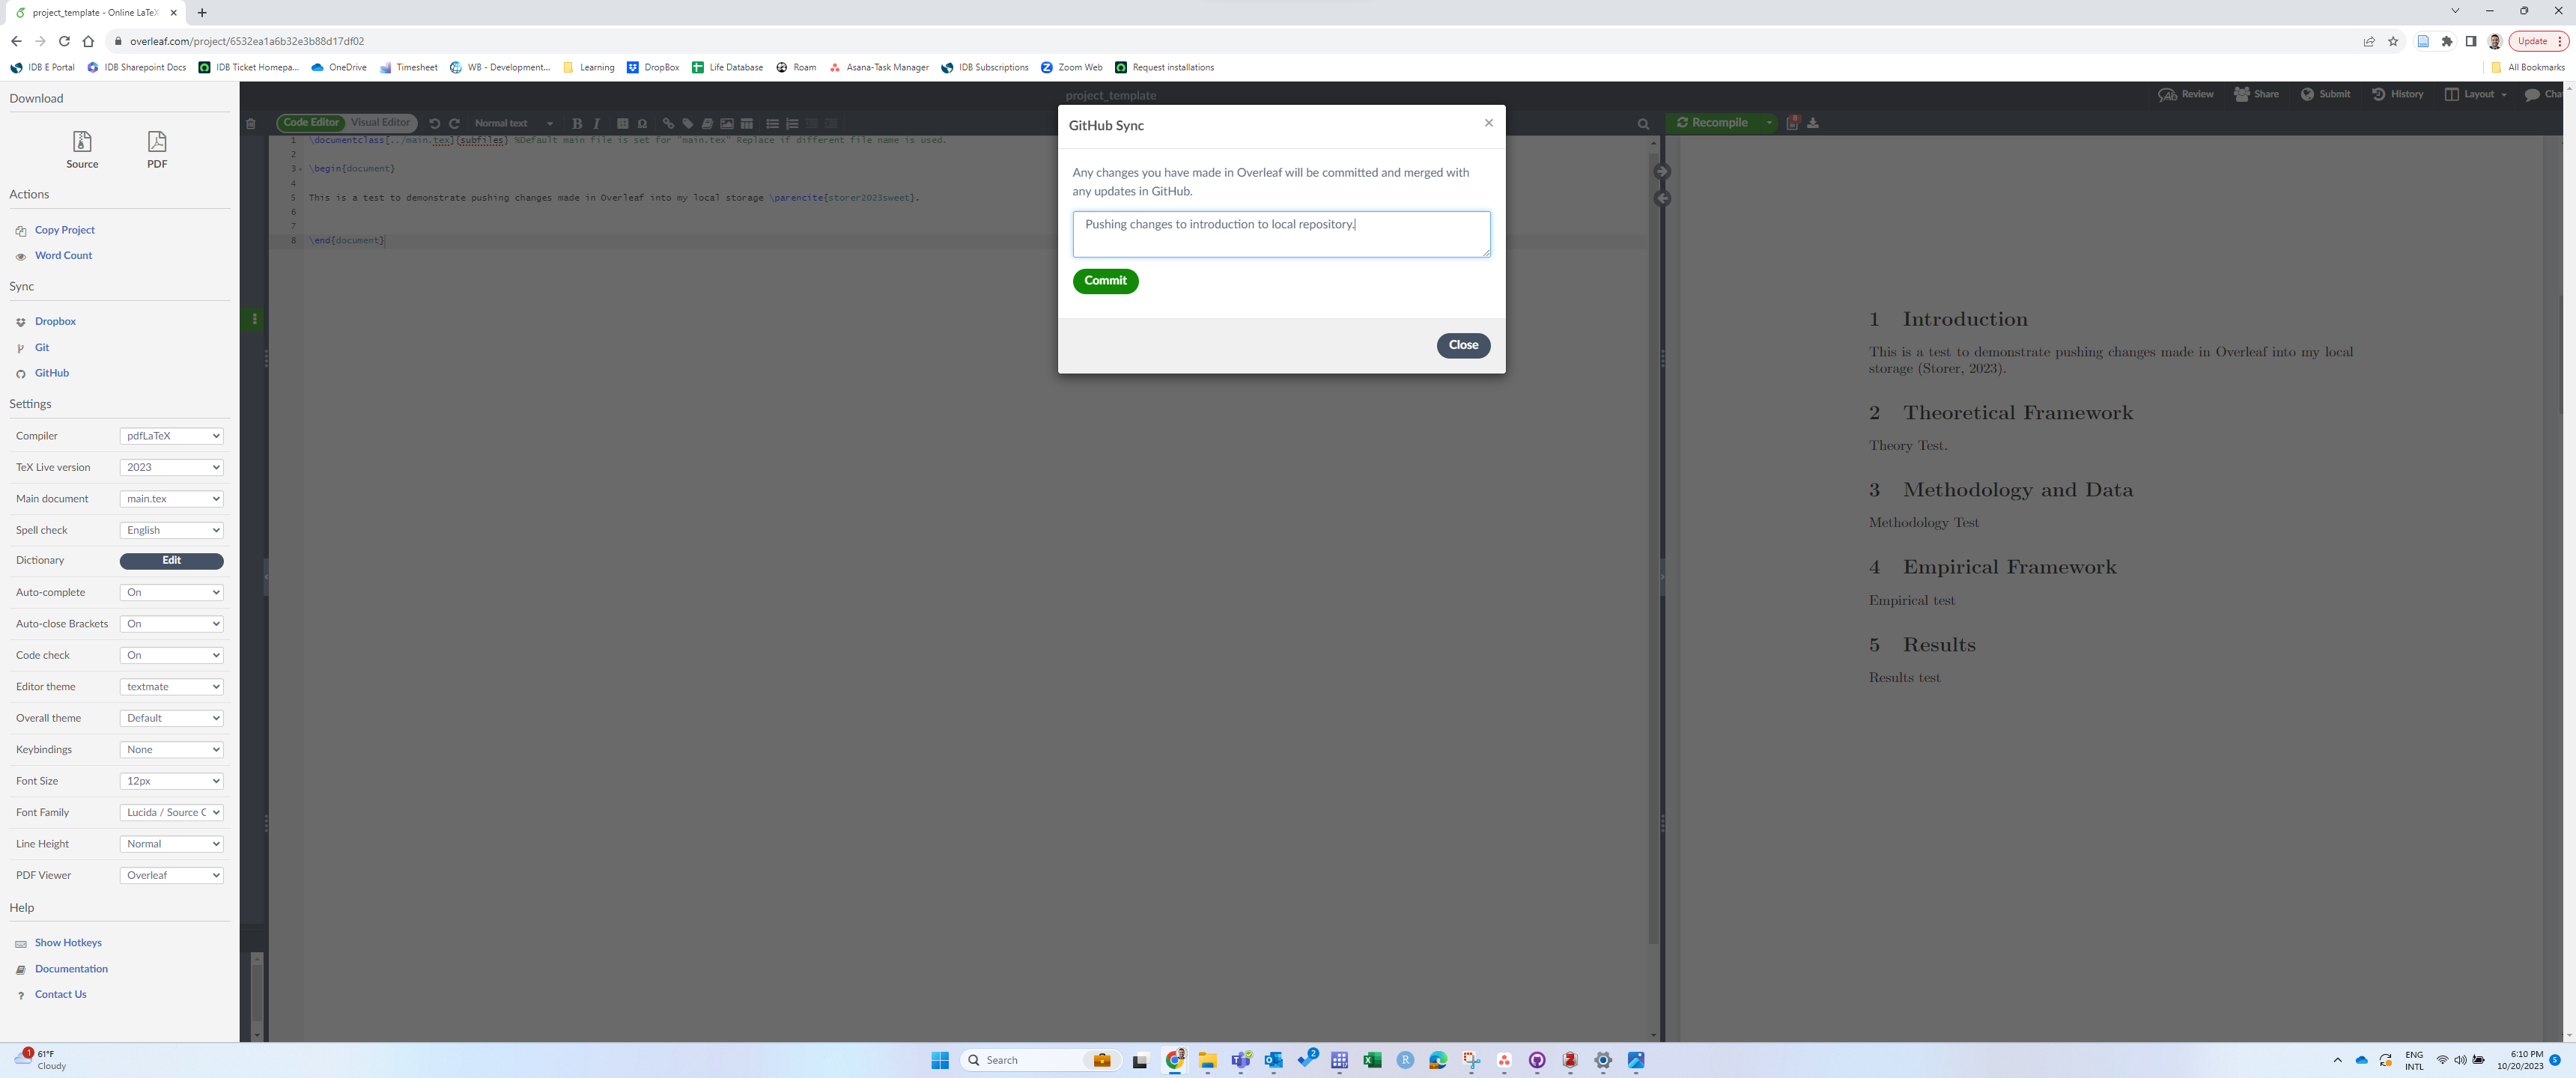
\includegraphics[width=1\textwidth]{Instructions/project_template_screenshots/project_template_30.png} \\

You can now see the changes made to the .tex file in your local repository once you pull changes in GitHub Desktop. \\

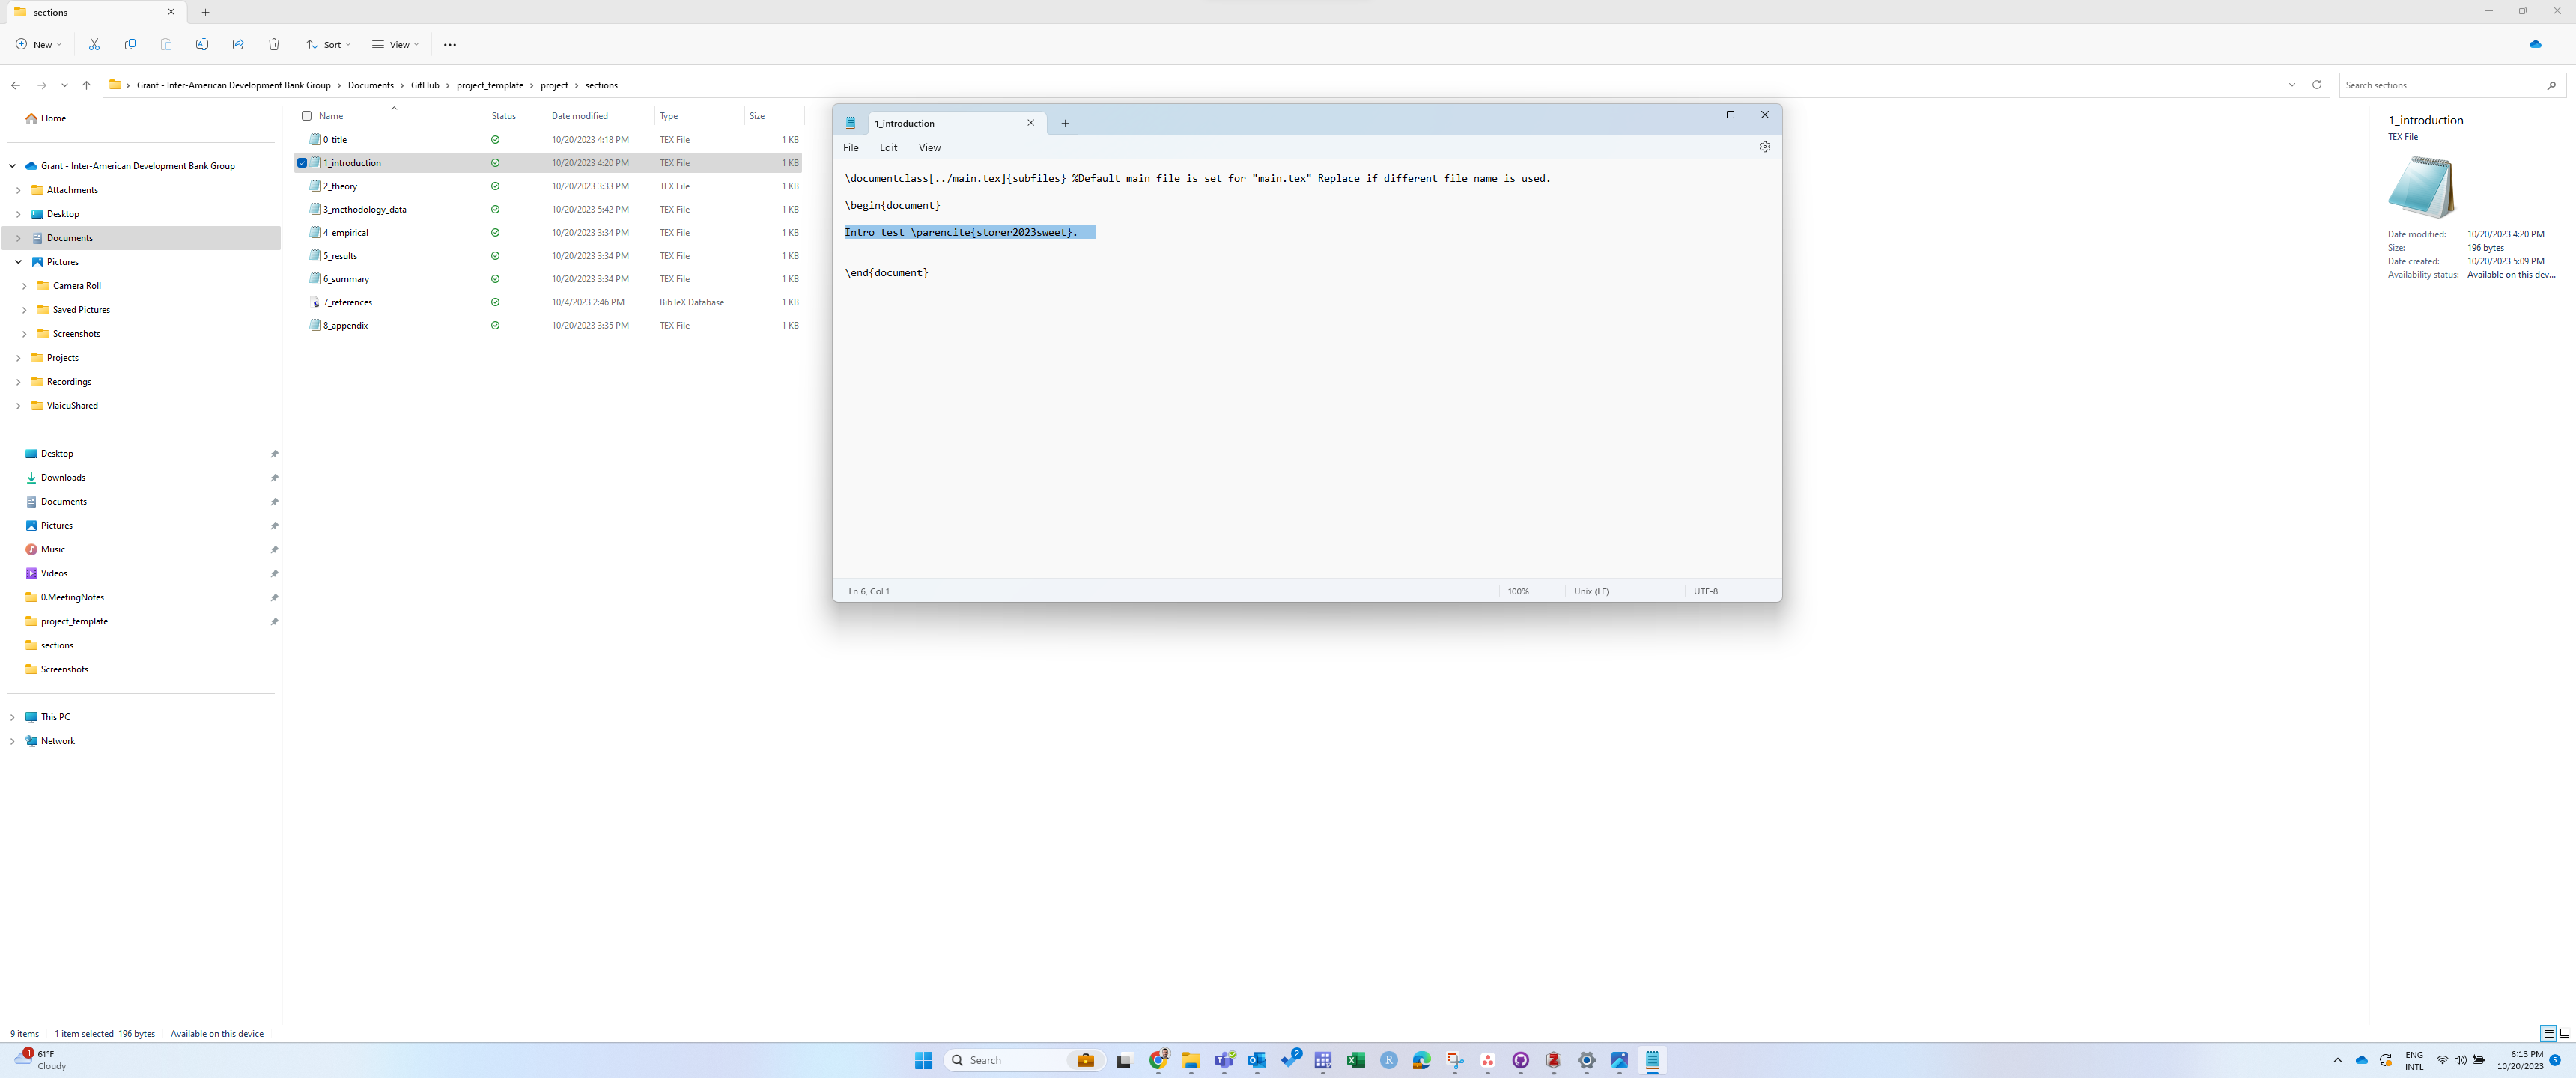
\includegraphics[width=1\textwidth]{Instructions/project_template_screenshots/project_template_31.png} \\

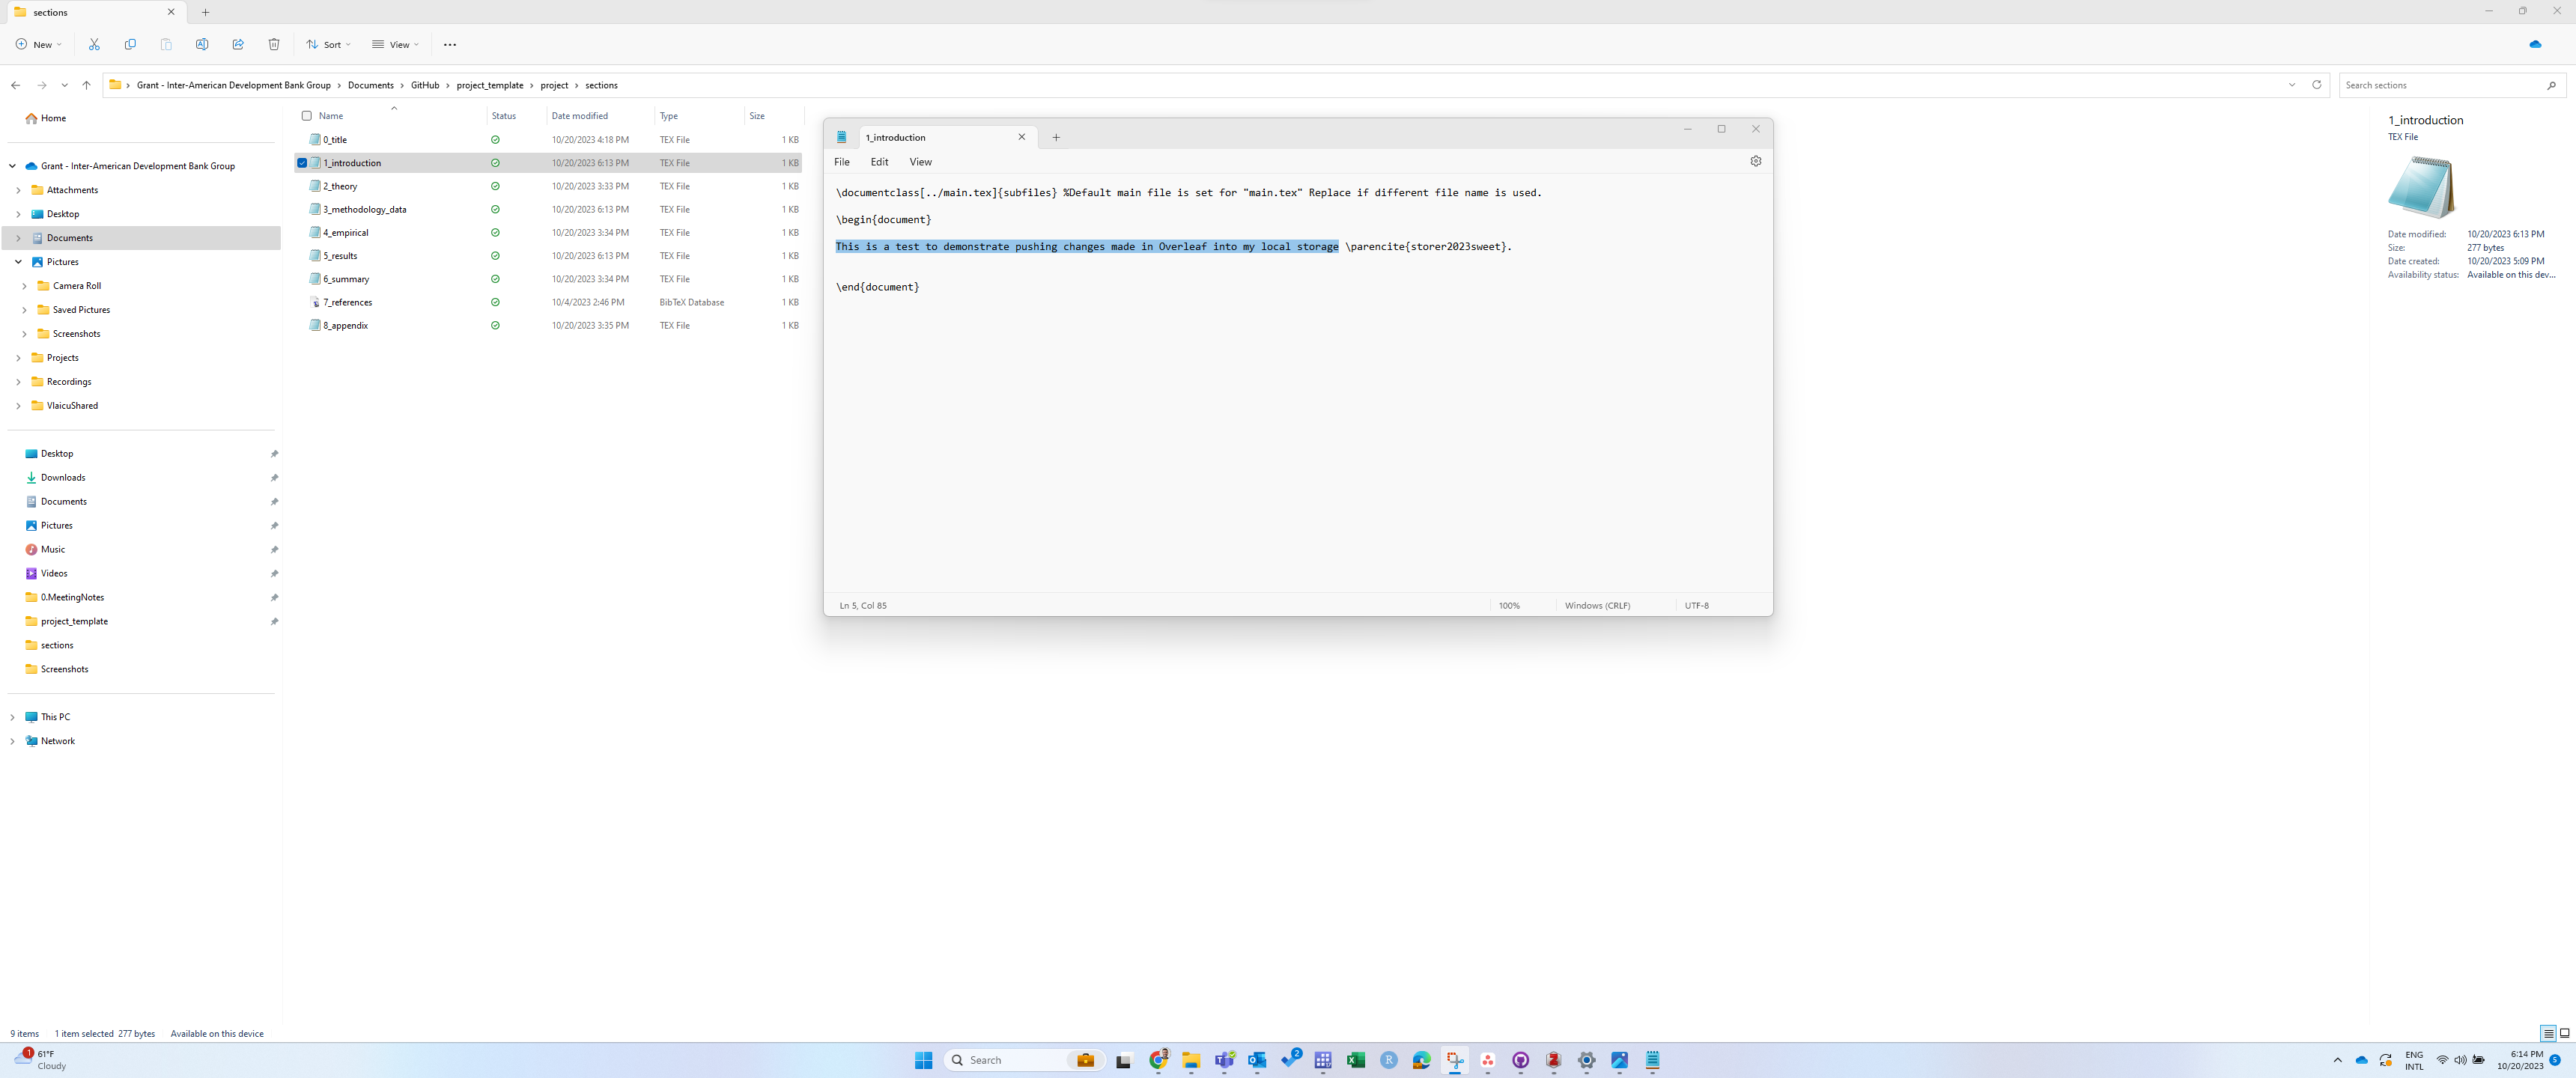
\includegraphics[width=1\textwidth]{Instructions/project_template_screenshots/project_template_33.png} \\

\section{Zotero Bibliography}

The last piece of automation is with the bibliography. Bibliographies can be quite tedious to manage, but thankfully Zotero make the process so much easier. Zotero is an web-based citation repository, where you can add extensions to your web browser that will not only download articles that you will use as references for your research, but also collect all the citation material needed as well. The following image is what my current library of saved articles looks like, where the left pane allows for file organization of saved articles, the middle pane displays the articles within the selected folder, and the right pane is the citation info of a selected article. \\

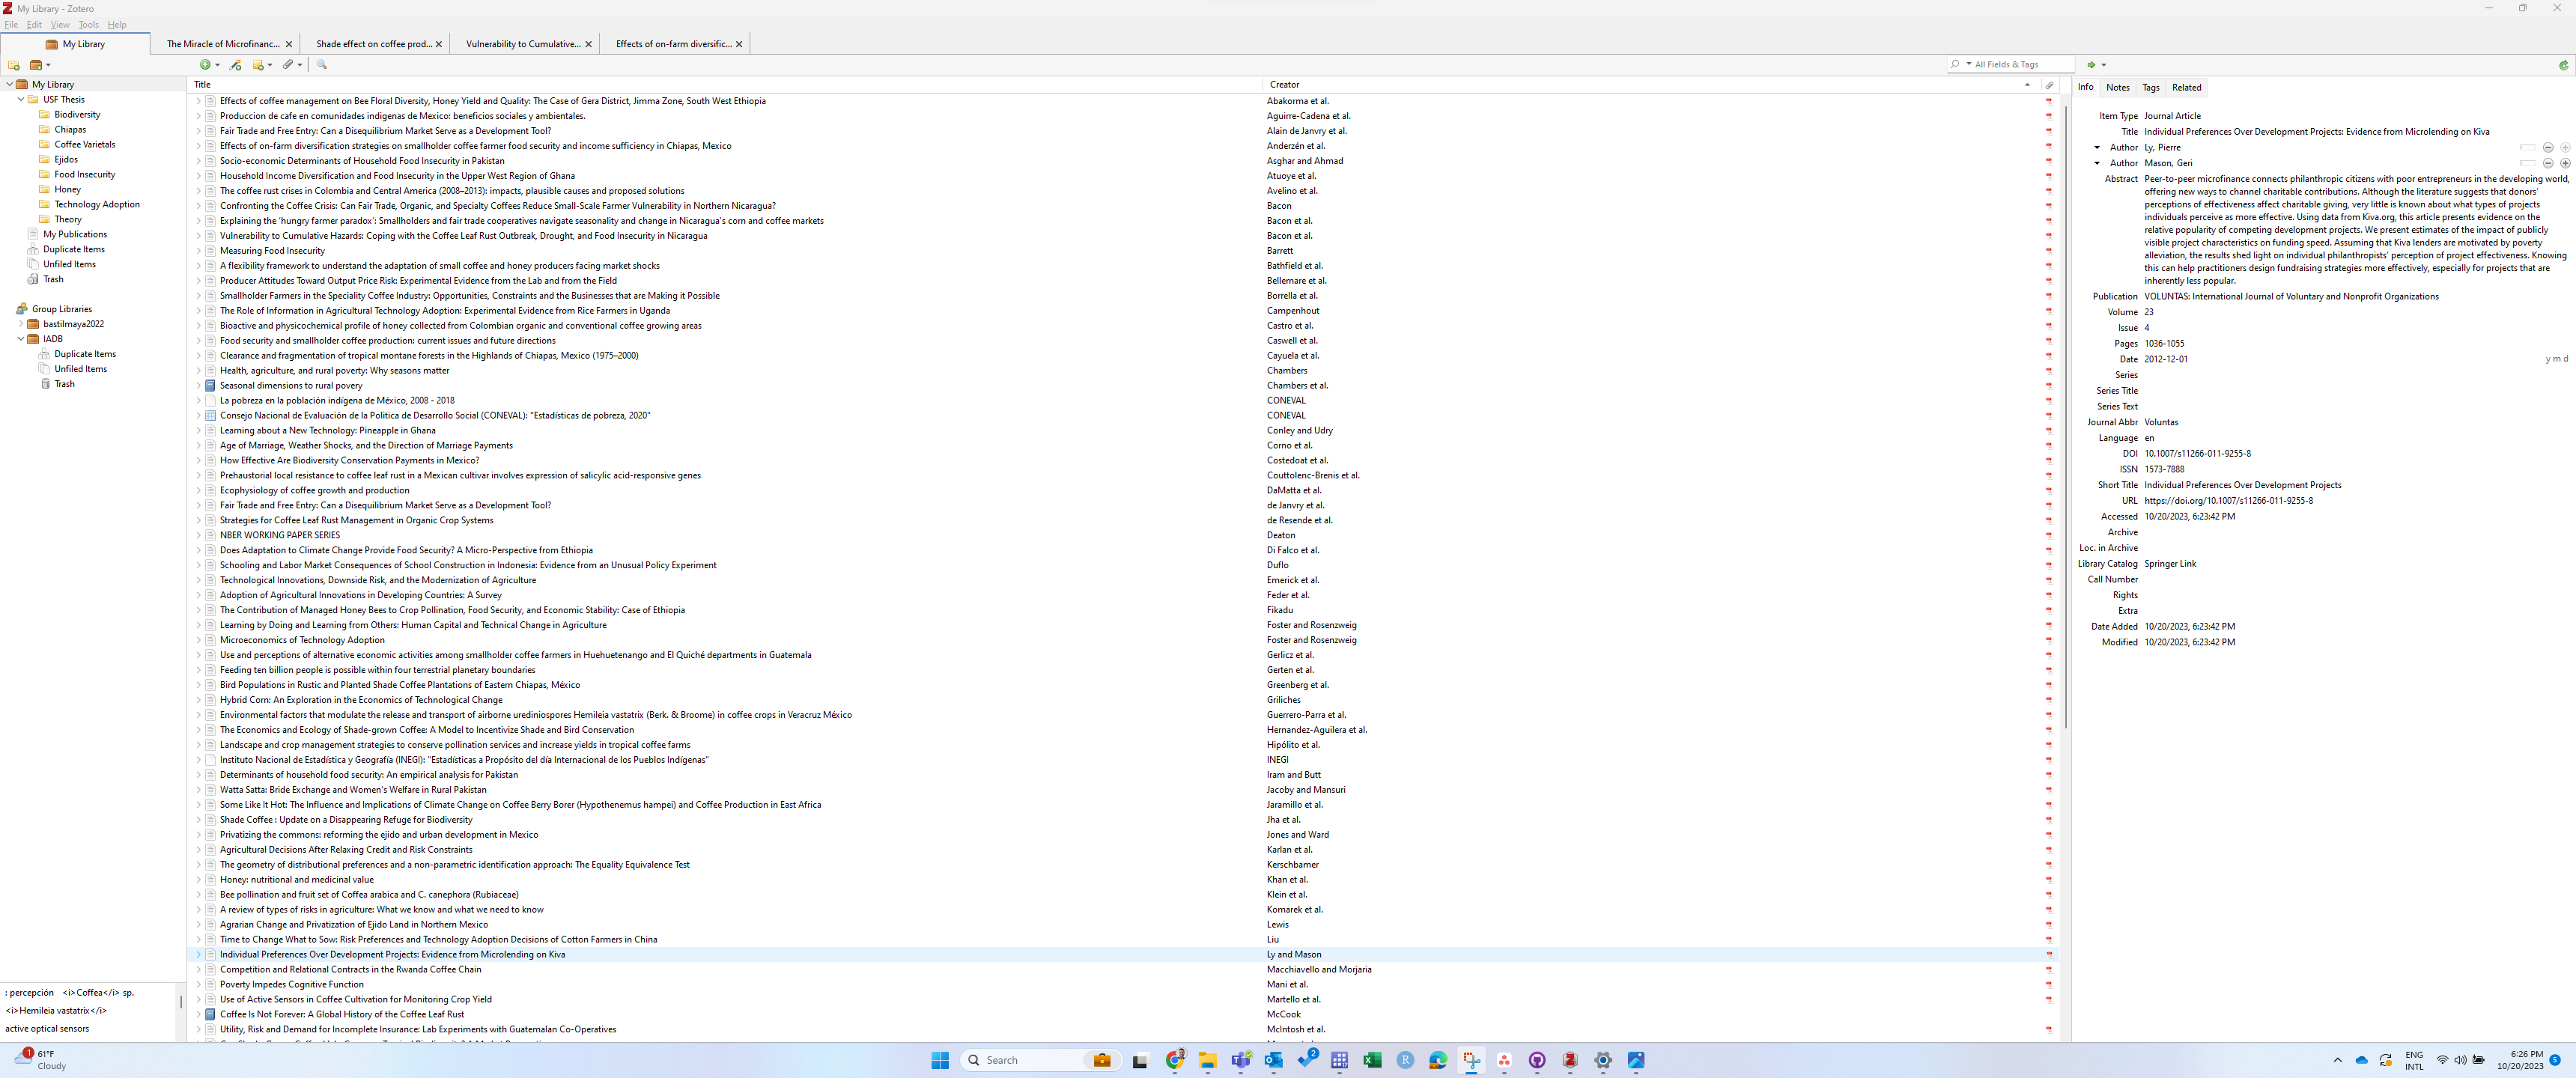
\includegraphics[width=1\textwidth]{Instructions/project_template_screenshots/project_template_35.png} \\

Zotero works with Overleaf, but operates in a slightly different way than how GitHub does for synchronization. To set up the connection, instead of going to the menu tab, you need to go to the \textbf{upload} tab that is below the menu tab. Once selected, you'll see there is an option labeled \textbf{"From Zotero"}, and asks from which library do you want to source from, along with the name of the reference file that you want it to be saved as in your project. The final option regarding format, use the updated version of BibTeX called \textbf{BibLaTeX}. \\

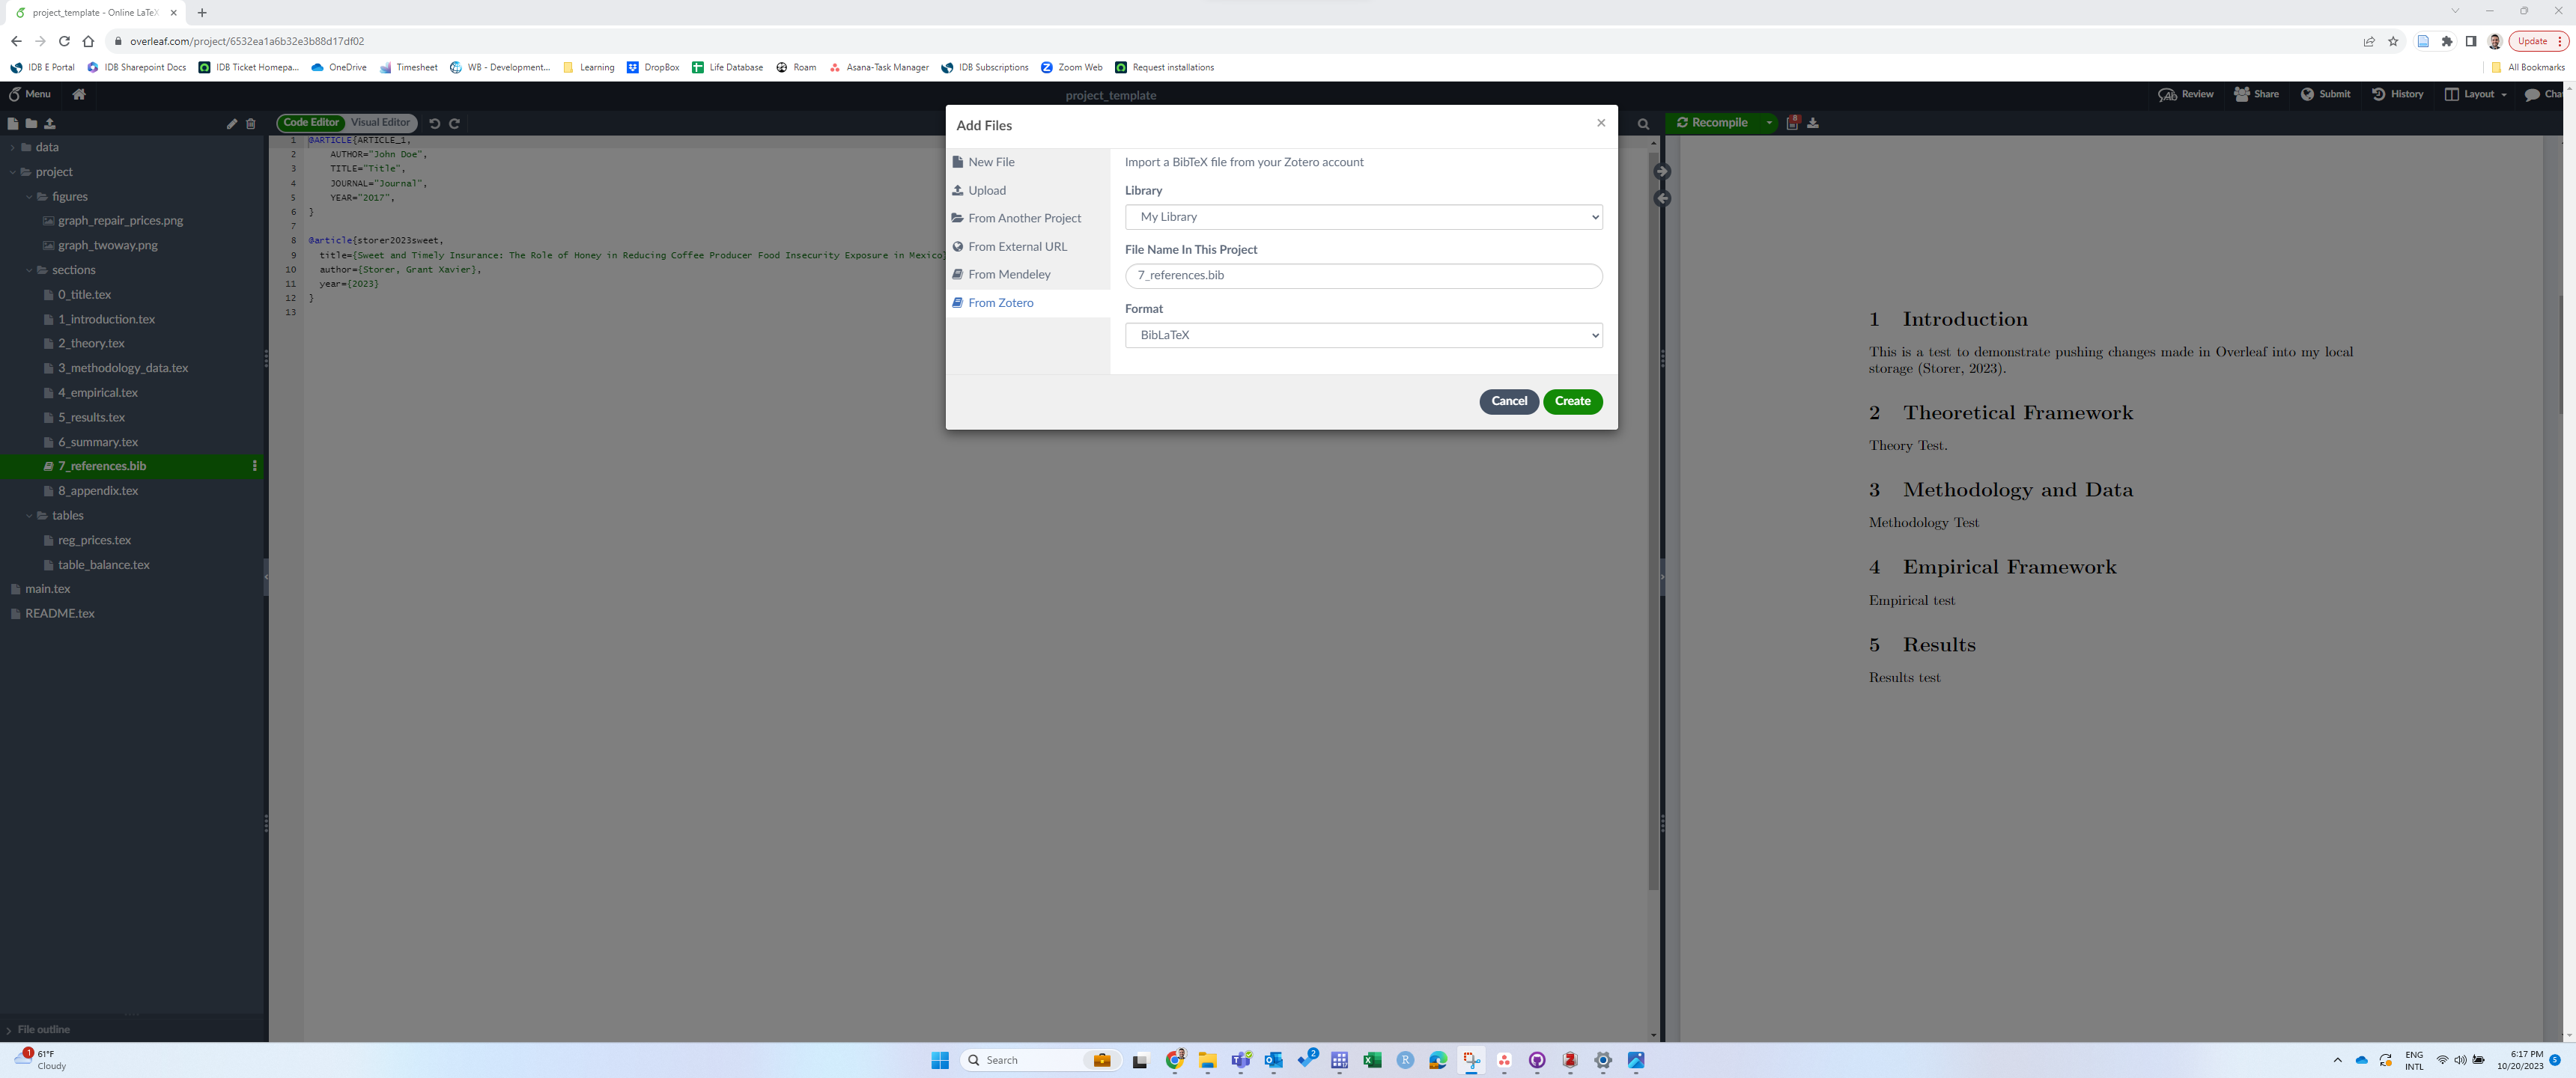
\includegraphics[width=1\textwidth]{Instructions/project_template_screenshots/project_template_34.png} \\

Once set up, you'll see a new file included in your project, but will have the .bib extension. You will now be able to cite anything you've saved in your Zotero in your paper, and your References section will only include those that have been actively used within your paper, no matter how many citations you have saved in your .bib file. 

If you ever add more citations to your Zotero, just click on the .bib file, and at the top there is a \textbf{refresh} button. Once selected, it will pull any new citations into your project that you'll be able to call up with the \textbf{cite} command. \\

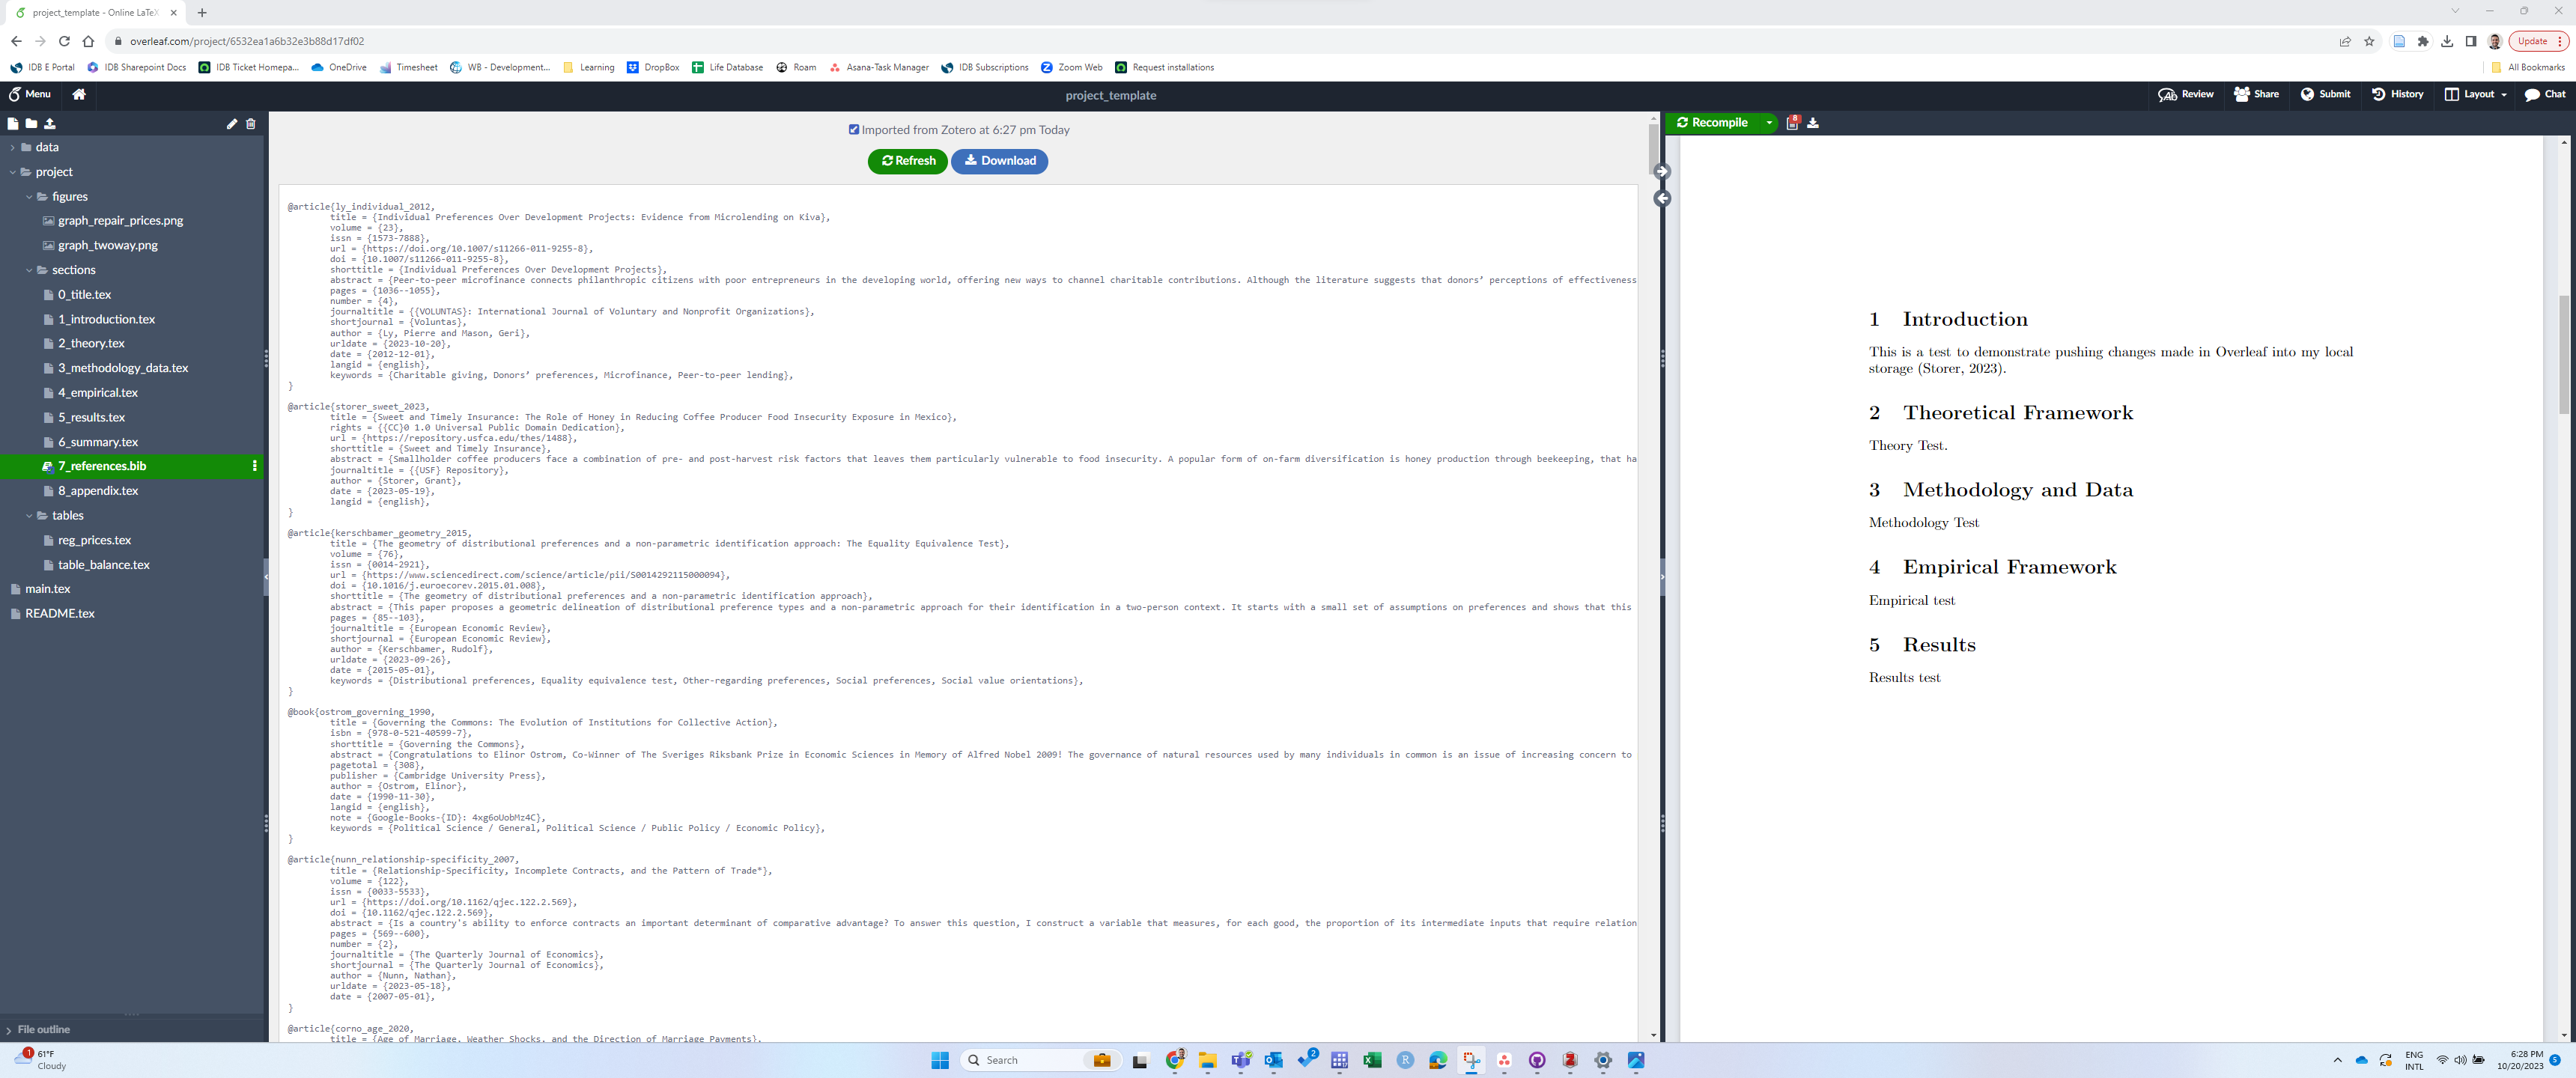
\includegraphics[width=1\textwidth]{Instructions/project_template_screenshots/project_template_36.png} \\

\section{Conclusion}

This is still a work-in-progress concept, and so I will be making changes in the future that will hopefully make this more accessible. If there are any elements that you're having difficulty understanding or replicating, that is a valuable indicator of the limits of what I've demonstrated, and would really appreciate you letting me know about that so I can make the necessary adjustments to make it better for other future users.  

I hope this can be useful for you, either by applying this format to your own projects, or by demonstrating alternative methods of operation that gives you the idea to modify your current method. Either way, that's a win for me. 

\end{document}